\documentclass[10pt]{article}
\usepackage[T1]{fontenc}
\usepackage{amsmath,amssymb,amsthm}
\usepackage[shortlabels]{enumitem}
\usepackage[english]{babel}
\usepackage[utf8]{inputenc}
\usepackage{fancyhdr}
\usepackage{bold-extra}
\usepackage{color}   
\usepackage{tocloft}
\usepackage{graphicx}
\usepackage{lipsum}
\usepackage{wrapfig}
\usepackage{cutwin}
\usepackage{hyperref}
\usepackage{lastpage}
\usepackage{multicol}
\usepackage{tikz}
 \usepackage{float}
\usetikzlibrary{patterns}

% some useful math commands
\newcommand{\eps}{\varepsilon}
\newcommand{\R}{\mathbb{R}}
\newcommand{\C}{\mathbb{C}}
\newcommand{\N}{\mathbb{N}}
\newcommand{\Z}{\mathbb{Z}}
\newcommand{\Q}{\mathbb{Q}}
\newcommand{\K}{\mathbb{K}}
\newcommand{\F}{\mathbb{F}}

\newcommand{\dd}{\,{\rm d}}

\DeclareMathOperator{\Ber}{Bernoulli}
\DeclareMathOperator{\Bin}{Bin}
\DeclareMathOperator{\Multi}{Multi}
\DeclareMathOperator{\Poi}{Poi}
\DeclareMathOperator{\UNIF}{UNIF}
\DeclareMathOperator{\EXP}{EXP}
\DeclareMathOperator{\Nor}{N}
\DeclareMathOperator{\GAM}{GAM}
\DeclareMathOperator{\BETA}{BETA}
\DeclareMathOperator{\MLE}{MLE}
\DeclareMathOperator{\Var}{Var}
\DeclareMathOperator{\Cov}{Cov}
\DeclareMathOperator{\argmax}{argmax}
\DeclareMathOperator{\Bias}{Bias}
\DeclareMathOperator{\Eff}{Eff}
\DeclareMathOperator{\MSE}{MSE}

% title formatting
\newcommand{\newtitle}[4]{
  \begin{center}
	\huge{\textbf{\textsc{#1 Course Notes}}}
    
	\large{\sc #2}
    
	{\sc #3 \textbullet\, #4 \textbullet\, University of Waterloo}
	\normalsize\vspace{1cm}\hrule
  \end{center}
}

% for theorems
\newtheoremstyle{newstyle}      
{} %Aboveskip 
{-0.25pt} %Below skip
{\mdseries} %Body font e.g.\mdseries,\bfseries,\scshape,\itshape
{} %Indent
{\scshape} %Head font e.g.\bfseries,\scshape,\itshape
{.} %Punctuation afer theorem header
{ } %Space after theorem header
{} %Heading

\theoremstyle{newstyle}

\newtheorem*{prop*}{Proposition}
\newtheorem*{cor*}{Corollary}
\newtheorem*{exercise*}{Exercise}
\newtheorem*{lemma*}{Lemma}
\newtheorem*{remark*}{Remark}
\newtheorem*{exmp*}{Example}
\newtheorem*{defn*}{Definition}
\newtheorem*{thm*}{Theorem}
\newtheorem*{notation*}{Notation}
\newtheorem{thm}{Theorem}[section]
\newtheorem{fact}[thm]{Fact}
\newtheorem{cor}[thm]{Corollary}
\newtheorem{lemma}[thm]{Lemma}
\newtheorem{remark}[thm]{Remark}
\newtheorem{prop}[thm]{Proposition}
\newtheorem{defn}[thm]{Definition}
\newtheorem{claim}[thm]{Claim}
\newtheorem{axiom}[thm]{Axiom}
\newtheorem{notation}[thm]{Notation}
\newtheorem{exercise}[thm]{Exercise}
\newtheorem{exmp}[thm]{Example}

% new proof environment
\makeatletter
\newenvironment{pf}[1][\proofname]{\par
  \pushQED{\qed}%
  \normalfont \topsep0\p@\relax
  \trivlist
  \item[\hskip\labelsep\scshape
  #1\@addpunct{.}]\ignorespaces
}{%
  \popQED\endtrivlist\@endpefalse
}
\makeatother

% 1-inch margins
\topmargin 0pt
\advance \topmargin by -\headheight
\advance \topmargin by -\headsep
\textheight 8.9in
\oddsidemargin 0pt
\evensidemargin \oddsidemargin
\marginparwidth 0.5in
\textwidth 6.5in

% \renewcommand{\headrulewidth}{0pt}
% \renewcommand{\footrulewidth}{0.4pt}

\parindent 0in
\parskip 1.5ex

\setlist[itemize]{topsep=0pt}
\setlist[enumerate]{topsep=0pt}

% hyperlinks
\hypersetup{
  colorlinks=true, 
  linktoc=all,     % table of contents is clickable  
  allcolors=black  % all hyperlink colours
}

% table of contents
\addto\captionsenglish{
  \renewcommand{\contentsname}%
    {Table of Contents}%
}
\renewcommand{\cftsecfont}{\normalfont}
\renewcommand{\cftsecpagefont}{\normalfont}
\cftsetindents{section}{0em}{2em}

\fancypagestyle{plain}{%
\fancyhf{} % clear all header and footer fields
\lhead{STAT 241: Winter 2021}
\fancyhead[R]{Table of Contents}
%\headrule
\fancyfoot[R]{{\small Page \thepage\ of \pageref*{LastPage}}}
}

% headers and footers
\pagestyle{fancy}
\renewcommand{\sectionmark}[1]{\markboth{#1}{#1}}
\lhead{STAT 241: Winter 2021}
\cfoot{}
\setlength\headheight{14pt}

% \setcounter{section}{-1}

\begin{document}

\pagestyle{fancy}
\newtitle{STAT 241}{Statistics (Advanced Level)}{Yingli Qin}{Winter 2021}
\rhead{Table of Contents}
\rfoot{{\small Page \thepage\ of \pageref*{LastPage}}}

\tableofcontents
\vspace{1cm}\hrule
\fancyhead[R]{Week \thesection: \leftmark}
\newpage 
% \thispagestyle{empty}

\section{Review}

\subsection{Cumulative distribution function}

\begin{defn} 
The {\bf cumulative distribution function (CDF)} of a random variable $X$ is defined by 
\[ F(x) = P(X \leq x), \quad x \in \R. \]
\end{defn}
{\bf Properties of the CDF.} Let $F$ be the CDF of a random variable $X$. Then:
\begin{enumerate}[(1)]
    \item $F$ is non-decreasing; that is, $F(x_1) \leq F(x_2)$ for all $x_1 < x_2$. 
    \item $\lim_{x\to-\infty} F(x) = 0$ and $\lim_{x\to\infty} F(x) = 1$.
    \item $F$ is right-continuous; that is, $\lim_{x\to a^+} F(x) = F(a)$ for $a \in \R$.
    \item For $a < b \in \R$, we have $P(a < X \leq b) = P(X \leq b) - P(X \leq a) = F(b) - F(a)$.
    \item Given $b \in \R$, we have $P(X = b) = P(X \leq b) - P(X < b) = F(b) - \lim_{a\to b^-} F(a)$.
\end{enumerate}

Note that the definition and the above properties hold for any random variable $X$ regardless of 
whether $X$ is discrete or continuous.

\subsection{Discrete random variables and their probability functions}

\begin{defn}
If $X$ takes finitely or countably many values, then $X$ is said to be a {\bf discrete random variable}.
In this case, the CDF $F$ of $X$ is a right-continuous step function.
\end{defn}

\begin{defn}
If $X$ is a discrete random variable, then the {\bf probability function (PF)} of $X$ is given by 
\[ f(x) = P(X = x), \quad x \in A. \] 
The set $A = \{x \in \R : f(x) > 0\}$ is called the {\bf support set} of $X$.
\end{defn}
{\bf Properties of the PF.} Let $f$ be the PF of a discrete random variable $X$. Then: 
\begin{enumerate}[(1)]
    \item For all $x \in \R$, we have $f(x) \geq 0$, and the inequality is strict if $x \in A$. 
    \item $\sum_{x \in A} f(x) = 1$.
\end{enumerate}

\begin{exmp}
Suppose that $X$ only takes the values $0$ and $1$, with $P(X = 0) = P(X = 1) = 1/2$. Then the 
CDF of $X$ is given by 
\[ F(x) = P(X \leq x) = \begin{cases} 0 & x < 0 \\ 1/2 & 0 \leq x < 1 \\ 1 & x \geq 1. \end{cases} \]
As seen in the graph below, $F$ is indeed a right-continuous step function.
\begin{center}
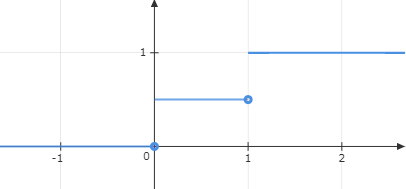
\includegraphics[width=0.5\textwidth]{example1.png}
\end{center}
\end{exmp}

\subsection{More examples of discrete random variables}

The discrete random variable $X$ in Example 1.4 can naturally be extended to other discrete random
variables that we are familiar with. 

{\bf Bernoulli.}
Suppose that $X \sim \Ber(\theta)$ for some $0 < \theta < 1$. Then 
$P(X = 1) = \theta$ and $P(X = 0) = 1-\theta$, where a $1$ is a success, and a $0$ is a failure. 

{\bf Binomial.}
Let $0 < \theta < 1$. Suppose that $X_i \sim \Ber(\theta)$ for all $1 \leq i \leq n$, 
and that the $X_i$'s are independent. 
Then, we may define the discrete random variable
\[ X = \sum_{i=1}^n X_i. \]
Essentially, this is the number of successes in a sequence of independent and identically distributed
(i.i.d.) $\Ber(\theta)$ random variables. This is the binomial distribution; 
that is, $X \sim \Bin(n, \theta)$. The support set of $X$ is $A = \{0, 1, \dots, n\}$, and 
we have 
\[ P(X = x) = \binom{n}{x} \theta^x (1-\theta)^{n-x}. \]

{\bf Multinomial.} Suppose that $(X_1, X_2, \dots, X_k) \sim \Multi(n, \theta_1, \theta_2, \dots, 
\theta_k)$. 
For each trial, there are $k+1$ possible outcomes, with corresponding probabilities 
$(\theta_1, \theta_2, \dots, \theta_k, 1 - \sum_{i=1}^k \theta_i)$. For convenience, it is useful to 
denote $\theta_{k+1} := 1 - \sum_{i=1}^k \theta_i$. Then, for each $1 \leq i \leq k$, we let 
$X_i$ be the number of times outcome $i$ occurs in $n$ trials. 
Writing $x_{k+1} := n - \sum_{i=1}^k x_i$, the probability function of $X$ is given by 
\[ P(X_1 = x_1, \dots, X_k = x_k) = \frac{n!}{x_1!x_2! \cdots x_k! x_{k+1}!} 
\theta_1^{x_1} \theta_2^{x_2} \cdots \theta_k^{x_k} \theta_{k+1}^{x_{k+1}} \]

{\bf Poisson.} Suppose that $X \sim \Poi(\mu)$ for some $\mu > 0$. Often, $X$ denotes the 
number of events during a time period, and $\mu$ is the occurrence rate (that is, 
$\mu = E(x)$). The probability function of $X$ is given by 
\[ f(x) = P(X = x) = \frac{\mu^x e^{-\mu}}{x!}, \quad x \in \Z_{\geq 0}. \]
Notice that we have 
\[ \sum_{x=0}^\infty f(x) = \sum_{x=0}^\infty \frac{\mu^x e^{-\mu}}{x!} = 
e^{-\mu} \sum_{x=0}^\infty \frac{\mu^x}{x!} = e^{-\mu} e^\mu = 1. \]

\subsection{Continuous random variables and their probability density functions}

\begin{defn}
Suppose $X$ is a random variable with CDF $F$. If $F$ is continuous at each $x \in \R$ and 
$F$ is differentiable except possibly at countably many points, then $X$ is said to be a 
{\bf continuous random variable}.
\end{defn}

\begin{defn}
If $X$ is a continuous random variable with CDF $F$, then the {\bf probability 
density function (PDF)} of $X$ is given by 
\[ f(x) = \begin{cases} F'(x) & \text{if $F$ is differentiable at $x$} \\ 0 & \text{otherwise.} \end{cases}
\]
The set $A = \{x \in \R : f(x) > 0\}$ is called the {\bf support set} of $X$.
\end{defn}

\newpage 
{\bf Properties of the PDF.} Suppose $f$ is the PDF of a continuous random variable $X$.
Then:\begin{enumerate}[(1)]
    \item For all $x \in \R$, we have $f(x) \geq 0$.
    \item $\int_{-\infty}^\infty f(x)\,{\rm d}x = \lim_{x\to\infty} F(x) - \lim_{x\to-\infty} F(x) 
    = 1 - 0 = 1.$
    \item For all $x \in \R$, we have $F(x) = \int_{-\infty}^x f(t)\,{\rm d}t$. \vspace{-1ex}
    \item $P(a < X \leq b) = P(X \leq b) - P(X \leq a) = F(b) - F(a) = \int_a^b f(x) \, {\rm d}x$.
    \item $P(X = b) = F(b) - \lim_{a\to b^-} F(a) = F(b) - F(b) = 0$ (since $F$ is continuous).
\end{enumerate}

\subsection{Examples of continuous random variables}

{\bf Uniform.} Suppose $X$ is a random variable with CDF 
\[ F(x) = \begin{cases} 0 & x \leq a \\ \frac{x-a}{b-a} & a < x < b \\ 1 & x \geq b, \end{cases} \]
where $a < b$. The graph of the CDF is below. 
\begin{center}
\tikzset{every picture/.style={line width=0.75pt}} %set default line width to 0.75pt        
\begin{tikzpicture}[x=0.75pt,y=0.75pt,yscale=-1,xscale=1]
%uncomment if require: \path (0,438); %set diagram left start at 0, and has height of 438
%Straight Lines [id:da8568107343979088] 
\draw    (60,160) -- (204.5,160) -- (270,160) ;
%Straight Lines [id:da8783789887412872] 
\draw    (130,60) -- (130,190) ;
%Straight Lines [id:da5801298716477992] 
\draw [color={rgb, 255:red, 74; green, 144; blue, 226 }  ,draw opacity=1 ]   (60,160) -- (160,160) ;
\draw [shift={(160,160)}, rotate = 0] [color={rgb, 255:red, 74; green, 144; blue, 226 }  ,draw opacity=1 ][fill={rgb, 255:red, 74; green, 144; blue, 226 }  ,fill opacity=1 ][line width=0.75]      (0, 0) circle [x radius= 3.35, y radius= 3.35]   ;
%Straight Lines [id:da391705509902899] 
\draw [color={rgb, 255:red, 74; green, 144; blue, 226 }  ,draw opacity=1 ]   (160,160) -- (210,100) ;
\draw [shift={(210,100)}, rotate = 309.81] [color={rgb, 255:red, 74; green, 144; blue, 226 }  ,draw opacity=1 ][fill={rgb, 255:red, 74; green, 144; blue, 226 }  ,fill opacity=1 ][line width=0.75]      (0, 0) circle [x radius= 3.35, y radius= 3.35]   ;
%Straight Lines [id:da36572029052125865] 
\draw [color={rgb, 255:red, 74; green, 144; blue, 226 }  ,draw opacity=1 ]   (210,100) -- (270,100) ;

% Text Node
\draw (157,168.4) node [anchor=north west][inner sep=0.75pt]    {$a$};
% Text Node
\draw (206.5,163.4) node [anchor=north west][inner sep=0.75pt]    {$b$};
% Text Node
\draw (118,40.4) node [anchor=north west][inner sep=0.75pt]    {$F(x)$};
% Text Node
\draw (272,156.4) node [anchor=north west][inner sep=0.75pt]    {$x$};
\end{tikzpicture}\end{center}
Notice that $F$ is continuous at every $x \in \R$ and differentiable except at the points 
$x = a$ and $x = b$, so $X$ is a continuous random variable. In fact, we have that 
$X \sim \UNIF(a, b)$. Now, the PDF of $X$ is given by 
\[ f(x) = \begin{cases} \frac{1}{b-a} & a < x < b \\ 0 & \text{otherwise.} \end{cases} \]
Namely, the support set of $X$ is $A = (a, b)$, and the PDF is constant there.

{\bf Exponential.} Let $\theta > 0$ and suppose that $X \sim \EXP(\theta)$. Then 
$X$ is a continuous random variable, and the PDF of $X$ is given by 
\[ f(x) = \frac{1}\theta \exp(-x/\theta), \quad x \geq 0. \]

\begin{exmp}
An insurance agent has sold $n$ policies. For each $1 \leq i \leq n$, let $X_i$ be the amount 
of time passed before policy holder $i$ makes the first claim. Assume that each
$X_i \sim \EXP(\lambda_i)$. Let $T$ be the amount of time the insurance agent can stay 
"claim free". Find the distribution of $T$.
\end{exmp}
{\sc Solution.} We have $T = \min\{X_1, \dots, X_n\}$. Then, observe that
\begin{align*}
    P(T \geq t) &= P(X_1 \geq t, \dots, X_n \geq t) \\
    &= \prod_{i=1}^n P(X_i \geq t) \\
    &= \prod_{i=1}^n \int_t^\infty \frac{1}{\lambda_i} \exp(-x/\lambda_i)\,{\rm d}x \\
    &= \prod_{i=1}^n \exp(-t/\lambda_i) = \exp(-(\textstyle\sum_{i=1}^n 1/\lambda_i)t). 
\end{align*}
From this, we see that $T \sim \EXP(1/(\sum_{i=1}^n 1/\lambda_i))$.

{\bf Gaussian/Normal.} Suppose $X \sim \Nor(\mu, \sigma^2)$ where $\mu \in \R$ and $\sigma > 0$. 
The PDF of $X$ is 
\[ f(x) = \frac{1}{\sqrt{2\pi\sigma^2}} \exp \Big(-\frac{(x-\mu)^2}{2\sigma^2} \Big), 
\quad x \in \R. \]

\begin{exmp}
It is reasonable to model the IQ of University of Waterloo math students using a normal distribution.
Suppose that $Y$ is the IQ of a randomly selected math student; that is, $Y \sim \Nor(\mu, \sigma^2)$.
Suppose we have a random sample of $16$ IQs $\{127, 108, \dots, 134\}$ such that 
$\sum_{i=1}^{16} y_i = 1916$ and $\sum_{i=1}^{16} y_i^2 = 231618$. Using some 
knowledge from later in the course, we can find that 
\begin{align*}
    \widehat{\mu}_{\MLE} &= \bar{y} = \frac{\sum_{i=1}^n y_i}{n} = \frac{1916}{16} = 119.75 \\
    \widehat{\sigma}^2_{\MLE} &= \frac{1}{n-1} \sum_{i=1}^n (y_i - \bar{y})^2 
    = \frac{1}{15} \left( \sum_{i=1}^{16} y_i^2 - 16(\bar{y})^2 \right) \approx 145.13,
\end{align*}  
and so $\widehat{\sigma}_{\MLE} \approx \sqrt{145.13} \approx 12.05$. In summary, we obtain 
$Y \sim \Nor(145.13, (12.05)^2)$. Now, what is the probability of observing an IQ greater than $120$?
\end{exmp}
{\sc Solution.} We have 
\begin{align*}
    P(Y > 120) &= P \left( \frac{Y-119.75}{12.05} > \frac{120-119.75}{12.05} \right) 
    = P(Z > 0.021) = 1 - \Phi(0.021) = 1 - 0.50798 = 0.49202, 
\end{align*}
where $\Phi$ is the CDF of $Z \sim \Nor(0, 1)$.

{\bf Gamma.} The {\bf gamma function}, denoted by $\Gamma(\alpha)$ for all $\alpha > 0$, is given by 
\[ \Gamma(\alpha) = \int_0^\infty y^{\alpha-1} e^{-y}\,{\rm d}y. \]
Some properties of the gamma function include:
\begin{enumerate}[(1)]
    \item $\Gamma(n) = (n-1)!$ for all $n \in \Z_{>0}$. 
    \item $\Gamma(\alpha) = (\alpha - 1) \Gamma(\alpha - 1)$ for all $\alpha > 1$. 
    \item $\Gamma(1) = 1$.
    \item $\Gamma(1/2) = \sqrt{\pi}$.
\end{enumerate}
Now, suppose $X$ is a random variable with PDF 
\[ f(x) = \frac{x^{\alpha-1} e^{-x/\beta}}{\Gamma(\alpha) \beta^\alpha}, \quad x > 0, \quad 
\alpha, \beta > 0. \]
We say that $X$ has a {\bf gamma distribution} with parameters $\alpha$ and $\beta$, and we 
write $X \sim \GAM(\alpha, \beta)$. 

\newpage
We verify that $\int_0^\infty f(x) = 1$. Indeed, we have 
\begin{align*}
    \int_0^\infty f(x) 
    &= \int_0^\infty \frac{1}{\Gamma(\alpha) \beta^\alpha} x^{\alpha-1} e^{-x/\beta} \, {\rm d}x \\
    &= \int_0^\infty \frac{1}{\Gamma(\alpha)} y^{\alpha-1} e^{-y} \, {\rm d}y \text{ (using $y = x/\beta$)} \\
    &= \frac{1}{\Gamma(\alpha)} \int_0^\infty y^{\alpha-1} e^{-y} \, {\rm d}y 
    = \frac{\Gamma(\alpha)}{\Gamma(\alpha)} = 1.
\end{align*}

{\bf Chi-square.} Suppose $X \sim \chi^2(k)$, where $k \in \Z_{>0}$ (the number of degrees of 
freedom). The PDF of $X$ is 
\[ f(x) = \frac{x^{k/2-1} e^{-x/2}}{\Gamma(k/2) 2^{k/2}}, \quad x > 0. \]
Notice that this is a special case of the gamma distribution; namely, 
we have $\chi^2(k) = \GAM(k/2, 2)$.
On the other hand, we can also see that $\EXP(\theta) = \GAM(1, \theta)$. 

\subsection{Moments of the gamma distribution}

{\bf Discrete case.} Recall that if $X$ is a discrete random variable with support set $A$, we have that 
\[ E(x) = \sum_{x \in A} x \cdot f(x). \]
More generally, for a function $h(x)$, we have 
\[ E(h(x)) = \sum_{x \in A} h(x) \cdot f(x). \]

{\bf Continuous case.} On the other hand, if $X$ is a continuous random variable with support set $A$, then
\[ E(x) = \int_A x \cdot f(x)\,{\rm d}x. \] 
Similarly, for a function $h(x)$, we have 
\[ E(h(x)) = \int_A h(x) \cdot f(x) \, {\rm d}x. \]

{\bf Moments of the gamma distribution.} Suppose that $Y \sim \GAM(\alpha, \beta)$ for some 
$\alpha, \beta > 0$. Then we have 
\begin{align*}
    E(Y^p) &= \int_0^\infty y^p \cdot \frac{1}{\Gamma(\alpha) \beta^\alpha} y^{\alpha-1} e^{-y/\beta}
    \, {\rm d}y \\
    &= \frac{1}{\Gamma(\alpha)\beta^\alpha} \int_0^\infty y^{p+\alpha-1} e^{-y/\beta} \, {\rm d}y \\
    &= \frac{1}{\Gamma(\alpha)\beta^\alpha} \int_0^\infty x^{p+\alpha-1} \cdot 
    \beta^{p+\alpha-1} \cdot e^{-x} \cdot \beta \, {\rm d}x \text{ (using $x = y/\beta$)} \\
    &= \frac{\beta^p}{\Gamma(\alpha)} \int_0^\infty x^{p+\alpha-1} e^{-x} \, {\rm d}x \\
    &= \frac{\Gamma(p+\alpha)}{\Gamma(\alpha)} \cdot \beta^p \text{ (as long as $p+\alpha>0$)}. 
\end{align*}

\begin{remark}
An alternative way of solving this integral is as follows: recall that if $X \sim \GAM(\alpha, \beta)$, 
then 
\[ f(x) = \frac{1}{\Gamma(\alpha) \beta^\alpha} x^{\alpha-1} e^{-x/\beta} \]
with $\int_0^\infty f(x) = 1$. Now, consider 
\[ E(Y^p) = \frac{1}{\Gamma(\alpha)\beta^\alpha} \int_0^\infty 
\underbrace{y^{p+\alpha-1} e^{-y/\beta}}_{(\star)} \, {\rm d}y, \]
and observe that $(\star)$ is part of the PDF of $\GAM(p+\alpha, \beta)$. By our above observation, 
we see that
\[ \int_0^\infty \frac{1}{\Gamma(p+\alpha)\beta^{p+\alpha}} y^{p+\alpha-1} e^{-y/\beta} \, {\rm d}y = 1, \]
and it follows that
\[ \int_0^\infty y^{p+\alpha-1} e^{-y/\beta} \, {\rm d}y = \Gamma(p+\alpha)\beta^{p+\alpha}. \]
Putting everything together, we finally obtain 
\[ E(Y^p) = \frac{1}{\Gamma(\alpha)\beta^\alpha} \cdot \Gamma(p+\alpha)\beta^{p+\alpha} = 
\frac{\Gamma(p+\alpha)}{\Gamma(\alpha)} \cdot \beta^p. \]
\end{remark}

\subsection{Moment generating functions}

Recall that the {\bf moment generating function} of a random variable $X$ is given by 
\[ M_X(t) = E[e^{tX}], \quad t \in \R. \] 
Suppose $X$ is a continuous random variable and let $f(x)$ be the PDF of $X$. Then 
\begin{align*}
    \frac{{\rm d}}{{\rm d}t} M_X(t) 
    &= \frac{{\rm d}}{{\rm d}t} \int_A e^{tx} f(x) \, {\rm d}x \\
    &= \int_A \frac{{\rm d}}{{\rm d}t} [ e^{tx} f(x) ] \, {\rm d}x \text{ (by Leibniz's rule)} \\
    &= \int_A f(x) \cdot x \cdot e^{tx} \, {\rm d}x.
\end{align*}
Notice that 
\[ \frac{{\rm d}}{{\rm d}t} M_X(t) \Big|_{t=0} = \int_A f(x) \cdot x \cdot e^{0x}\, {\rm d}x 
= \int_A f(x) \cdot x\, {\rm d}x = E(x). \]
Similarly, we can find that 
\begin{align*}
    \frac{{\rm d^2}}{{\rm d}t^2} M_X(t) &= 
    \int_A \frac{{\rm d^2}}{{\rm d}t^2} [ e^{tx} f(x) ] \, {\rm d}x =
    \int_A f(x) \cdot x^2 \cdot e^{tx} \, {\rm d}x
\end{align*}
and hence
\[ \frac{{\rm d^2}}{{\rm d}t^2} M_X(t) \Big|_{t=0} = E(x^2). \]

{\bf Moment generating function of the normal distribution.} Suppose that 
$X \sim \Nor(\mu, \sigma^2)$. Recall that the PDF of $X$ is 
\[ f(x) = \frac{1}{\sqrt{2\pi\sigma^2}} \exp \Big(-\frac{(x-\mu)^2}{2\sigma^2} \Big), 
\quad x \in \R. \]
Then, the moment generating function is given by 
\begin{align*}
    M_X(t) = E(e^{tX}) 
    &= \int_{-\infty}^\infty \exp(tx) \cdot \frac{1}{\sqrt{2\pi\sigma^2}} \cdot 
    \exp \left( -\frac{(x-\mu)^2}{2\sigma^2} \right) {\rm d}x \\
    &= \frac{1}{\sqrt{2\pi\sigma^2}} \int_{-\infty}^\infty  
    \exp \left( -\frac{(x-\mu)^2 - 2t\sigma^2 x}{2\sigma^2} \right) {\rm d}x \\
    &= \frac{1}{\sqrt{2\pi\sigma^2}} \int_{-\infty}^\infty  
    \exp \left( -\frac{x^2 - 2x\mu - 2t\sigma^2 x + \mu^2}{2\sigma^2} \right) {\rm d}x \\
    &= \frac{1}{\sqrt{2\pi\sigma^2}} \int_{-\infty}^\infty  
    \exp \left( -\frac{x^2 - 2(\mu + t\sigma^2)x + \mu^2}{2\sigma^2} \right) {\rm d}x \\
    &= \frac{1}{\sqrt{2\pi\sigma^2}} \int_{-\infty}^\infty  
    \exp \left( -\frac{(x - (\mu + t\sigma^2))^2 - (\mu + t\sigma^2)^2 + \mu^2}{2\sigma^2} \right) 
    {\rm d}x \\
    &= \frac{1}{\sqrt{2\pi\sigma^2}} \cdot \exp\left( \frac{(\mu+t\sigma^2)^2 - \mu^2}{2\sigma^2}
    \right) \int_{-\infty}^\infty  
    \exp \left( -\frac{(x - (\mu + t\sigma^2))^2}{2\sigma^2} \right) {\rm d}x & (\star) \\
    &= \frac{1}{\sqrt{2\pi\sigma^2}} \cdot \exp\left( \frac{2\mu t\sigma^2 + t^2 \sigma^4}{2\sigma^2}
    \right) \cdot \sqrt{2\pi\sigma^2} \\
    &= \exp \left( \mu t + \frac12 t^2 \sigma^2 \right)
\end{align*}
for all $t \in \R$. At step $(\star)$, we use a similar trick to Remark 1.9. 
Namely, note that the term in the integral is part of the PDF of 
$\Nor(\mu + t\sigma^2, \sigma^2)$, and so the integral is equal to the reciprocal of the constant 
term of the PDF, which is $\sqrt{2\pi\sigma^2}$.

With this out of the way, we can now compute the expectation and variance of $X$. We have 
\begin{align*}
    E(X) &= \frac{{\rm d}}{{\rm d}t} M_X(t) \bigg|_{t=0} \\
    &= \frac{{\rm d}}{{\rm d}t} \exp \left( \mu t + \frac12 t^2 \sigma^2 \right) \bigg|_{t=0} \\
    &= \exp \left( \mu t + \frac12 t^2 \sigma^2 \right) \cdot (\mu + t\sigma^2) \bigg|_{t=0} 
    = \mu.
\end{align*}
Then, to compute the variance, we first need to compute $E(X^2)$. We obtain 
\begin{align*}
    E(X^2) &= \frac{{\rm d^2}}{{\rm d}t^2} M_X(t) \bigg|_{t=0} \\
    &= \frac{{\rm d}}{{\rm d}t} \left[ \frac{{\rm d}}{{\rm d}t} M_X(t) \right] \bigg|_{t=0} \\
    &= \frac{{\rm d}}{{\rm d}t} \left[ \exp\left(\mu t + \frac12 t^2\sigma^2 \right) 
    \cdot (\mu + t\sigma^2) \right] \bigg|_{t=0} \\
    &= \exp\left(\mu t + \frac12 t^2\sigma^2 \right) 
    \cdot (\mu + t\sigma^2)^2 + \exp\left(\mu t + \frac12 t^2\sigma^2 \right) 
    \cdot \sigma^2 \bigg|_{t=0} \\
    &= \mu^2 + \sigma^2.
\end{align*}
Finally, we see that 
\[ \Var(X) = E(X^2) - (E(X))^2 = \mu^2 + \sigma^2 - \mu^2 = \sigma^2. \]

\newpage
\section{Joint CDFs and independence}

\subsection{Definitions and properties}

\begin{defn}
The {\bf joint CDF} of random variables $X$ and $Y$ is given by 
\[ F(x, y) = P[X \leq x, Y \leq y], \quad (x, y) \in \R^2. \]
Note that the comma means "and". In particular, we mean that
\[ P(X \leq x, Y \leq y) = P((X \leq x) \cap (Y \leq y)). \]
\end{defn}

{\bf Properties of the joint CDF.} Let $F(x, y)$ be the joint CDF of random variables $X$ and $Y$. 
\begin{enumerate}[(1)]
    \item For fixed $y$, we have that $F$ is non-decreasing in $x$; that is, $F(x_1, y) \leq 
    F(x_2, y)$ if $x_1 < x_2$.
    \item For fixed $x$, we have that $F$ is non-decreasing in $y$; that is, $F(x, y_1) \leq 
    F(x, y_2)$ if $y_1 < y_2$. 
    \item $\lim_{x\to-\infty} F(x, y) = 0$ and $\lim_{y\to-\infty} F(x, y) = 0$. 
    \item $\lim_{(x,y)\to(-\infty,-\infty)} F(x, y) = 0$.
    \item $\lim_{(x,y)\to(+\infty,+\infty)} F(x, y) = 1$.
\end{enumerate}

\begin{defn}
Suppose $F$ is the joint CDF of random variables $X$ and $Y$. 
The {\bf marginal CDF of $X$} is given by 
\[ F_1(x) = \lim_{y\to+\infty} F(x, y) = P[X \leq x], \quad x \in \R. \]
Similarly, the {\bf marginal CDF of $Y$} is given by 
\[ F_2(y) = \lim_{x\to+\infty} F(x, y) = P[Y \leq y], \quad y \in \R. \]
Note that the definition and properties of the joint CDF, as well as how to find 
the marginal CDFs, hold for both discrete and continuous random variables $X$ and $Y$.
In this course, we will assume that $X$ and $Y$ are either both discrete 
or both continuous.
\end{defn}

\begin{defn}
Suppose $X$ and $Y$ are discrete random variables. The {\bf joint PF} of $X$ and $Y$ is given by 
\[ f(x, y) = P[X = x, Y = y], \quad (x, y) \in \R^2. \]
The set $A = \{(x, y) \in \R^2 : f(x, y) > 0\}$ is called the {\bf support set} of $(X, Y)$.
\end{defn}

{\bf Properties of the joint PF.} Let $f(x, y)$ be the joint PF of discrete random variables $X$ and $Y$.
\begin{enumerate}[(1)]
    \item $f(x, y) \geq 0$ for all $(x, y) \in \R^2$.
    \item $\sum_{(x,y) \in A} f(x, y) = 1$.
\end{enumerate}
Note that (2) actually has a double summation; that is, 
\[ \sum_{(x, y) \in A} f(x, y) = \sum_{x \in \R} \sum_{y \in \R : (x, y) \in A} f(x, y). \]

\begin{defn}
Let $f(x, y)$ be the joint PF of discrete random variables $X$ and $Y$. 
The {\bf marginal PF of $X$} is given by 
\[ f_1(x) = P[X = x] = \sum_{\text{all } y} f(x, y), \quad x \in \R. \]
The {\bf marginal PF of $Y$} is given by 
\[ f_2(x) = P[Y = y] = \sum_{\text{all } x} f(x, y), \quad y \in \R. \]
The {\bf conditional PF of $X$ given $Y = y$} is 
\[ P[X = x \mid Y = y] = f_1(x \mid y) = \frac{f(x,y)}{f_2(y)} = \frac{P[X=x, Y=y]}{P[Y=y]} \]
for all $(x, y) \in A$, provided that $f_2(y) \neq 0$. 
Similarly, the {\bf conditional PF of $Y$ given $X = x$} is 
\[ P[Y = y \mid X = x] = f_2(y \mid x) = \frac{f(x,y)}{f_1(x)} = \frac{P[X=x, Y=y]}{P[X=x]} \]
for all $(x, y) \in A$, given that $f_1(x) \neq 0$.
\end{defn}

{\bf Properties of the conditional PF.} 
\begin{enumerate}[(1)]
    \item $f_1(x \mid y) = P[X = x \mid Y = y] \geq 0$. 
    \item For fixed $y$, we have $\sum_{x : (x, y) \in A} f_1(x \mid y) = 1$. 
    Similarly, for fixed $x$, we have $\sum_{y: (x, y) \in A} f_2(y \mid x) = 1$.
\end{enumerate}

\begin{defn}
Let $X$ and $Y$ be continuous random variables with joint CDF $F$. The {\bf joint PDF} of 
$X$ and $Y$ is given by 
\[ f(x, y) = \frac{\partial^2}{\partial x \partial y} F(x, y). \]
The set $A = \{(x, y) \in \R^2 : f(x, y) > 0\}$ is called the {\bf support set} of $(X, Y)$.
\end{defn}

First, note that the order of partials does not matter. Secondly, for convenience, 
when $\frac{\partial^2}{\partial x \partial y} F(x, y)$ does not exist, we arbitrarily 
define $f(x, y) = 0$, and we only have countably many such cases.

{\bf Properties of the joint PDF.} 
\begin{enumerate}[(1)]
    \item $f(x, y) \geq 0$ for all $(x, y) \in \R^2$.
    \item $\iint_A f(x, y) \,{\rm d}x \,{\rm d}y = 1$.
\end{enumerate}
Note that given the joint PDF $f(x, y)$ of two continuous random variables $X$ and $Y$, 
we can find the joint CDF $F(x, y)$ of $X$ and $Y$ by computing 
\[ F(x', y') = P[X \leq x', Y \leq y'] = \int_{-\infty}^{x'} \int_{-\infty}^{y'} f(x, y)\,{\rm d}x
\,{\rm d}y. \]

\begin{defn}
Let $f(x, y)$ be the joint PDF of continuous random variables $X$ and $Y$. The {\bf marginal 
PDF of $X$} is given by 
\[ f_1(x) = \int_{-\infty}^\infty f(x, y) \, {\rm d}y, \quad x \in \R. \] 
The {\bf marginal PDF of $Y$} is given by 
\[ f_2(y) = \int_{-\infty}^\infty f(x, y)\,{\rm d}x, \quad y \in \R. \]
The {\bf conditional PDF of $X$ given $Y = y$} is 
\[ f_1(x \mid y) = \frac{f(x, y)}{f_2(y)} \]
for all $(x, y) \in A$ with $f_2(y) \neq 0$. The {\bf conditional PDF of $Y$ given $X=x$} is 
\[ f_2(y \mid x) = \frac{f(x, y)}{f_1(x)} \]
for all $(x, y) \in A$ where $f_1(x) \neq 0$. 
\end{defn}

{\bf Properties of the conditional PDF.} 
\begin{enumerate}[(1)]
    \item $f_1(x \mid y) \geq 0$. 
    \item For fixed $y$, we have $\int_{-\infty}^\infty f_1(x \mid y)\,{\rm d}x = 1$.
\end{enumerate}

\subsection{Examples}

\begin{exmp}
The Hardy-Weinberg law of genetics states that under certain conditions, the relative frequencies 
of which three genotypes AA, Aa, and aa occur in the population will be $\theta^2$, 
$2\theta(1-\theta)$, and $(1-\theta)^2$ respectively, where $0 < \theta < 1$. 

Suppose $n$ members of the population are selected at random. Let $X$ be the number of AA 
types selected, and let $Y$ be the number of Aa types selected. 
\begin{enumerate}[(1)]
    \item Find the joint PF of $X$ and $Y$.
    
    {\color{blue}
    {\bf Solution:} Let us denote $p_1 = \theta^2$, $p_2 = 2\theta(1-\theta)$, and $p_3 = 
    (1-\theta)^2$. Notice that we have $p_1 + p_2 + p_3 = 1$, and so
    $(X, Y) \sim \Multi(n, p_1, p_2)$. Hence, the joint PF of $X$ and $Y$ is 
    \[ P[X=x, Y=y] = \frac{n!}{x!y!(n-x-y)!} p_1^x p_2^y p_3^{n-x-y}. \]}
    
    \item Find the marginal PF of $X$. 
    
    {\color{blue}
    {\bf Solution:} First, note that $0 \leq y \leq n$ and $0 \leq x+y \leq n$, which 
    implies that $y \leq n-x$. Then we have 
    \begin{align*}
        f_1(x) = P[X = x] &= \sum_{\text{all } y} f(x, y) \\
        &= \sum_{y=0}^{n-x} \frac{n!}{x!y!(n-x-y)!} p_1^x p_2^y p_3^{n-x-y} \\
        &= \frac{n!p_1^x}{x!(n-x)!} \sum_{y=0}^{n-x} \frac{(n-x)!}{y!((n-x)-y)!} p_2^y p_3^{(n-x)-y} \\
        &= \frac{n!}{x!(n-x)!} p_1^x (p_2 + p_3)^{n-x} \\
        &= \frac{n!}{x!(n-x)!} p_1^x (1-p_1)^{n-x},
    \end{align*} 
    where the second last equality follows from $(a+b)^k = \sum_{y=0}^k \binom{k}y a^y b^{k-y}$ 
    where we have $k = n-x$, $a = p_2$, and $b = p_3$. In particular, 
    we have $X \sim \Bin(n, p_1)$. (Similarly, one can show that $Y \sim \Bin(n, p_2)$.)}
    
    \item Find the conditional PF of $X$ given $Y=1$. 
    
    {\color{blue}
    {\bf Solution:} We find this for general $Y=y$. We obtain 
    \begin{align*} 
    f_1(x \mid y) = \frac{f(x,y)}{f_2(y)} &= \frac{\frac{n!}{x!y!(n-x-y)!} p_1^x p_2^y p_3^{n-x-y}}
    {\frac{n!}{y!(n-y)!} p_2^y (1-p_2)^{n-y}} \\
    &= \frac{(n-y)!}{x!((n-y)-x)!} \cdot \frac{p_1^x p_3^{(n-y)-x}}{(1-p_2)^{x+(n-y)-x}} \\
    &= \binom{n-y}x \bigg( \frac{p_1}{1-p_2} \bigg)^x \bigg( \frac{p_3}{1-p_2} \bigg)^{n-y}. 
    \end{align*}
    In particular, we have $(X \mid Y=y) \sim \Bin(n-y, \frac{p_1}{1-p_2})$, and so 
    $(X \mid Y=1) \sim \Bin(n-1, \frac{p_1}{1-p_2})$.
    }
    
\end{enumerate}
\end{exmp}

\begin{exmp}
Suppose $X$ and $Y$ are two continuous random variables with joint PDF 
\[ f(x, y) = \begin{cases} ke^{-x-y} & \text{if } 0 < x < y,\\ 0 & \text{otherwise.} \end{cases} \]
\begin{enumerate}[(1)]

    \item Find $k$. 
    
    {\color{blue}
    {\bf Solution:} We first note that the support set of $(X, Y)$ is the 
    area above the $y=x$ line in the first quadrant in the following diagram.} 
    

% Pattern Info
\begin{center}

\tikzset{every picture/.style={line width=0.75pt}} %set default line width to 0.75pt        

\begin{tikzpicture}[x=0.75pt,y=0.75pt,yscale=-1,xscale=1]
%uncomment if require: \path (0,334); %set diagram left start at 0, and has height of 334

%Straight Lines [id:da6164451716993042] 
\draw    (90,180) -- (238,180) ;
\draw [shift={(240,180)}, rotate = 180] [color={rgb, 255:red, 0; green, 0; blue, 0 }  ][line width=0.75]    (10.93,-3.29) .. controls (6.95,-1.4) and (3.31,-0.3) .. (0,0) .. controls (3.31,0.3) and (6.95,1.4) .. (10.93,3.29)   ;
%Straight Lines [id:da980709989310449] 
\draw    (112,198) -- (110.03,52) ;
\draw [shift={(110,50)}, rotate = 449.23] [color={rgb, 255:red, 0; green, 0; blue, 0 }  ][line width=0.75]    (10.93,-3.29) .. controls (6.95,-1.4) and (3.31,-0.3) .. (0,0) .. controls (3.31,0.3) and (6.95,1.4) .. (10.93,3.29)   ;
%Straight Lines [id:da9970178018906508] 
\draw    (100,190) -- (230,70) ;

% Text Node
\draw (247,174.4) node [anchor=north west][inner sep=0.75pt]    {$x$};
% Text Node
\draw (106,30.4) node [anchor=north west][inner sep=0.75pt]    {$y$};
% Text Node
\draw (238,62.4) node [anchor=north west][inner sep=0.75pt]    {$y=x$};

\end{tikzpicture}
\end{center}
    
    {\color{blue}
    Thus, we require 
    \begin{align*}
        1 &= k \int_0^\infty \left( \int_x^\infty e^{-x} e^{-y}\,{\rm d}y \right) {\rm d}x 
        = k \int_0^\infty e^{-x} (e^x - 0)\,{\rm d}x 
        = k \int_0^\infty e^{-2x} \,{\rm d}x 
        = \frac{k}2 (1-0) = \frac{k}2,
    \end{align*}  
    and we obtain $k = 2$.
    }
    
    \item Find the marginal PDF of $X$. 
    
    {\color{blue}
    {\bf Solution:} For $x \leq 0$, we clearly have $f_1(x) = 0$. On the other hand, if 
    $x > 0$, then 
    \begin{align*}
        f_1(x) &= \int_{-\infty}^\infty f(x,y)\,{\rm d}y \\
        &= \int_x^\infty f(x, y)\,{\rm d}y + \underbrace{\int_{-\infty}^x f(x, y)\,{\rm d}y}_{0 
        \text{ since } (x, y) \notin A \text{ here}} \\
        &= \int_x^\infty 2e^{-x-y}\,{\rm d}y \\ &= 2e^{-x} \int_x^\infty e^{-y}\,{\rm d}y \\
        &= 2e^{-x} (e^{-x} - 0) = 2e^{-2x}.
    \end{align*}
    }
    
    \item Find the conditional PDF of $(Y \mid X = x)$. 
    
    {\color{blue}
    {\bf Solution:} Given our result in (2), we obtain 
    \[ f_2(y \mid x) = \frac{f(x,y)}{f_1(x)} = \frac{2e^{-x-y}}{2e^{-2x}} = \frac{e^{-y}}{e^{-x}} 
    = e^{x-y}, \] 
    if $(x, y) \in A$ and $f_1(x) \neq 0$. In particular, $(x, y) \in A$ if and only if 
    $0 < x < y$, and in such a case we do not have $f_1(x) = 0$. Thus, we see that 
    \[ f_2(y \mid x) = e^{x-y}, \quad 0 < x < y. \]}

    \item Find the joint CDF of $X$ and $Y$.
    
    {\color{blue}
    {\bf Solution:} We wish to compute $F(x', y') = P[X \leq x', Y \leq y']$. 
    We consider three cases.
    
    {\sc Case 1.} If $x' \leq 0$ or $y' \leq 0$, then it is clear that $F(x', y') = 0$.
    
    {\sc Case 2.} Suppose that $0 < x' \leq y'$. In this case, we would like to 
    integrate the area indicated in the diagram below.
    }
    
    \begin{center}
        
    

\tikzset{every picture/.style={line width=0.75pt}} %set default line width to 0.75pt        

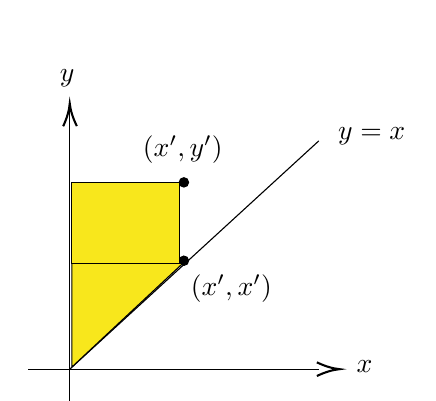
\begin{tikzpicture}[x=0.75pt,y=0.75pt,yscale=-1,xscale=1]
%uncomment if require: \path (0,334); %set diagram left start at 0, and has height of 334

%Straight Lines [id:da6164451716993042] 
\draw    (90,180) -- (230,180) ;
\draw [shift={(240,180)}, rotate = 180] [color={rgb, 255:red, 0; green, 0; blue, 0 }  ][line width=0.75]    (10.93,-3.29) .. controls (6.95,-1.4) and (3.31,-0.3) .. (0,0) .. controls (3.31,0.3) and (6.95,1.4) .. (10.93,3.29)   ;
%Straight Lines [id:da980709989310449] 
\draw    (110,200) -- (110,54) ;
\draw [shift={(110,52)}, rotate = 449.32] [color={rgb, 255:red, 0; green, 0; blue, 0 }  ][line width=0.75]    (10.93,-3.29) .. controls (6.95,-1.4) and (3.31,-0.3) .. (0,0) .. controls (3.31,0.3) and (6.95,1.4) .. (10.93,3.29)   ;
%Straight Lines [id:da9970178018906508] 
\draw    (110,180) -- (230,70) ;
%Shape: Circle [id:dp5087052498778695] 
\draw  [fill={rgb, 255:red, 0; green, 0; blue, 0 }  ,fill opacity=1 ] (162.75,90) .. controls (162.75,88.76) and (163.76,87.75) .. (165,87.75) .. controls (166.24,87.75) and (167.25,88.76) .. (167.25,90) .. controls (167.25,91.24) and (166.24,92.25) .. (165,92.25) .. controls (163.76,92.25) and (162.75,91.24) .. (162.75,90) -- cycle ;
%Shape: Circle [id:dp33272731087373764] 
\draw  [fill={rgb, 255:red, 0; green, 0; blue, 0 }  ,fill opacity=1 ] (167.25,127.66) .. controls (167.3,128.91) and (166.33,129.95) .. (165.09,130) .. controls (163.84,130.05) and (162.8,129.08) .. (162.75,127.84) .. controls (162.7,126.59) and (163.67,125.55) .. (164.91,125.5) .. controls (166.16,125.45) and (167.2,126.42) .. (167.25,127.66) -- cycle ;
%Shape: Right Triangle [id:dp5802057953001984] 
\draw  [color={rgb, 255:red, 0; green, 0; blue, 0 }  ,draw opacity=1 ][fill={rgb, 255:red, 248; green, 231; blue, 28 }  ,fill opacity=1 ] (164.5,129) -- (111,179) -- (111,129) -- cycle ;
%Shape: Rectangle [id:dp40503719241359026] 
\draw  [color={rgb, 255:red, 0; green, 0; blue, 0 }  ,draw opacity=1 ][fill={rgb, 255:red, 248; green, 231; blue, 28 }  ,fill opacity=1 ] (111,90) -- (162.75,90) -- (162.75,129) -- (111,129) -- cycle ;

% Text Node
\draw (247,174.4) node [anchor=north west][inner sep=0.75pt]    {$x$};
% Text Node
\draw (104,34.4) node [anchor=north west][inner sep=0.75pt]    {$y$};
% Text Node
\draw (238,62.4) node [anchor=north west][inner sep=0.75pt]    {$y=x$};
% Text Node
\draw (144,66.4) node [anchor=north west][inner sep=0.75pt]    {$( x',y')$};
% Text Node
\draw (167.09,133.4) node [anchor=north west][inner sep=0.75pt]    {$( x',x')$};

\end{tikzpicture}

    \end{center}
    
    {\color{blue}
    In particular, we see that 
    \[ F(x', y') = \int_0^{x'} \left( \int_x^{y'} f(x, y)\,{\rm d}y \right) {\rm d}x 
    = \int_0^{x'} \left( \int_x^{y'} 2e^{-x-y}\,{\rm d}y \right) {\rm d}x
    = (1-e^{-2x'}) - 2e^{-y'} (1-e^{-x'}). \]
    
    {\sc Case 3.} Suppose that $0 < y' < x'$. We now want to integrate the area below.
    }
    
\begin{center}


\tikzset{every picture/.style={line width=0.75pt}} %set default line width to 0.75pt        

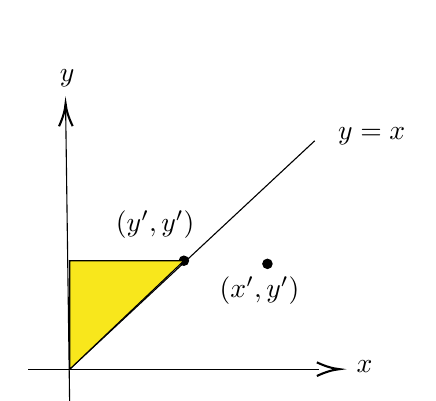
\begin{tikzpicture}[x=0.75pt,y=0.75pt,yscale=-1,xscale=1]
%uncomment if require: \path (0,334); %set diagram left start at 0, and has height of 334

%Straight Lines [id:da6164451716993042] 
\draw    (90,180) -- (230,180) ;
\draw [shift={(240,180)}, rotate = 180] [color={rgb, 255:red, 0; green, 0; blue, 0 }  ][line width=0.75]    (10.93,-3.29) .. controls (6.95,-1.4) and (3.31,-0.3) .. (0,0) .. controls (3.31,0.3) and (6.95,1.4) .. (10.93,3.29)   ;
%Straight Lines [id:da980709989310449] 
\draw    (110,200) -- (108.02,54) ;
\draw [shift={(108,52)}, rotate = 449.32] [color={rgb, 255:red, 0; green, 0; blue, 0 }  ][line width=0.75]    (10.93,-3.29) .. controls (6.95,-1.4) and (3.31,-0.3) .. (0,0) .. controls (3.31,0.3) and (6.95,1.4) .. (10.93,3.29)   ;
%Straight Lines [id:da9970178018906508] 
\draw    (110,180) -- (228,70) ;
%Shape: Circle [id:dp5087052498778695] 
\draw  [fill={rgb, 255:red, 0; green, 0; blue, 0 }  ,fill opacity=1 ] (203,129.25) .. controls (203,128.01) and (204.01,127) .. (205.25,127) .. controls (206.49,127) and (207.5,128.01) .. (207.5,129.25) .. controls (207.5,130.49) and (206.49,131.5) .. (205.25,131.5) .. controls (204.01,131.5) and (203,130.49) .. (203,129.25) -- cycle ;
%Shape: Circle [id:dp33272731087373764] 
\draw  [fill={rgb, 255:red, 0; green, 0; blue, 0 }  ,fill opacity=1 ] (162.75,127.75) .. controls (162.75,126.51) and (163.76,125.5) .. (165,125.5) .. controls (166.24,125.5) and (167.25,126.51) .. (167.25,127.75) .. controls (167.25,128.99) and (166.24,130) .. (165,130) .. controls (163.76,130) and (162.75,128.99) .. (162.75,127.75) -- cycle ;
%Shape: Right Triangle [id:dp5802057953001984] 
\draw  [fill={rgb, 255:red, 248; green, 231; blue, 28 }  ,fill opacity=1 ] (165,127.75) -- (110,180) -- (110,127.75) -- cycle ;

% Text Node
\draw (247,174.4) node [anchor=north west][inner sep=0.75pt]    {$x$};
% Text Node
\draw (104,34.4) node [anchor=north west][inner sep=0.75pt]    {$y$};
% Text Node
\draw (238,62.4) node [anchor=north west][inner sep=0.75pt]    {$y=x$};
% Text Node
\draw (181,134.4) node [anchor=north west][inner sep=0.75pt]    {$( x',y')$};
% Text Node
\draw (131,102.4) node [anchor=north west][inner sep=0.75pt]    {$( y',y')$};

\end{tikzpicture}

\end{center}
    
    {\color{blue}
    Notice that this case simply reduces to Case 2, as we have 
    \[ F(x', y') = F(y', y') = (1-e^{-2y'}) - 2e^{-y'}(1-e^{-y'}) = 1+e^{-2y'} - 2e^{-y'}. \]
    Putting all these together, we have 
    \[ F(x, y) = \begin{cases} 0 & x \leq 0 \text{ or } y \leq 0 \\ 
    (1-e^{-2x}) - 2e^{-y}(1-e^{-x}) & 0 < x \leq y \\ 
    1+e^{-2y} - 2e^{-y} & 0 < y < x. \end{cases} \]
    }
    
    \item Find the marginal CDF of $X$. 
    
    {\color{blue}
    {\bf Solution:} Note that taking $y\to+\infty$, the case $0 < y < x$ is not possible, 
    while the cases $x \leq 0$ and $0 < x \leq y$ are. Namely, we have 
    \[ F_1(x) = \lim_{y\to+\infty} F(x, y) = \begin{cases} 0 & x \leq 0 \\ 1 - e^{-2x} & 
    x > 0. \end{cases} \]
    }
    
\end{enumerate}
\end{exmp}

\subsection{Product rule and independence}

The {\bf product rule} states that if $f(x, y)$ is the joint PF 
(respectively joint PDF) of two discrete (respectively continuous) random variables, then 
\[ f(x, y) = f_1(x \mid y) f_2(y) = f_2(y \mid x) f_1(x). \]
This is immediate from the definition. 

We give an example of applying the product rule. Suppose we are given $f_2(y \mid x)$ and $f_1(x)$, 
and wish to find $f_2(y)$. We can do this with the following steps.
\begin{enumerate}[(i)]
    \item Use the product rule to compute $f(x, y) = f_2(y \mid x) f_1(x)$. 
    \item Compute $f_2(y) = \int_{-\infty}^\infty f(x, y)\,{\rm d}x$ in the continuous case, 
    or $f_2(y) = \sum_{x} f(x, y)$ in the discrete case.
\end{enumerate}

Two random variables $X$ and $Y$ are {\bf independent} if and only if one of the following holds: 
\begin{enumerate}[(1)]
    \item $F(x, y) = F_1(x) F_2(y)$ for all $(x, y) \in \R^2$; 
    \item $f(x, y) = f_1(x) f_2(y)$ for all $(x, y) \in A_1 \times A_2$, where 
    $A_1 = \{x \in \R : f_1(x) > 0\}$ and $A_2 = \{y \in \R : f_2(x) > 0\}$ 
    (the joint support set is rectangular); 
    \item $f_1(x \mid y) = f_1(x)$ for all $x \in A_1$;
    \item $f_2(y \mid x) = f_2(y)$ for all $y \in A_2$;
    \item $M_{(X,Y)}(t_1, t_2) = M_X(t_1) M_Y(t_2)$.
\end{enumerate}

\begin{exmp}
Recall Example 2.7, where we had $(X, Y) \sim \Multi(n, p_1, p_2)$ with joint PF 
\[ f(x, y) = \frac{n!}{x!y!(n-x-y)!} p_1^x p_2^y p_3^{n-x-y}. \]
In particular, we require that $0 \leq x \leq n$, $0 \leq y \leq n$, 
and $0 \leq x+y \leq n$. The condition $0 \leq x+y \leq n$ means that the support set 
is not rectangular (condition (2) fails), and hence $X$ and $Y$ are not independent.
\end{exmp}

\begin{exmp}
From Example 2.8, we had joint PF 
\[ f(x, y) = 2e^{-x-y}, \quad 0 < x < y. \]
Again, this support set is not rectangular, and so $X$ and $Y$ are not independent. 
We can also show this in another way; recall that we had 
\[ f_2(y \mid x) = e^{x-y}, \]
and since this depends on $x$, it cannot be the case that $f_2(y \mid x) = f_2(y)$, 
as $f_2(y)$ does not depend on $x$. Thus, condition (4) above fails.
\end{exmp}

\begin{exmp}
Suppose that $X$ and $Y$ are discrete random variables with joint PF 
\[ f(x, y) = \frac{\theta^{x+y} e^{-2\theta}}{x!y!}, \quad x = 0, 1, 2, \dots, \quad 
y = 0, 1, 2, \dots, \quad \theta > 0. \]
Notice that the support set $A = \Z_{\geq0} \times \Z_{\geq0}$ is rectangular. 
We claim that $X$ and $Y$ are independent. Indeed, we have 
\[ f_1(x) = \sum_{y=0}^\infty f(x, y) = \frac{\theta^x e^{-2\theta}}{x!} \sum_{y=0}^\infty \frac{\theta^y}{y!} = \frac{\theta^x e^{-2\theta}}{x!} \cdot e^\theta = 
\frac{\theta^x}{x!} \cdot e^{-\theta}. \]
In particular, we have $X \sim \Poi(\theta)$. Similarly, one can find that 
\[ f_2(y) = \frac{\theta^y}{y!} \cdot e^{-\theta}, \]
and so $Y \sim \Poi(\theta)$. Since $f(x, y) = f_1(x) f_2(y)$ for all $(x, y) \in A$, 
it follows that $X$ and $Y$ are independent, as claimed.
\end{exmp}

\subsection{Largest and smallest order statistics}

Let $X_1, \dots, X_n$ be a sequence of i.i.d. random variables; that is, a random sample 
from some distribution. We denote the {\bf smallest order statistic} as 
\[ X_{(1)} := \min(X_1, \dots, X_n) \]
and the {\bf largest order statistic} as 
\[ X_{(n)} := \max(X_1, \dots, X_n). \]

Note that we have 
\begin{align*} 
P[X_{(1)} \geq t] &= \prod_{i=1}^n P[X_i \geq t], \\
P[X_{(n)} \leq t] &= \prod_{i=1}^n P[X_i \leq t],
\end{align*} 
as $X_1, \dots, X_n$ are i.i.d. random variables.

Let $X_1, \dots, X_n$ be a random sample of {\it continuous} random variables with CDF 
$F(x)$, pdf $f(x)$, and support set $A$. The PDFs of $X_{(1)}$ and $X_{(n)}$ respectively are 
\begin{align*}
    f_{(1)}(t) &= nf(t)[1-F(t)]^{n-1}, \quad t \in A, \\
    f_{(n)}(t) &= nf(t)[F(t)]^{n-1}, \quad t \in A.
\end{align*}
We prove this for $X_{(1)}$. First, notice that 
\begin{align*}
    P[X_{(1)} \geq t] &= P[X_1 \geq t, X_2 \geq t, \dots, X_n \geq t] \\
    &= \prod_{i=1}^n P[X_i \geq t] \\
    &= \prod_{i=1}^n 1 - P[X_i \leq t] \\
    &= \prod_{i=1}^n 1 - F(t) = (1-F(t))^n. 
\end{align*}
Next, the CDF of $X_{(1)}$ is given by 
\begin{align*}
    F_{(1)}(t) = P(X_{(1)} \leq t) &= 1-P[X_{(1)} > t] 
    = 1-P[X_{(1)} \geq t] 
    = 1-(1-F(t))^n.
\end{align*}
Finally, we see that 
\[ f_{(1)}(t) = \frac{\rm d}{{\rm d}t} F_{(1)}(t) = -n(1-F(t))^{n-1} \cdot \underbrace{(-f(t))}_{(1-F(t))'} = nf(t)[1-F(t)]^{n-1}. \]

\begin{exmp}
Suppose that we have a random sample of size $n$ from $\UNIF(0, \theta)$. Find the PDFs of 
$X_{(1)}$ and $X_{(n)}$. 

{\color{blue}
{\bf Solution:} Let $X_1, \dots, X_n \sim \UNIF(0, \theta)$ be i.i.d. random variables 
where $\theta > 0$. Note that the support set is given by $A = (0, \theta)$. We have CDF 
\[ F(t) = \begin{cases} 0 & t \leq 0 \\ t/\theta & 0 < t < \theta \\ 1 & t \geq \theta. \end{cases} \]
and PDF $f(t) = 1/\theta$, where $t \in (0, \theta)$. Thus, we obtain 
\begin{align*}
    f_{(1)}(t) &= n(1-t/\theta)^{n-1} \cdot 1/\theta, \quad t \in (0, \theta); \\
    f_{(n)}(t) &= n(t/\theta)^{n-1} \cdot 1/\theta, \quad t \in (0, \theta).
\end{align*}}
\end{exmp}

\vspace{-4ex}
\subsection{Sum of independent random variables}

Recall the following facts:
\begin{enumerate}[(1)]
    \item The moment generating function of a random variable $X$ is given by 
    $M_X(t) = E(\exp(tX))$; note that this may not always exist, so we must specify 
    the values of $t$ where it does exist. 
    \item If $X$ and $Y$ are independent, then $M_{(X,Y)}(t_1, t_2) = M_X(t_1) M_X(t_2)$ 
    for all $t_1 \in (-h_1, h_1)$ and $t_2 \in (-h_2, h_2)$, where $h_1, h_2 > 0$.
    \item {\bf Uniqueness Theorem.} Let $X$ and $Y$ be random variables. Then 
    $X$ and $Y$ are identically distributed if and only if $M_X(t) = M_Y(t)$.
\end{enumerate}

\begin{exmp}
Suppose that $X \sim \Nor(\mu_1, \sigma_1^2)$ and $Y \sim \Nor(\mu_2, \sigma_2^2)$ are 
independent. Find the distribution of $X+Y$.

{\color{blue}
    {\bf Solution:} We recall that the moment generating functions of $X$ and $Y$ are given by 
    \begin{align*}
        M_X(t_1) = \exp(t_1 \mu_1 + \tfrac12 t_1^2 \sigma_1^2), \quad t_1 \in \R; \\
        M_Y(t_2) = \exp(t_2 \mu_2 + \tfrac12 t_2^2 \sigma_2^2), \quad t_2 \in \R.
    \end{align*}
    Let us denote $Z = X+Y$. Then 
    \begin{align*}
        M_Z(t) &= E[\exp(tZ)] = E[\exp(t(X+Y))] \\
        &= E[\exp(tX + tY)] = E[\exp(tX) \exp(tY)] \\
        &= E[\exp(tX)] \cdot E[\exp(tY)] \tag{$\star$} \\
        &= M_X(t) M_Y(t) \\ 
        &= \exp(t\mu_1 + \tfrac12 t^2 \sigma_1^2) \exp(t\mu_2 + \tfrac12 t^2 \sigma_2^2) \\
        &= \exp(t(\mu_1+\mu_2) + \tfrac12t^2 (\sigma_1^2 + \sigma_2^2)). 
    \end{align*}
    We justify the equality at $(\star)$. Recall that if $X$ and $Y$ are independent, then 
    $f(x, y) = f_1(x) f_2(y)$ for all $(x, y) \in A= A_1 \times A_2$. In particular, we see that 
    \begin{align*}
        E[h(X) \cdot g(Y)] &= \int_{A_1} \int_{A_2} h(x) g(y) f(x, y)\,{\rm d}x\,{\rm d}y \\
        &= \int_{A_1} \int_{A_2} h(x) g(y) f_1(x) f_2(y)\,{\rm d}x\,{\rm d}y \\
        &= \left( \int_{A_1} h(x) f_1(x) \,{\rm d}x \right) \left( \int_{A_2} g(y) f_2(y)\,{\rm d}y 
        \right) \\
        &= E[h(X)] \cdot E[g(Y)].
    \end{align*}
    Thus, we may conclude that $Z \sim N(\mu_1 + \mu_2, \sigma_1^2 + \sigma_2^2)$. 
    }
\end{exmp}

\begin{exercise}
Suppose that $X \sim \GAM(\alpha_1, \beta)$ and $Y \sim \GAM(\alpha_2, \beta)$ are independent 
random variables. Find the distribution of $X+Y$.
\end{exercise}

\newpage 
\section{Maximum likelihood estimates}

Suppose that $Y \sim f(y; \theta)$. We obtain a random sample $Y_1, 
\dots, Y_n$ (i.i.d.) of size $n$, and denote the observed data by $y_1, \dots, y_n$. 
\begin{enumerate}[(1)]
    \item We know what $f$ is; for example, it could be the PDF of a normal distribution, 
    or the PF of a Poisson distribution.
    \item On the other hand, we do not know what $\theta$ is.
\end{enumerate}
For now, we will focus on {\bf point estimation} of $\theta$ (only one possible 
value of the unknown quantity) as opposed to {\bf set estimation} (such as an interval).
We wish to find $\theta$ based on the observed data $\mathbf{y} = (y_1, \dots, y_n)$. 
We use $\hat\theta$ to denote an estimate of the parameter $\theta$; that is, 
$\hat\theta = \hat\theta(y_1, \dots, y_n) = \hat\theta(\mathbf{y})$.

\begin{defn}
The {\bf likelihood function} (both discrete and continuous cases) for $\theta$ is defined as 
\[ L(\theta) = L(\theta; \mathbf{y}) = \prod_{i=1}^n f(y_i; \theta), \quad \theta \in \Omega, \]
where $\Omega$ is the {\bf parameter space} which contains all possible values of $\theta$. 
\end{defn}

\begin{remark}~
\begin{enumerate}[(1)]
    \item When $Y$ is {\it discrete}, the likelihood function is the probability that we 
    observe the data $\mathbf{y}$, considered as a function of the parameter $\theta$. 
    In particular, $Y_1, \dots, Y_n$ are i.i.d., with $f(y_i; \theta) 
    = P[Y_i = y_i; \theta]$ and 
    \[ L(\theta) = \prod_{i=1}^n P[Y_i = y_i; \theta] = P[Y_1 = y_1, \dots, Y_n = y_n; \theta]. \]
    \item The values of $\theta$ that make the observed data $\mathbf{y}$ more probable 
    would be more credible or likely than those that make the data less probable. 
    \item Hence, taking the largest of such $\theta$ seems like a sensible approach to find the 
    point estimate of $\theta$, and it turns out that it has some very nice properties. 
\end{enumerate}
\end{remark}

\begin{defn}
The value of $\theta$ which maximizes $L(\theta)$ with the observed data $\mathbf{y}$ 
is called the {\bf maximum likelihood estimate (MLE)} of $\theta$. This value is denoted by 
$\hat\theta_{\MLE}$ or just $\hat\theta$; that is, 
\[ \hat\theta_{\MLE} = \hat\theta = \argmax_{\theta\in\Omega} L(\theta). \]
\end{defn}

\begin{remark}~
\begin{enumerate}[(1)]
    \item It is typically easier to work with the log (base $e$) of the likelihood function 
    $L(\theta)$. We denote 
    \[ \ell(\theta) := \log L(\theta). \]
    \item Since functions are often (but not always) maximized by setting their derivatives 
    equal to zero, we can usually obtain $\theta$ by solving the {\bf score equation} 
    \[ \frac{\partial \ell(\theta)}{\partial\theta} = 0. \]
    \item The first derivative test can be used to verify that a solution to 
    $\partial\ell(\theta)/\partial\theta = 0$ corresponds to a maximizer (and not a minimizer). 
    In particular, if $\hat\theta$ is a solution, we need to check that 
    \begin{itemize}
        \item $\partial\ell(\theta)/\partial\theta > 0$ when $\theta < \hat\theta$, and 
        \item $\partial\ell(\theta)/\partial\theta < 0$ when $\theta > \hat\theta$. 
    \end{itemize}
\end{enumerate}
\end{remark}

\begin{exmp}  
During 2016, Nanos Research conducted a survey on Canadian adults to determine support 
for the legalization of marijuana. The 1000 participants were recruited across Canada, 
and were asked "Do you support, somewhat support, somewhat oppose, or oppose legalizing the 
recreational use of marijuana?" 39\% of participants indicated that they supported the 
recreational use of marijuana, while 29\% of participants indicated that they somewhat 
supported it. 

Let $\theta$ denote the proportion of Canadian adults who support or somewhat support the 
recreational use of marijuana. Find the MLE of $\theta$.
\end{exmp}
{\color{blue}
{\bf Solution:} We have $X_1, \dots, X_{1000}$ (i.i.d.) with each $X_i \sim \Ber(\theta)$. 
We have $X_i = 1$ when the recreational use of marijuana is supported or somewhat supported, 
and $X_i = 0$ otherwise. In particular, notice that 
\[ \sum_{i=1}^{1000} X_i \sim \Bin(1000, \theta). \]
Observe that a total of $390 + 290 = 680$ participants from the sample support or somewhat 
support the use of recreational marijuana. This gives 
\[ \sum_{i=1}^{1000} x_i = 680. \] 
Let $Y = \sum_{i=1}^{1000} X_i \sim \Bin(1000, \theta)$, and we have a single observation $y = 680$. 
Then the likelihood function is given by 
\[ L(\theta) = L(\theta; y) = \binom{1000}y \theta^y (1-\theta)^{1000-y}. \]
The log of the likelihood function is then 
\[ \ell(\theta) = \log L(\theta) = \log \binom{1000}y + y\log\theta + (1000-y)\log(1-\theta), \]
and taking the derivative, we get 
\[ \frac{\partial\ell(\theta)}{\partial\theta} = 0 + \frac{y}\theta - \frac{1000-y}{1-\theta} 
= \frac{y(1-\theta) - (100-y)\theta}{\theta(1-\theta)} = \frac{y - 1000\theta}{\theta(1-\theta)}. \]
Solving $\partial\ell(\theta)/\partial\theta = 0$, we have 
\[ \hat\theta = \frac{y}{1000} = \frac{680}{1000} = 0.68. \]
Finally, we use the first derivative test to verify that this is a maximizer. 
\begin{itemize}
    \item If $\theta < \hat\theta = y/1000$, then $1000\theta < y$, which implies that 
    $\partial\ell(\theta)/\partial\theta > 0$. 
    \item If $\theta > \hat\theta = y/1000$, then $1000\theta > y$, so 
    $\partial\ell(\theta)/\partial\theta < 0$.
\end{itemize}
In summary, we obtain $\hat\theta_{\MLE} = \hat\theta = 0.68$. 
}

Recall that to solve $f(x) = 0$ numerically, we can use Newton's method which iteratively computes
\[ x^{(i+1)} = x^{(i)} - \frac{f(x^{(i)})}{f'(x^{(i)})}, \]
and this converges to the solution.

{\bf Newton Raphson method.} To find $\hat\theta$, we usually solve 
$\partial\ell(\theta)/\partial\theta = 0$. When this is not possible 
(there is no explicit solution), we must use numerical methods. 
We can do this using the Newton Raphson method, which is given by 
\[ \theta^{(i+1)} = \theta^{(i)} - \frac{S(\theta^{(i)}; \mathbf{y})}{I(\theta^{(i)}; \mathbf{y})}, \]
where $S(\theta; \mathbf{y}) = \partial\ell(\theta)/\partial\theta$ is the {\bf score function}
and $I(\theta; \mathbf{y}) = -\partial^2\ell(\theta)/\partial\theta^2$ is the 
{\bf information function}. 

Note that in STAT 241, we are not required to carry out the Newton Raphson method (using 
code or other methods). We only need to be able to give the iterative formula above within 
some provided model. 

\newpage 
{\bf Likelihood functions for continuous random variables.} 
Recall that for a continuous random variable $X$, we have $P[X = x; \theta] = 0$ for all 
$x \in \R$. Hence, we need to be more careful than in the discrete case. 

Suppose that $Y$ is a continuous random variable with PDF $f(y; \theta)$. 
We usually observe only the value of $Y$ rounded to some degree of precision; for instance, 
we would round data on waiting time to the nearest second, and data on 
height to the nearest centimeter. 

Suppose we observe $Y = y$ to one decimal place. Then we have 
\[ P[Y = 1.1; \theta] = \int_{1.05}^{1.15} f(y; \theta)\dd y \approx 0.5 \cdot f(1.1; \theta), \]
provided that $f(y; \theta)$ is reasonably smooth between $1.05$ and $1.15$. 

More generally, suppose that $y_1, \dots, y_n$ are the observations from a random sample 
from $f(y; \theta)$ which have been rounded to the nearest $\Delta$ which is assumed 
to be small. Then 
\[ P[\mathbf{Y} = \mathbf{y}; \theta] \approx \prod_{i=1}^n \Delta \cdot f(y_i; \theta) 
= \Delta^n \prod_{i=1}^n f(y_i; \theta). \]
It is a reasonable assumption that the precision $\Delta$ does not depend on the 
unknown parameter $\theta$, so the term $\Delta^n$ can be ignored when finding $\hat\theta$. 
In particular, similarly to the discrete case, we can find $\theta$ by maximizing 
\[ L(\theta) = L(\theta; \mathbf{y}) = \prod_{i=1}^n f(y_i; \theta). \]

{\bf Multiple unknown parameters.} When there are multiple unknown parameters, 
we need to find the MLE by solving multiple equations simultaneously. More explicitly, 
if $\underline\theta = (\theta_1, \dots, \theta_k)$ are unknowns for some $k \geq 1$, then 
we need to solve 
\[ \begin{cases} \partial\ell(\underline\theta)/\partial\theta_1 = 0, \\ \hspace{7ex} \vdots \\ 
\partial\ell(\underline\theta)/\partial\theta_k = 0. \end{cases} \]

{\bf Invariance property of the MLE.} If $\hat\theta$ is the MLE of $\theta$, 
then $g(\hat\theta)$ is the MLE of $g(\theta)$. 

\begin{exmp}
Suppose we want to estimate attributes associated with BMI for some population of individuals. If the distribution of BMI values in the population is well described by a Gaussian model $Y \sim 
\Nor(\mu, \sigma^2)$, then by estimating $\mu$ and $\sigma$, we can estimate any attribute associated with the BMI distribution.

Suppose a random sample of $150$ males gave observations $y_1, \dots, y_{150}$ and 
that the MLEs based on the data are $\hat\mu = 27.1$ and $\hat\sigma = 3.56$. 

\begin{enumerate}[(1)]

    \item Find the median BMI in the population. 
    
    {\color{blue} {\bf Solution:} The median is clearly $\hat\mu = 27.1$.}
    
    \item Find the 10\% quantile of the BMI distribution. 
    
    {\color{blue} {\bf Solution:} Let $\tau$ be the 10\% quantile of $\Nor(\mu, \sigma^2)$. Then 
    \[ 0.1 = P[Y \leq \tau] = P\left[ \frac{Y-\mu}\sigma \leq \frac{\tau-\mu}\sigma \right] 
    = \Phi\left(\frac{\tau-\mu}\sigma\right), \]
    where $\Phi$ is the CDF of $\Nor(0, 1)$. Then we have $(\tau - \mu)/\sigma = -1.28$, 
    which implies that $\tau = \mu - 1.28\sigma$. By the invariance property of the MLE, we 
    then obtain 
    \[ \hat\tau = \hat\mu - 1.28\hat\sigma = 22.54. \]}
    
    \item Find the fraction of the population with BMI over 35.0. 
    
    {\color{blue} {\bf Solution:} Similar to (2), and is left as an exercise (the answer is $0.013$).}
    
\end{enumerate}
\end{exmp}

\newpage 
\section{Expectation-maximization algorithm}

The {\bf expectation-maximization (E-M) algorithm} was popularized by Dempster, Laird, 
and Rubin in 1977 and is a useful method for finding the MLE when (some of) the data 
are incomplete, and can also be applied to other contexts such as mixture models. 

Suppose that 
\begin{itemize}
    \item the complete data $\mathbf X$ has log-likelihood function $\ell(\theta; \mathbf x)$, and 
    \item the incomplete data $\mathbf Y = \mathbf Y(\mathbf X)$ has log-likelihood function 
    $\ell^*(\theta; \mathbf y)$. 
\end{itemize}
Usually, maximizing $\ell(\theta; \mathbf x)$ is easier than maximizing $\ell^*(\theta; \mathbf y)$. 
However, suppose that we can only observe $\mathbf Y = \mathbf y$, while 
$\mathbf X = \mathbf x$ (and hence $\ell(\theta; \mathbf x)$) is unavailable. 

The E-M algorithm uses an iterative two-step method. We denote by $\theta^{(k)}$ the 
estimate of $\theta$ at the $k$-th iteration of the algorithm. 

{\bf Step 0.} Choose an initial value $\theta^{(0)}$ based on the complete part of the incomplete 
data. Usually, if $\mathbf Y = (Y_1, \dots, Y_n)$ is the incomplete data and 
$(Y_1, \dots, Y_j)$ is the complete part of the incomplete data, 
then it is reasonable to set 
\[ \theta^{(0)} = \frac{1}{j} \sum_{i=1}^j y_i. \]
{\bf Step 1.} This is the first step of the two-step method, the {\bf E-step}. We find 
\[ Q(\theta, \theta^{(k)}) := E[\ell(\theta; \mathbf X) \mid \mathbf Y = \mathbf y; \theta^{(k)}]. \]
{\bf Step 2.} This is the second step of the two-step method, the {\bf M-step}. We let 
\[ \theta^{(k+1)} = \max_\theta Q(\theta, \theta^{(k)}). \]
Note that the $\max$ is with respect to $\theta$, and not $\theta^{(k)}$. We can 
do this similarly to the usual method; solve $\partial Q(\theta, \theta^{(k)})/\partial\theta = 0$
and apply the first derivative test. 

{\bf Step 3.} We check for convergence. In particular, we verify that 
\[ |\theta^{(k+1)} - \theta^{(k)}| < \varepsilon \]
for some chosen tolerance level $\varepsilon > 0$. If not, go back to Step 1. 

In Step 1, it is useful to note that if $\mathbf X = (X_1, \dots, X_n)$ are independent, then  
$\mathbf Y(\mathbf X) = (Y_1, \dots, Y_n)$ is also independent. Moreover, we have that 
\[ E[x_i \mid \mathbf Y = \mathbf y; \theta^{(k)}] = E[x_i \mid Y_i = y_i; \theta^{(k)}]. \]
Indeed, we can verify this for the special case $n = 2$ which can then be generalized. 
Suppose that $X_1$ is independent of $X_2$. Then $Y_1$ and $Y_2$ are also 
independent. Also, we have 
\[ f(x_1 \mid y_1, y_2) = \frac{f(x_1, y_1, y_2)}{f(y_1, y_2)} = 
\frac{f(x_1, y_1 \mid y_2)f(y_2)}{f(y_1 \mid y_2)f(y_2)} = \frac{f(x_1, y_1)}{f(y_1)} = f(x_1 \mid y_1), \]
where the second equality is by the product rule, and the third equality follows from independence. 

\newpage 
\section{Sampling distributions}

To investigate properties of estimates, we note that our estimate $\hat\theta = \hat\theta(\mathbf y)$ 
depends on the observed sample $\mathbf Y = \mathbf y$. In particular, if we take different 
samples $\mathbf y^1, \dots, \mathbf y^M$ where 
\[ \mathbf y^j = (y_1^j, \dots, y_{n_j}^j) \] 
and $n_j$ is the sample size of $\mathbf y^j$, then we obtain different estimates 
$\hat\theta_1 = \hat\theta(\mathbf y^1)$, $\dots$, $\hat\theta_M = \hat\theta(\mathbf y^M)$. 

Moreover, we can think of each estimate $\hat\theta(\mathbf y)$ as a realization of a random variable 
$\hat\theta(\mathbf Y)$, which has its own distribution, mean, and variance, among other properties.

How close to $\theta$ could we expect $\hat\theta(\mathbf Y)$ to be? How do we quantify the 
uncertainty in $\hat\theta(\mathbf Y)$? To answer these questions, we introduce estimators 
and sampling distributions. 

\begin{defn}
A {\bf point estimator} is a random variable which is a function $\hat\theta(\mathbf Y)$ of a random 
sample $\mathbf Y = (Y_1, \dots, Y_n)$. 
\end{defn}

Note that a {\bf point estimate} $\hat\theta(\mathbf y)$ is the value of this function 
$\hat\theta(\cdot)$ based on a particular observed sample $\mathbf y = (y_1, \dots, y_n)$. 

\begin{defn}
The distribution of an estimator $\hat\theta(\mathbf Y)$ is called the {\bf sampling distribution} 
of the estimator. 
\end{defn}

\begin{remark}
Observe that $\hat\theta(\mathbf Y)$ is random as the sample $\mathbf Y$ is random. 
Consequently, $\hat\theta(\mathbf y)$ is a realization of $\hat\theta(\mathbf Y)$ since 
$\mathbf y$ is a realization of $\mathbf Y$. 
\end{remark}

\begin{exmp}
Suppose that $(Y_1, \dots, Y_n)$ is a random sample from $\Nor(\mu, \sigma^2)$. 
Find the sampling distribtuion of $\hat\mu(\mathbf Y) = \overline Y = \frac1n \sum_{i=1}^n Y_i$. 
\end{exmp}
{\color{blue}
{\bf Solution:} 
Recall that in Week 1, we derived the moment generating function of $Y \sim \Nor(\mu, \sigma^2)$, 
which is given by 
\[ M_Y(t) = \exp\left(t\mu + \frac12 t^2 \sigma^2\right), \quad t \in \R. \]
Moreover, recall that $X$ and $Y$ are independent if and only if $M_X(t_1) \cdot M_Y(t_2) 
= M_{(X,Y)}(t_1, t_2)$ for all $t_1 \in (-h_1, h_1)$ and $t_2 \in (-h_2, h_2)$ for some 
$h_1, h_2 > 0$. 

Therefore, since $(Y_1, \dots, Y_n)$ are independent, we have 
\begin{align*}
    M_{(Y_1, \dots, Y_n)}(t_1, \dots, t_n) 
    &= E [ \exp(t_1Y_1 + t_2Y_2 + \cdots + t_nY_n) ] \\
    &= E [ \exp(t_1 Y_1) ] E [ \exp(t_2 Y_2) ] \cdots E [ \exp(t_n Y_n) ] \\
    &= M_{Y_1}(t_1) M_{Y_2}(t_2) \cdots M_{Y_n}(t_n) \\
    &= \prod_{i=1}^n M_{Y_i}(t_i) \\
    &= \prod_{i=1}^n M_Y(t_i) \\
    &= \prod_{i=1}^n \exp \left(t_i \mu + \frac12 t_i^2 \sigma^2 \right) \\
    &= \exp \left( \mu \sum_{i=1}^n t_i + \frac12 \sigma^2 \sum_{i=1}^n t_i^2 \right). 
\end{align*}
\newpage 
Now, note that we are trying to find the moment generating function of 
$\hat\mu(\mathbf Y) = \frac1n \sum_{i=1}^n Y_i$, which we will denote by $M(t)$. We have 
\begin{align*}
    M(t) &= 
    E [ \exp(t \cdot \hat\theta(\mathbf Y)) ] \\
    &= E \left[ \exp \left( t \cdot \frac1n \sum_{i=1}^n Y_i \right) \right] \\
    &= E \left[ \exp \left( \frac tn \cdot Y_1 + \frac tn \cdot Y_2 + \cdots + \frac tn Y_n \right)
    \right] \\
    &= M_{(Y_1, \dots, Y_n)}\left( \frac tn, \frac tn, \dots, \frac tn \right) \\
    &= \exp \left( \mu \sum_{i=1}^n \frac tn + \frac12 \sigma^2 \sum_{i=1}^n \left( \frac tn \right)^2 
    \right) \\
    &= \exp \left( \mu t + \frac12 \sigma^2 \frac{t^2}n \right).
\end{align*}
Observe that this is the moment generating function of $\Nor(\mu, \sigma^2/n)$. 
Due to the Uniqueness Theorem of moment generating functions, it follows that 
\[ \hat\mu(\mathbf Y) = \overline Y \sim \Nor(\mu, \sigma^2/n). \]}

\vspace{-3ex}
\begin{exmp}
Suppose that $(Y_1, \dots, Y_n)$ is a random sample from $\EXP(\theta)$. Find the 
sampling distribution of $\hat\theta(\mathbf Y) = \overline Y = \frac1n \sum_{i=1}^n Y_i$. 
\end{exmp}
{\color{blue}
{\bf Solution:} 
Recall that the PDF of $Y \sim \EXP(\theta)$ is given by 
\[ f(y; \theta) = \frac1\theta \exp \left( - \frac y\theta \right), \quad y > 0, \quad \theta > 0. \]
Then, we see that 
\begin{align*}
    M_Y(t) = E[\exp(t \cdot Y)] &= \int_0^\infty \exp(t \cdot y) \cdot \frac1\theta \exp\left( 
    -\frac y\theta \right)\dd y \\
    &= \frac1\theta \int_0^\infty \exp\left( \left(t - \frac1\theta \right)y \right) \dd y & \tag{$\star$} \\
    &= \frac1\theta \cdot \frac1{t-1/\theta} \left[ \exp \left( \left(t - \frac1\theta \right)y \right) 
    \right]_{y=0}^{y\to\infty} \\
    &= \frac1\theta \cdot \frac1{t-1/\theta} [0 - 1] \\
    &= \frac1{1-\theta t}, \quad t < \frac1\theta. 
\end{align*}
Note that $M_Y(t)$ only exists for $t < 1/\theta$ as the integral at $(\star)$ is finite only
when $t - 1/\theta < 0$. 

Now, the moment generating function of $\overline Y = \frac1n \sum_{i=1}^n Y_i$ is 
\begin{align*}
    M(t) &= E\left[ \exp \left(t \cdot \frac1n \sum_{i=1}^n Y_i \right) \right] \\
    &= E \left[ \exp \left( \frac tn \cdot Y_1 + \cdots + \frac tn \cdot Y_n \right) \right] \\
    &= \prod_{i=1}^n M_y \left( \frac tn \right) \\
    &= \prod_{i=1}^n \frac{1}{1-\theta \cdot t/n} \\
    &= \left( \frac{1}{1- \theta \cdot t/n} \right)^n, \quad \frac tn < \frac1\theta.
\end{align*}
As an exercise, verify that if $X \sim \GAM(\alpha, \beta)$, then the moment generating function of 
$X$ is 
\[ M_X(t) = \frac{1}{(1-\beta t)^\alpha}, \quad t < \frac1\beta. \]
In particular, we see that $M(t)$ is the moment generating function of $\GAM(n, \theta/n)$. 
By the Uniqueness Theorem of moment generating functions, we have 
\[ \hat\theta(\mathbf Y) = \overline Y \sim \GAM(n, \theta/n). \]
}

\vspace{-3ex}
Now, suppose we have a random sample $(Y_1, \dots, Y_n)$ from $\Poi(\theta)$, and we wish to 
find the sampling distribution of $\hat\theta(\mathbf Y) = \overline Y = \frac1n \sum_{i=1}^n Y_i$. 

As usual, we start by finding the moment generating function of $Y \sim \Poi(\theta)$; as 
an exercise, we can find that 
\[ M_y(t) = e^{\theta(e^t-1)}, \quad t \in \R. \] 
Then, for $\hat\theta(\mathbf Y) = \overline Y$, the moment generating function is given by 
\[ M(t) = \prod_{i=1}^n M_Y \left( \frac tn \right) = \prod_{i=1}^n e^{\theta(e^{t/n}-1)} 
= e^{n\theta(e^{t/n}-1)}, \quad t \in \R. \]
What random variable has this moment generating function? This is certainly not a Poisson distribution 
due to the $t/n$ term. In fact, this is not any of the commonly seen random variables. Hence, 
we cannot apply the same techniques which we used in Example 5.4 and Example 5.5.

This shows us that the sampling distribution often has to be determined approximately, using 
results such as the Central Limit Theorem. 

\begin{thm}[Central Limit Theorem]
Suppose that $(Y_1, \dots, Y_n)$ is a random sample with $E(Y_i) = \mu$ and 
$\Var(Y_i) = \sigma^2 < \infty$. Then, we have 
\[ \frac{\sqrt n (\overline Y - \mu)}{\sigma} \sim \Nor(0, 1) \]
approximately/for large $n$.
\end{thm}

Note that larger $n$ or smaller $\sigma$ results in a smaller approximation 
$\Var(\overline Y)$, which means that our estimate is more likely to be close to the true value 
$\mu$ (estimated by $\overline Y$).

Let us consider how we can apply the Central Limit Theorem to our situation. 
Suppose that $Z = \sqrt n(\overline Y - \mu)/\sigma \sim \Nor(0, 1)$ approximately/for large $n$. 
Then, by the Central Limit Theorem, we have
\[ M_Z(t) \approx \exp \left(t \cdot 0 + \frac12 t^2 \cdot 1 \right) = \exp \left( \frac12 t^2 \right). \]
Consequently, we obtain 
\begin{align*}
    M_{\overline Y}(t) &= E[\exp(t \cdot \overline Y)] \\
    &= E \left[ \exp \left( t \cdot \left( \frac{\sigma Z}{\sqrt n} + \mu \right) \right) \right] \\
    &= \exp(t\mu) \cdot E \left[ \exp \left( \frac{t\sigma}{\sqrt n} \cdot Z \right) \right] \\
    &\approx \exp(t\mu) \cdot \exp \left( \frac12 \left( \frac{t\sigma}{\sqrt n} \right)^2 \right) \\
    &= \exp \left( t\mu + \frac12 t^2 \frac{\sigma^2}n \right),
\end{align*}
where we have the approximation since $E [ \exp(t\sigma / \sqrt n \cdot Z)]$ is the moment 
generating function of $Z$ applied at $t\sigma / \sqrt n$. In particular, this is the 
moment generating function of $\Nor(\mu, \sigma^2/n)$, so we have 
$\overline Y \sim \Nor(\mu, \sigma^2/n)$ approximately/for large $n$. 

\begin{remark}
The variation $\sigma^2/n$ of $\overline Y$ is small (which is desirable) when $\sigma$ is small 
or $n$ is large. 
\end{remark}

It is important to note that we only have an approximate sampling distribution when doing this.
We now take a look at Markov's Inequality and Chebyshev's Inequality to help us quantify how good these 
approximations are. 

\begin{thm}[Markov's Inequality]
For any random variable $X$ such that $E(|X|^k)$ is finite, we have 
\[ P( |X| \geq c ) \leq \frac{E (|X|^k|)}{c^k} \]
for all $c > 0$ and $k > 0$. We often call $P(|X| \geq c)$ the {\bf tail probability}.
\end{thm}
\begin{pf}
We prove Markov's Inequality in the case where $X$ is a continuous random variable; the 
proof is similar in the discrete case by replacing the integral with the summation. 
Indeed, for all $c > 0$ and $k > 0$, we have 
\begin{align*}
    \frac{E (|X|^k|)}{c^k} 
    &= E \left[ \left( \frac{|x|}c \right)^k \right] \\
    &= E \left [ \left| \frac xc \right|^k \right] \\
    &= \int_{-\infty}^\infty \left| \frac xc \right|^k f(x)\dd x \\
    &= \int_{\{x : |x/c| \geq 1\}} \left| \frac xc \right|^k f(x) \dd x 
    + \int_{\{x : |x/c| < 1\}} \left| \frac xc \right|^k f(x) \dd x \\
    &\geq \int_{\{x : |x/c| \geq 1\}} \left| \frac xc \right|^k f(x) \dd x \\
    &\geq \int_{\{x : |x/c| \geq 1\}} f(x) \dd x \\
    &= \int_{\{x : |x| \geq c\}} f(x) \dd x 
    = P(|X| \geq c). \qedhere 
\end{align*}
\end{pf}

\begin{thm}[Chebyshev's Inequality]
For any random variable $X$ such that $E(X) = \mu$ and $\Var(X) = \sigma^2$ are finite, we have 
\[ P(|X - \mu| \geq \beta\sigma) \leq \frac1{\beta^2} \]
for all $\beta > 0$.
\end{thm}
\begin{pf}
Let $Y = X - \mu$. Then $E(Y) = 0$ and $\Var(Y) = \Var(X) = \sigma^2$. Let $\beta > 0$. 
By Markov's Inequality, for all $k > 0$, we have 
\[ P(|Y| \geq \beta\sigma) \leq \frac{E(|Y|^k)}{(\beta\sigma)^k}. \]
In particular, for $k = 2$, it follows that 
\[ P(|Y| \geq \beta\sigma) \leq \frac{E(Y^2)}{(\beta\sigma)^2} 
= \frac{E[(X-\mu)^2]}{\beta^2\sigma^2} = \frac{\Var(X)}{\beta^2\sigma^2} = 
\frac{\sigma^2}{\beta^2\sigma^2} = \frac{1}{\beta^2}. \qedhere \]
\end{pf}

We can now return to the example where we could not find an exact sampling distribution. 

\begin{exmp}
Suppose that $(Y_1, \dots, Y_n)$ is a random sample from $\Poi(\theta)$. Find the approximate
sampling distribution of $\hat\theta(\mathbf Y) = \overline Y = \frac1n \sum_{i=1}^n Y_i$. 
\end{exmp}
{\color{blue}
{\bf Solution:} 
Note that we have $E(Y_i) = \Var(Y_i) = \theta < \infty$. Then by the Central Limit Theorem, we have 
\[ Z = \frac{\sqrt n(\overline Y - E(Y_i))}{\sqrt{\Var(Y_i)}} 
= \frac{\sqrt n(\overline Y - \theta)}{\sqrt\theta} \sim \Nor(0, 1) \]
approximately/for large $n$. Then $M_Z(t) \approx \exp(\frac12 t^2)$, and hence 
\begin{align*}
    M_{\overline Y}(t) 
    &= E \left[ \exp\left(t \cdot \frac{\sqrt\theta \cdot Z}{\sqrt n} + \theta \right) \right] \\
    &= \exp(t\theta) \cdot E \left[ \exp \left( \frac{t\sqrt\theta}{\sqrt n} \cdot Z \right) \right] \\
    &\approx \exp(t\theta) \cdot \exp \left( \frac12 \cdot \frac{t^2\theta}n \right) \\
    &= \exp\left( t\theta + \frac12 t^2 \cdot \frac\theta n \right). 
\end{align*}
This is the moment generating function of $\Nor(\theta, \theta/n)$, so we have 
$\overline Y \sim \Nor(\theta, \theta/n)$, approximately. 

We now use Chebyshev's Inequality to discuss how close $\overline Y$ is to the true value of 
$\theta$. Indeed, for all $\beta > 0$, we have (approximately)
\[ P\left(|\overline Y - \theta| \geq \beta \cdot \sqrt{\theta/n} \right) \leq \frac1{\beta^2}. \]
Let the sample size be $n = 81$, that is, $\overline{Y}_{81} = \frac1{81} \sum_{i=1}^{81} Y_i$. 
Choose $\beta = 3$. Then 
\[ P\left(|\overline Y_{81} - \theta| \geq 3 \cdot \sqrt{\theta/81} \right)
= P\left(|\overline Y_{81} - \theta| \geq \frac13 \sqrt{\theta} \right) \leq \frac19, \]
which implies that 
\[ P\left(|\overline Y_{81} - \theta| \leq \frac13 \sqrt{\theta} \right) \geq 1 - \frac19
= \frac89. \]
Similarly, taking $n = 49$, we obtain 
\[ P\left(|\overline Y_{49} - \theta| \leq \frac37 \sqrt{\theta} \right) \geq \frac89. \]
Clearly we have $\frac13\sqrt\theta < \frac37\sqrt\theta$, so $\overline Y_{81}$ is more likely 
to be close to the true value of $\theta$. 
}

\newpage 
\section{Unbiased estimators and the Cramer-Rao lower bound}

\begin{defn}[Bias]
The {\bf bias} of an estimator $\hat\theta(\mathbf Y)$ is given by 
\[ \Bias(\hat\theta) = E(\hat\theta) - \theta. \]
If the bias equals $0$, then the estimator is said to be {\bf unbiased}.
\end{defn}

Intuitively, an unbiased estimator will be correct "on average". Moreover, if we have multiple 
unbiased estimators, we ideally want to choose the one with the smallest variance, 
as smaller variance leads to estimates that are closer to the true value of $\theta$. 

What happens if we do not have unbiased estimators? Also, if we have an unbiased estimator 
with high variance and a biased estimator with low variance, which one do we choose?

\begin{defn}[Mean squared error]
The {\bf mean squared error (MSE)} of an estimator is given by 
\[ \MSE(\hat\theta) = E[(\hat\theta - \theta)^2]. \]
\end{defn}

\begin{thm}
We have $\MSE(\hat\theta) = E[(\hat\theta - \theta)^2] = \Var(\hat\theta) + (\Bias(\hat\theta))^2$. 
\end{thm}
\begin{pf}
Observe that 
\begin{align*}
    \MSE(\hat\theta) &= E[(\hat\theta - \theta)^2] \\
    &= E[(\hat\theta - E(\hat\theta) + E(\hat\theta) - \theta)^2] \\
    &= E[(\hat\theta - E(\hat\theta))^2 + (E(\hat\theta) - \theta)^2 + 
    2(\hat\theta - E(\hat\theta))(E(\hat\theta) - \theta)] \\
    &= E[(\hat\theta - E(\hat\theta))^2] + E[(E(\hat\theta) - \theta)^2] 
    + 2E[(\hat\theta - E(\hat\theta)(E(\hat\theta) - \theta)] \\
    &= \Var(\hat\theta) + E[(\Bias(\hat\theta))^2] + 2(E(\hat\theta) - \theta) (E(\hat\theta) 
    - E(E(\hat\theta))) \\
    &= \Var(\hat\theta) + (\Bias(\hat\theta))^2. \qedhere 
\end{align*}
\end{pf}

\begin{remark}~
\begin{enumerate}[(i)]
    \item Large variance and bias are both undesirable. We compute the MSE to strike a 
    balance between these two quantities. 
    \item If an estimator is unbiased, then the MSE is simply the variance of the estimator. 
\end{enumerate}
\end{remark}

\begin{exmp}
Suppose that $X_1, \dots, X_n$ is a random sample from $\UNIF(0, \theta)$. Compare the 
MSEs of the three estimators $2\bar{X}$, $X_{(n)}$, and $(n+1)X_{(1)}$ for $\theta$. 
\end{exmp}
{\color{blue}
{\bf Solution:} 
Let $T_1 = 2\bar{X}$, $T_2 = X_{(n)}$, and $T_3 = (n+1)X_{(1)}$. For each $1 \leq i \leq 3$, we need 
to find $\Var(T_i)$ and $E(T_i)$ in order to comptute $\MSE(T_i)$. 
\begin{enumerate}[(1)]
    \item For $T_1 = 2\bar{X}$, we have 
    \[ E(T_1) = 2E[\bar{X}] = 2E\left( \frac1n \sum_{i=1}^n X_i \right) = \frac{2n E[X_1]}n 
    = 2 \cdot \frac\theta2 = \theta. \]
    It follows that $\Bias(T_1) = E(T_1) - \theta = 0$, so $T_1$ is unbiased. Moreover, we obtain 
    \[ \Var(T_1) = \Var(2\bar{X}) = 4\Var\left(\frac1n \sum_{i=1}^n X_i \right) = 
    \frac4{n^2} \sum_{i=1}^n \Var(X_i) = \frac4n \Var(X_1) = \frac4n \cdot \frac{\theta^2}{12} = 
    \frac{\theta^2}{3n}. \]
    Finally, we get 
    \[ \MSE(T_1) = \frac{\theta^2}{3n} + 0^2 = \frac{\theta^2}{3n}. \]
    \item Recall that $X \sim \UNIF(0, \theta)$ has PDF $f(x) = 1/\theta$ for $0 \leq x \leq \theta$ 
    and CDF given by 
    \[ F(x) = \begin{cases} 0 & x < 0, \\ x/\theta & 0 \leq x \leq \theta, \\ 1 & x \geq \theta.
    \end{cases} \]
    Hence, the PDF of $T_2 = X_{(n)}$ is 
    \[ f_{T_2}(t) = nf(t)(F(t))^{n-1} = n \cdot \frac1\theta \cdot \left( \frac t\theta\right)^{n-1}
    = \frac{nt^{n-1}}{\theta^n}, \quad 0 \leq t \leq \theta. \]
    Now, we obtain 
    \[ E(T_2) = \int_0^\theta t \cdot \frac{nt^{n-1}}{\theta^n}\dd t = \frac{n}{n+1}\theta, \]
    and we see that $T_2$ is biased. Similarly, we have 
    \[ E(T_2^2) = \int_0^\theta t^2 \cdot \frac{nt^{n-1}}{\theta^n}\dd t = 
    \frac{n}{\theta^n} \cdot \frac{\theta^{n+2}}{n+2} = \frac{n}{n+2} \theta^2, \]
    so it follows that 
    \[ \Var(T_2) = E(T_2^2) - (E(T_2))^2 = \frac{n\theta^2}{(n+2)(n+1)^2}. \]
    Finally, we get 
    \[ \MSE(T_2) = \frac{n\theta^2}{(n+2)(n+1)^2} = \left( \frac{n}{n+1}\theta - \theta \right)^2 
    = \frac{2\theta^2}{(n+1)(n+2)}. \]
    \item Recall that the PDF of $X_{(1)}$ is given by 
    \[ f_{X_{(1)}}(t) = nf(t)[1 - F(t)]^{n-1}, \quad 0 \leq x \leq \theta. \]
    We leave it as an exercise to show that 
    \[ \MSE(T_3) = \frac{n}{n+2}\theta^2. \]
\end{enumerate}
Putting these together, we have 
\begin{align*}
    \MSE(T_1) &= \frac{\theta^2}{3n}, &
    \MSE(T_2) &= \frac{\theta^2}{(n+1)(n+2)/2}, &
    \MSE(T_3) &= \frac{\theta^2}{(n+2)/n}. 
\end{align*}
To compare the MSEs, it suffices to look at the denominators. Indeed, note that 
$3n \geq (n+2)/n$ for all $n \geq 1$, and $3n \leq (n+1)(n+2)/2$ for all $n \geq 1$, so 
we can conclude that 
\[ \MSE(T_2) \leq \MSE(T_1) \leq \MSE(T_3). \]}

\begin{thm}[Cramer-Rao lower bound]
Suppose that $\mathbf{X} = (X_1, \dots, X_n)$ is a random sample from $f(x; \theta)$. 
Denote $J(\theta) = E[I(\theta; \mathbf{X})]$, where 
\[ I(\theta; \mathbf{x}) = -\frac{\partial}{\partial\theta} S(\theta; \mathbf{x}) = 
- \frac{\partial^2}{\partial\theta^2} \ell(\theta; \mathbf{x}). \]
We call $J(\theta)$ the {\bf Fisher information}. For any {\it unbiased} estimator 
$T(\mathbf X)$ of $\tau(\theta)$ (which is a function of $\theta$ we wish to examine), 
its variance has the lower bound 
\[ \Var[T(\mathbf X)] \geq \frac{[\tau'(\theta)]^2}{J(\theta)}, \]
where $\tau'(\theta) = d\tau(\theta)/d\theta$. 
\end{thm}
\begin{pf}
We will make use of the Cauchy-Schwarz inequality which is given by 
\[ \Cov^2(X, Y) \leq \Var(X) \cdot \Var(Y), \]
as well as the following claims. 

{\sc Claim 1.} We have $E[S(\theta; \mathbf{X})] = 0$. 

{\sc Proof of Claim 1.} We prove this in the continuous case; the discrete case is analogous. We have 
\begin{align*}
    E\left[ \frac{\partial}{\partial\theta} \ell(\theta; \mathbf X) \right] 
    &= \int \frac{\partial}{\partial\theta} \ell(\theta; \mathbf x) \cdot L(\theta; \mathbf x)
    \dd \mathbf x \\
    &= \int \frac{\partial}{\partial\theta} \log L(\theta; \mathbf x) \cdot L(\theta; \mathbf x)
    \dd \mathbf x \\
    &= \int \frac{\frac{\partial}{\partial\theta} L(\theta; \mathbf x)}{L(\theta; \mathbf x)} \cdot L(\theta; \mathbf x) \dd \mathbf x \\
    &= \int \frac{\partial}{\partial\theta} L(\theta; \mathbf x) \dd \mathbf x \\
    &= \frac{\partial}{\partial\theta} \int  L(\theta; \mathbf x) \dd \mathbf x \\
    &= \frac{\partial}{\partial\theta} 1 = 0. \tag*{$\blacksquare$}
\end{align*}
{\sc Claim 2.} We have $J(\theta) = \Var(\frac{\partial}{\partial\theta} \ell(\theta; 
\mathbf X))$. 

{\sc Proof of Claim 2.} Note that 
\[ J(\theta) = E[I(\theta; \mathbf X)] = E\left[ -\frac{\partial^2}{\partial \theta^2} \ell(\theta;
\mathbf X) \right]. \]
By Claim 1, we have $E[\frac{\partial}{\partial\theta} \ell(\theta; \mathbf X)] = 0$, so it follows that 
\[ \Var\left[ \frac{\partial}{\partial\theta} \ell(\theta; \mathbf X) \right] = 
E \left[ \left( \frac{\partial}{\partial\theta} \ell(\theta; \mathbf X) \right)^2 \right]. \]
Therefore, to prove the claim, it suffices to show that 
\[ E\left[ -\frac{\partial^2}{\partial \theta^2} \ell(\theta;
\mathbf X) \right] = E \left[ \left( \frac{\partial}{\partial\theta} \ell(\theta; \mathbf X) \right)^2 \right]. \]
Indeed, we have 
\begin{align*}
    E\left[ -\frac{\partial^2}{\partial \theta^2} \ell(\theta;
\mathbf X) \right] 
&= \int \left( -\frac{\partial^2}{\partial\theta^2} \ell(\theta; \mathbf x) \right) \cdot L(\theta; 
\mathbf x)\dd\mathbf x \\
&= \int -\frac{\partial}{\partial\theta} \left( \frac{\partial}{\partial\theta} \log L(\theta;
\mathbf x) \right) \cdot L(\theta; \mathbf x) \dd\mathbf x \\
&= \int - \frac{\partial}{\partial\theta} \frac{L'(\theta; \mathbf x)}{L(\theta; \mathbf x)} 
\cdot L(\theta; \mathbf x) \dd\mathbf x \\
&= \int - \frac{L''(\theta; \mathbf x) \cdot L(\theta; \mathbf x) - (L'(\theta; \mathbf x))^2}{(L(\theta; \mathbf x))^2} \cdot L(\theta; \mathbf x)\dd\mathbf x \\
&= \int - \left( L''(\theta; \mathbf x) - \frac{(L'(\theta; \mathbf x))^2}{L(\theta; \mathbf x)} \right)\dd\mathbf x \\
&= \int \frac{(L'(\theta; \mathbf x))^2}{L(\theta; \mathbf x)} \dd\mathbf x - \int 
\frac{\partial^2}{\partial\theta^2} L(\theta; \mathbf x)\dd \mathbf x \\
&= \int \left( \frac{L'(\theta; \mathbf x)}{L(\theta; \mathbf x)} \right)^2 \cdot L(\theta; 
\mathbf x) \dd\mathbf x 
= \int \left( \frac{\partial}{\partial\theta} \ell(\theta; \mathbf x) \right)^2 \cdot L(\theta; 
\mathbf x) \dd \mathbf x = E \left[ \left( \frac{\partial}{\partial\theta} \ell(\theta; \mathbf X) 
\right)^2 \right]. \tag*{$\blacksquare$}
\end{align*}
Now, we show that $\tau'(\theta) = \Cov(T(\mathbf X), S(\theta; \mathbf X))$. Indeed, recall that 
\[ \tau(\theta) = E[T(\mathbf X)] = \int T(\mathbf x) \cdot L(\theta; \mathbf x)\dd\mathbf x. \]
Then we have 
\begin{align*}
    \tau'(\theta) = \frac{\rm d}{{\rm d}\theta} \tau(\theta)
    &= \frac{\rm d}{{\rm d}\theta} \int T(\mathbf x) \cdot L(\theta; \mathbf x)\dd\mathbf x \\
    &= \int \frac{\partial}{\partial\theta} (T(\mathbf x) \cdot L(\theta; \mathbf x)) \dd\mathbf x \\
    &= \int T(\mathbf x) \cdot \frac{\partial}{\partial\theta} L(\theta; \mathbf x) \dd \mathbf x \\
    &= \int T(\mathbf x) \cdot \frac{\frac{\partial}{\partial\theta} L(\theta; \mathbf x)}{L(\theta; \mathbf x)} \cdot L(\theta; \mathbf x) \dd \mathbf x \\
    &= \int T(\mathbf x) \cdot \frac{\partial}{\partial\theta} \ell(\theta; \mathbf x) 
    \cdot L(\theta; \mathbf x) \dd \mathbf x \\
    &= E[T(\mathbf X) \cdot S(\theta; \mathbf X)] \\
    &= E[T(\mathbf X) \cdot S(\theta; \mathbf X)] - E[T(\mathbf X)] E[S(\theta; \mathbf X)] \\
    &= \Cov(T(\mathbf X), S(\theta; \mathbf X)). 
\end{align*}
We note that in the second last step, we use the fact that $E[S(\theta; \mathbf X)] = 0$ from 
Claim 1. Finally, by the Cauchy-Schwarz inequality, we obtain 
\[ \Var[T(\mathbf X)] \cdot J(\theta) = \Var[T(\mathbf X)] \cdot 
\Var[S(\theta; \mathbf X)] \geq \Cov^2(T(\mathbf X), S(\theta; \mathbf X)) = (\tau'(\theta))^2, \]
which is exactly what we needed to prove. 
\end{pf}

\begin{defn}[Efficiency]
The ratio of the Cramer-Rao lower bound to the variance of an unbiased estimator $T(\mathbf X)$ is 
called the {\bf efficiency} of the estimator; that is, 
\[ \Eff(T(\mathbf X)) = \frac{(\tau'(\theta))^2/J(\theta)}{\Var(T(\mathbf X))}. \]
Note that $0 \leq \Eff(T(\mathbf X)) \leq 1$. If $\Eff(T(\mathbf X)) = 1$, then $T(\mathbf X)$ 
attains the Cramer-Rao lower bound, and we call $T(\mathbf X)$ an 
{\bf efficient estimator}. 
\end{defn}

\newpage 
\section{Confidence intervals}

The estimates and estimators we have discussed so far (namely, maximum likelihood estimates) 
are often referred to as point estimates and point estimators. This is because of a consist of a 
single value or "point". 

However, an issue with point estimates is that while they are precise (as they consist of a 
single value), we do not have the confidence that they are correct since 
\[ P[\hat\theta_{\MLE} = \theta] = 0 \] 
when $\hat\theta_{\MLE}$ is continuous. Instead, we turn to set estimation. 
In STAT 241, we focus on interval estimates. 

\begin{defn}
An {\bf interval estimate} takes the form $[L(\mathbf y), U(\mathbf y)]$ where 
the endpoints $L(\mathbf y)$ and $U(\mathbf y)$ are both functions of the observed data 
$\mathbf y$. Then $[L(\mathbf Y), U(\mathbf Y)]$ is called a {\bf random interval} 
since the endpoints (based on a random sample $\mathbf Y$) are random variables.
\end{defn}

The probability that the parameter $\theta$ falls in the random interval 
$[L(\mathbf Y), U(\mathbf Y)]$ tells us how good the rule is by which the interval 
estimate was obtained. For instance, we might have 
\[ P[L(\mathbf Y) \leq \theta \leq U(\mathbf Y)] = 0.95. \]
Note that the probability depends only on $\mathbf Y$, whereas $\theta$ is a fixed but 
unknown parameter. Therefore, for a given observed sample $\mathbf y$, we either have 
$P[L(\mathbf y) \leq \theta \leq U(\mathbf y)] = 1$ or 
$P[L(\mathbf y) \leq \theta \leq U(\mathbf y)] = 0$.

\begin{remark}
We can think of the above probability as an expectation; namely, we have 
\[ P[L(\mathbf Y) \leq \theta \leq U(\mathbf Y)] = E[I(L(\mathbf Y) \leq \theta \leq 
U(\mathbf Y))]. \]
\end{remark}

\begin{defn}
A {\bf $100p\%$ confidence interval} for a parameter $\theta$ is an interval 
$[L(\mathbf y), U(\mathbf y)]$ such that 
\[ P[L(\mathbf Y) \leq \theta \leq U(\mathbf Y)] = p, \]
where $p$ is called the {\bf confidence level} (or {\bf confidence coefficient}). 
\end{defn}

\begin{remark}~
\begin{enumerate}[(i)]
    \item Common choices for $p$ are $0.90$, $0.95$, and $0.99$. 
    \item Suppose that $P[L(\mathbf Y) \leq \theta \leq U(\mathbf Y)] = 0.95.$ 
    If we draw a large number of random samples, then each time we construct the 
    interval $[L(\mathbf y), U(\mathbf y)]$ from the observed data $\mathbf y$, 
    we would expect the true value of the parameter $\theta$ to lie in 
    $[L(\mathbf y), U(\mathbf y)]$ approximately $95\%$ of the time. In other words, 
    we are $95\%$ confident that the interval $[L(\mathbf y), U(\mathbf y)]$ contains 
    the true value of the parameter $\theta$. 
\end{enumerate}
\end{remark}

\begin{exmp}
Suppose that $Y_1, \dots, Y_n$ are i.i.d. random variables from $\Nor(\theta, 1)$. 
Consider the interval 
\[ \Bigg[\underbrace{\overline Y - \frac{1.96}{\sqrt n}}_{L(\mathbf Y)}, \underbrace{\overline Y + \frac{1.96}{\sqrt n}}_{U(\mathbf Y)} \Bigg] \]
where $\overline Y$ is the sample mean. What is the confidence level of this confidence 
interval for $\theta$?
\end{exmp}
{\color{blue} 
{\bf Solution:} 
We need to find $P[L(\mathbf Y) \leq \theta \leq U(\mathbf Y)]$. 
First, recall that $\overline Y \sim \Nor(\theta, 1/n)$. It follows that 
\[ \frac{\overline Y - \theta}{\sqrt{1/n}} \sim \Nor(0, 1). \]
Note that $1.96$ is the $97.5\%$ quantile of $\Nor(0, 1)$ and $-1.96$ is the $2.5\%$ 
quantile of $\Nor(0, 1)$ since the PDF of $\Nor(0, 1)$ is symmetric, so
\[ P \left[ -1.96 \leq \frac{\overline Y - \theta}{\sqrt{1/n}} \leq 1.96 \right] = 0.95. \]
We can rewrite the above in the form 
\[ P \left[ -1.96 \leq \frac{\overline Y - \theta}{\sqrt{1/n}} \leq 1.96 \right] 
= P \left[ -\frac{1.96}{\sqrt n} - \overline Y \leq -\theta \leq 
\frac{1.96}{\sqrt n} - \overline Y \right] = 
P\left[ \overline Y - \frac{1.96}{\sqrt n} \leq \theta \leq \overline Y + \frac{1.96}{\sqrt n} \right], \]
so $0.95$ is the confidence level of the confidence interval $[L(\mathbf Y), U(\mathbf Y)]$ 
for $\theta$. 
}

Notice that in Example 7.5, neither of $L(\mathbf Y)$ or $U(\mathbf Y)$ depended on the 
unknown parameter $\theta$. In addition, the confidence level (or coverage probability) 
did not depend on $\theta$ either. This is a highly desirable property to have, since we would like to know the coverage probability without having to know the value of the unknown parameter. 

This nice property occurred in Example 7.5 due to the fact that 
\[ \frac{\overline Y - \theta}{1/\sqrt n} \sim \Nor(0, 1), \]
and this distribution is free of any unknown parameters. This motivates the following definition. 

\begin{defn}
A {\bf pivotal quantity} $Q = Q(\mathbf Y; \theta)$ is a function of the random sample 
$\mathbf Y$ and the unknown parameter $\theta$ such that the distribution of $Q$ is 
fully known. 
\end{defn}

As we saw in Example 7.5, a pivotal quantity can be used to construct a confidence interval 
by setting 
\[ P[a \leq Q(\mathbf Y; \theta) \leq b] = p \]
and re-expressing it in the form 
\[ P[L(\mathbf Y) \leq \theta \leq U(\mathbf Y)] = p. \]

\begin{exmp}
Suppose that $Y_1, \dots, Y_n$ are i.i.d. random variables from $N(\mu, \sigma^2)$. 
\begin{enumerate}[(a)]
    \item Construct a $95\%$ confidence interval for $\sigma^2$. 
    
    {\color{blue} 
    {\bf Solution:}  
    We need to find a pivotal quantity $Q(\mathbf Y; \sigma^2)$. Recall that 
    \[ Q(\mathbf Y; \sigma^2) = \frac{\sum_{i=1}^n (Y_i - \overline Y)^2}{\sigma^2} 
    \sim \chi^2(n-1) \]
    which is free of any unknown parameters. Then letting $\chi^2_{0.025}(n-1)$ and 
    $\chi^2_{0.975}(n-1)$ be the $2.5\%$ and $97.5\%$ quantiles of $\chi^2(n-1)$ 
    respectively, we have
    \[ P \left[ \chi^2_{0.025}(n-1) \leq \frac{\sum_{i=1}^n (Y_i - \overline Y)^2}{\sigma^2} 
    \leq \chi^2_{0.975}(n-1) \right] = 0.95, \]
    and hence 
    \[ P \left[ \frac{\sum_{i=1}^n (Y_i - \overline Y)^2}{\chi^2_{0.975}(n-1)} 
    \leq \sigma^2 \leq \frac{\sum_{i=1}^n (Y_i - \overline Y)^2}{\chi^2_{0.025}(n-1)} \right]
    = 0.95. \]
    Thus, a $95\%$ confidence interval for $\sigma^2$ is 
    \[ \left[ \frac{\sum_{i=1}^n (Y_i - \overline Y)^2}{\chi^2_{0.975}(n-1)}, 
    \frac{\sum_{i=1}^n (Y_i - \overline Y)^2}{\chi^2_{0.025}(n-1)} \right]. \]}
    \vspace{-2ex}
    \item Construct a $95\%$ confidence interval for $\mu$. 
    
    {\color{blue} 
    {\bf Solution:}  
    We have $\sum_{i=1}^n (Y_i - \overline Y)^2 / \sigma^2 \sim \chi^2(n-1)$ 
    and 
    \[ \frac{\overline Y - \mu}{\sqrt{\sigma^2/n}} \sim \Nor(0, 1). \]
    It can be shown (using STAT 330 materials) that 
    \[ \frac{\Nor(0, 1)}{\sqrt{\chi^2(k)/k}} \sim t(k) \]
    where $k$ is the number of degrees of freedom. In particular, observe that 
    \[ \frac{\sum_{i=1}^n (Y_i - \overline Y)^2 / \sigma^2}{n-1} \sim 
    \frac{\chi^2(n-1)}{n-1}, \]
    so it follows that 
    \[ \frac{ \frac{\overline Y - \mu}{\sqrt{\sigma^2/n}} }{\sqrt{ \frac{\sum_{i=1}^n 
    (Y_i - \overline Y)^2 / \sigma^2}{n-1} }} = 
    \frac{\sqrt n(\overline Y - \mu)}{\sqrt{\sum_{i=1}^n (Y_i - \overline Y)^2 / (n-1)}} 
    = \frac{\sqrt n (\overline Y - \mu)}s \sim t(n-1), \]
    where $s^2 = \sum_{i=1}^n (Y_i - \overline Y)^2/(n-1)$ is the sample variance. 
    Now, we have 
    \[ P \left[ t_{0.025}(n-1) \leq \frac{\sqrt n (\overline Y - \mu)}s \leq 
    t_{0.975}(n-1) \right] = 0.95. \]
    Since the $t$-distribution is symmetric, it follows that 
    $t_{0.025} = -t_{0.975}$. Using this fact and 
    rearranging the above inequalities gives 
    \[ P \left[ \overline Y - \frac{s}{\sqrt n} t_{0.975}(n-1) \leq \mu 
    \leq \overline Y + \frac{s}{\sqrt n} t_{0.975}(n-1) \right] = 0.95, \]
    so we see that 
    \[ \left[ \overline Y - \frac{s}{\sqrt n} t_{0.975}(n-1), 
    \overline Y + \frac{s}{\sqrt n} t_{0.975}(n-1) \right] \]
    is an equal-tail $95\%$ confidence interval for $\mu$.}
    
\end{enumerate}
\end{exmp}

For most models, it is not possible to find exact pivotal quantities. Moreover, not 
all pivotal quantities are useful for finding confidence intervals. However, 
we can generally find quantities $Q_n = Q_n(\mathbf Y; \theta)$ such that as 
$n \to \infty$, the asymptotic distribution of $Q_n$ does not depend on the unknown 
parameter $\theta$. 

\begin{defn}
An {\bf approximate pivotal quantity} $Q_n = Q_n(\mathbf Y; \theta)$ is a function of the 
random sample $\mathbf Y$ and the unknown parameter $\theta$ such that the asymptotic 
distribution of $Q_n$ is fully known. 
\end{defn}

\begin{exmp}
Suppose that $Y \sim \Bin(n, \theta)$. By the Central Limit Theorem, we have approximately 
\[ Q_{1n} = \frac{Y - n\theta}{\sqrt{n\theta(1-\theta)}} \sim \Nor(0, 1). \]
It can also be shown that approximately 
\[ Q_n = \frac{Y - n\theta}{\sqrt{n(Y/n)(1-Y/n)}} \sim \Nor(0, 1) \]
by replacing $\theta$ by $Y/n$ and applying the Continuous Mapping Theorem and 
Slutsky's Theorem, which are beyond the scope of the course. Now, we have 
\[ P \left[ -1.96 \leq \frac{Y - n\theta}{\sqrt{n(Y/n)(1-Y/n)}} \leq 1.96 \right] \approx 0.95, \]
and hence we obtain 
\[ P \Bigg[ 
\underbrace{\frac Yn - \frac{1.96}n \sqrt{n \left( \frac Yn \right) \left( 1 - \frac Yn \right)}}_{L(\mathbf Y)}
\leq \theta \leq 
\underbrace{\frac Yn + \frac{1.96}n \sqrt{n \left( \frac Yn \right) \left( 1 - \frac Yn \right)}}_{U(\mathbf Y)}
\Bigg] \approx 0.95. \]
Suppose we want $n$ large enough so that the width of a $95\%$ confidence interval for 
$\theta$ is no wider than $0.06$. We see that the width of the above interval is 
\[ 2 \cdot \frac{1.96}n \sqrt{n \left( \frac Yn \right) \left( 1 - \frac Yn \right)}, \]
so we need to find $n$ such that 
\[ \frac{1.96}n \sqrt{n \left( \frac Yn \right) \left( 1 - \frac Yn \right)} \leq 0.03. \]
This is equivalent to saying that 
\[ n \geq \left( \frac{1.96}{0.03} \sqrt{\frac Yn \left( 1 - \frac Yn \right)} \right)^2. \]
Note that $a(1-a) \leq 1/4$ for all $a \in \R$, so it follows that 
\[ n \geq \left( \frac{1.96}{0.03} \sqrt{\frac14} \right)^2 \geq 1068. \]
In practice, many polls are based on $1050$ to $1100$ people, giving "accuracy to within 
$3$ percent" with probability $0.95$. This is explained by the above computation. 

Moreover, rewriting the width of the confidence interval as 
\[ 2 \cdot \frac{1.96}{\sqrt n} \sqrt{\frac Yn \left( 1 - \frac Yn \right)} \]
and noting that $Y/n$ converges to $\theta$, we see that the width is decreasing as $n$ is increasing.
\end{exmp}

\begin{exmp}
Suppose that $X \sim f(x; \theta)$ where 
\[ f(x; \theta) = \frac{2(\theta - x)}{\theta^2}, \; x \in (0, \theta),\; \theta > 0. \]
\begin{enumerate}[(a)]
    \item Show that $X/\theta$ is a pivotal quantity. 
    
    {\color{blue} 
    {\bf Solution:}
    To show that $X/\theta$ is a pivotal quantity, it suffices to show that the CDF, 
    PDF, or moment generating function of $X/\theta$ is free of unknown parameters. 
    In this case, we shall look at the CDF of $X/\theta$. Note that 
    \[ P[X/\theta \leq y] = P[X \leq \theta y], \]
    which is the CDF of $X$ evaluated at $\theta y$. In particular, the CDF of $X$ is given by 
    \[ P[X \leq x^*] = \begin{cases} 0 & x^* \leq 0 \\ 
    \Delta & 0 < x^* < \theta \\ 1 & x^* \geq \theta, \end{cases} \] 
    where we have 
    \[ \Delta = \int_0^{x^*} f(x)\dd x = \int_0^{x^*} \frac{2(\theta - x)}{\theta^2}\dd x 
    = \frac{1}{\theta^2} (2\theta x^* - (x^*)^2). \] 
    Therefore, it follows that 
    \[ P[X/\theta \leq y] = P[X \leq \theta y] 
    = \begin{cases} 0 & \theta y \leq 0 \\ \frac1{\theta^2} (2\theta \cdot \theta y - (\theta y)^2) 
    & 0 < \theta y < \theta \\ 1 & \theta y \geq \theta \end{cases} 
    = \begin{cases} 
    0 & y \leq 0 \\
    2y - y^2 & 0 < y < 1 \\
    1 & y \geq 1. \end{cases} \]
    Thus, the CDF of $X/\theta$ is free of unknown parameters, so $X/\theta$ is a pivotal quantity.}
    
    \item Find an equal-tail $100p\%$ confidence interval for $\theta$ using $X/\theta$. 
    
    {\color{blue} 
    {\bf Solution:}
    We have $P[a \leq X/\theta \leq b] = p$ where 
    \[ P[X/\theta \geq b] = P[X/\theta \leq a] = \frac{1-p}2 \] 
    since we want an equal-tail confidence interval. Now, to find $b$, we have 
    \[ P[X/\theta \leq b] = 1 - P[X/\theta > b] = 1 - \frac{1-p}2. \]
    This quantity is in the interval $[0, 1]$ since $0 \leq p \leq 1$, so we solve 
    \[ 2b - b^2 = 1 - \frac{1-p}2 \]
    to get $b = (2 - \sqrt{2-2p})/2$. Similarly, we can find that 
    $a = (2 - \sqrt{2+2p})/2$. Thus, we have 
    \[ P \left[ \frac{2 - \sqrt{2+2p}}2 \leq \frac X\theta \leq \frac{2 - \sqrt{2-2p}}2 
    \right] = p \]
    so that 
    \[ P \left[ \frac{2X}{2 - \sqrt{2-2p}} \leq \theta \leq \frac{2X}{2 - \sqrt{2+2p}} \right] = p. \]
    Therefore, it follows that 
    \[ \left[ \frac{2X}{2 - \sqrt{2-2p}}, \frac{2X}{2 - \sqrt{2+2p}} \right] \]
    is an equal-tail $100p\%$ confidence interval for $\theta$. 
    }
\end{enumerate}
\end{exmp}

\newpage 
\section{Hypothesis testing}

Suppose a statement has been formulated such as ``This drug that a pharmaceutical company developed reduces pain better than those currently available.'' Then an experiment (in this case, a clinical trial) is conducted to determine how credible the statement is in light of the observed data.

How do we measure credibility? With hypothesis testing!

To understand a test of hypothesis, it may be helpful to draw an analogy from the criminal court system used in many places in the world.

There are two hypotheses: ``the defendant is innocent'' and ``the defendant is guilty''. These 
two hypotheses are not treated symmetrically. In these courts, the court assumes that the first hypothesis is true, and then the prosecution attempts to find sufficient evidence to show that this hypothesis of innocence is not plausible. At the end of the trial, the judge or jury may conclude that there is insufficient evidence that the defendant is guilty and the defendant is then acquitted. 

Of course, there are two types of errors that this court system can make: convicting an innocent defendant or failing to convict a guilty defendant. These two types of errors have very different consequences (the former is worse than the latter). We will need to deal with these cases differently.

A test of hypothesis is analogous to this example. We often begin by specifying a default hypothesis 
(in the legal context, this is the statement ``the defendant is innocent'') and then checking
whether the data collected does not agree with this hypothesis (or 
whether the data collected is unlikely under this hypothesis).

The default hypothesis is often referred to as the {\bf null hypothesis} and is denoted by $H_0$. 
Correspondingly, there is an {\bf alternative hypothesis} 
which is denoted by $H_1$; it is often simply the statement that 
$H_0$ is not true, but this is not always the case. 

If the data agrees with the null hypothesis, then we {\bf fail to reject the null hypothesis}. 
On the other hand, if there is strong evidence against the null hypothesis or inconsistency with the 
null hypothesis, then we {\bf reject the null hypothesis}. Notice that we do not claim that the 
null hypothesis is true. 

\begin{exmp}
Suppose we toss a coin 100 times and record the outcome of every toss. In an effort to prove or 
disprove the claim that this is a fair coin, we count the number of heads $Y$, which 
has a binomial distribution with $n = 100$. The probability of getting heads on a given toss 
is an unknown parameter $\theta$. 

If this is a fair coin, we would expect to have $\theta = 0.5$, whereas if the coin is unfair, 
then $\theta \neq 0.5$. What is the null hypothesis $H_0$, and what observed values of $Y$ 
are highly inconsistent with $H_0$?
\end{exmp}

{\color{blue}
{\bf Solution:} The null hypothesis $H_0$ is that $\theta = 0.5$, and when $H_0$ is true, 
we would expect $Y$ to be close to $100 \times 0.5 = 50$. Then, in order to be inconsistent, 
we either have $Y \gg 50$ or $Y \ll 50$.}

In general, how do we measure inconsistency? We require test statistics, $p$-values, and 
significance levels. 

\begin{defn}[Test statistic]
A {\bf test statistic} $D$ is a non-negative function of the data $Y$ that is constructed to 
measure the degree of "disagreement" between $Y$ and the null hypothesis $H_0$. 
\begin{itemize}
    \item Often, $D$ is defined so that $D = 0$ represents the best possible agreement between the 
    data $Y$ and the null hypothesis $H_0$. 
    \item Values of $D$ not close to $0$ (that is, $D \gg 0$) indicate poor agreement. 
\end{itemize}
\end{defn}

In Example 8.1, a good choice of a test statistic is $D(Y) = |Y - 50|$. Let 
$D(y) = |y - 50|$ be the value of $D$ of a given sample $y$. Consider the tail probability 
$P[D(Y) \geq D(y) \mid H_0]$. Note that when $H_0$ is true (so that $\theta = 0.5$), then 
$Y \sim \Bin(100, 0.5)$. 

If $D(y)$ is large, then the tail probability $P[D(Y) \geq D(y) \mid H_0]$
will be small. On the other hand, in the case that $y = 52$, when $D(y) = 2$, we have
\[ P[|Y - 50| \geq d \mid H_0] = P[Y \geq 52 \mid H_0] + P[Y \leq 48 \mid H_0] = 0.76. \]
In particular, if we toss this coin 100 times repeatedly, then if the coin is fair, 
roughly $76\%$ of the time, it will result in some $D(y)$ at least as large as the observed value of $2$.
This does not prove that the coin is fair, but it indicates that we have failed to find evidence in the 
data to support rejecting $H_0$. 

\begin{defn}
Suppose we use the test statistic $D(\mathbf Y)$ to test the null hypothesis $H_0$. 
Suppose that $d = D(\mathbf y)$ is the observed value of $D$. The {\bf $p$-value} (or 
{\bf observed significance level}) of the test of the null hypothesis using test statistic $D$ is 
\[ \text{$p$-value} = P[D(\mathbf Y) \geq D(\mathbf y) \mid H_0] = P[D \geq d \mid H_0]. \]
\end{defn}

\begin{remark}~
\begin{itemize}
    \item The $p$-value is the probability (when assuming $H_0$) of the test statistic being 
    greater or equal to the observed value (based on the observed data). 
    \item If $d$ is large and consequently the $p$-value is small, then we have evidence in the data 
    to support rejecting $H_0$. We compare the $p$-value with a given significance level 
    (in other words, a cutoff for the $p$-value). 
\end{itemize}
\end{remark}

The following table gives a rough guideline for interpreting $p$-values. 

\begin{table}[h]
\centering
\begin{tabular}{|c|c|}
\hline
$p$-value                            & Interpretation                                                \\ \hline
$\text{$p$-value} > 0.10$            & No evidence against $H_0$ based on the observed data          \\
$0.05 < \text{$p$-value} \leq 0.10$  & Weak evidence against $H_0$ based on the observed data        \\
$0.01 < \text{$p$-value} \leq 0.05$  & Evidence against $H_0$ based on the observed data             \\
$0.001 < \text{$p$-value} \leq 0.01$ & Strong evidence against $H_0$ based on the observed data      \\
$\text{$p$-value} \leq 0.001$        & Very strong evidence against $H_0$ based on the observed data \\ \hline
\end{tabular}
\end{table}

In STAT 241, we reject the null hypothesis if the $\text{$p$-value}$ is 
less than or equal to the given significance level.

\begin{exmp}
Suppose we test the null hypothesis $H_0 : \theta = 0.5$ versus the alternative hypothesis 
$H_1 : \theta \neq 0.5$ for $n = 200$, $y = 90$, and $D(Y) = |Y - 100|$ 
where $Y \sim \Bin(n, \theta)$. Do we reject 
$H_0$ at the significance level $0.05$?
\end{exmp}
{\color{blue}
{\bf Solution:} We have 
\begin{align*}
    \text{$p$-value} 
    &= P[D(Y) \geq D(y) \mid H_0] \\
    &= P[|Y - 100| \geq |90 - 100| \mid H_0] \\
    &= P[|Y - 100| \geq 10 \mid H_0] \\
    &= P[Y \geq 110 \mid H_0] + P[Y \leq 90 \mid H_0] \\
    &= F(90) + (1 - F(109)) \\
    &= 0.0894 + 0.0894
    = 0.1788 
    > 0.05,
\end{align*}
where $F$ above is the CDF of $Y \sim \Bin(200, 0.5)$. Thus, we fail to reject the null hypothesis
$H_0 : \theta = 0.5$.}

\begin{exmp}
Suppose we test the null hypothesis $H_0 : \theta = 0.5$ versus the alternative hypothesis 
$H_1 : \theta > 0.5$ (called a one-sided alternative)
for $n = 200$, $y = 130$, and $D(Y) = \max\{Y - 100, 0\}$ 
where $Y \sim \Bin(n, \theta)$. Do we reject 
$H_0$ at the significance level $0.05$?
\end{exmp}
{\color{blue}
{\bf Solution:} We have 
\begin{align*}
    \text{$p$-value} 
    &= P[D(Y) \geq D(y) \mid H_0] \\
    &= P[\max(Y-100, 0) \geq \max(130-100, 0) \mid H_0] \\
    &= P[Y-100 \geq 30 \mid H_0] \\
    &= P[Y \geq 130 \mid H_0] \\
    &= 1 - F(129) \\
    &= 1.33 \times 10^{-5} 
    \leq 0.01,
\end{align*}
where $F$ above is the CDF of $Y \sim \Bin(200, 0.5)$. Thus, we reject the null hypothesis
and claim the alternative.}

\begin{exmp}
Suppose that $X_1, \dots, X_n$ is a random sample from $\Nor(\mu, \sigma^2)$. 
\begin{enumerate}[(1)]
    \item $H_0 : \mu = \mu_0$ versus $H_1 : \mu \neq \mu_0$ (two-sided alternative), where $\mu_0$ 
    is fixed and known. 
    \item $H_0 : \mu = \mu_0$ versus $H_1 : \mu > \mu_0$ (one-sided alternative), where $\mu_0$ 
    is fixed and known.
    \item $H_0 : \sigma^2 = \sigma_0^2$ versus $H_1 : \sigma^2 \neq \sigma_0^2$ (two-sided alternative), where $\sigma_0^2$ is fixed and known.
    \item $H_0 : \sigma^2 = \sigma_0^2$ versus $H_1 : \sigma^2 > \sigma_0^2$ (one-sided alternative), where $\sigma_0^2$ is fixed and known.
\end{enumerate}
\end{exmp}
{\color{blue}
{\bf Solution:} First, recall that $\overline X \sim \Nor(\mu, \sigma^2/n)$. 
\begin{enumerate}[(1)]
    \item Consider the test statistic 
    \[ D(\mathbf X) = \frac{|\overline X - \mu_0|}{S/\sqrt n} \]
    where $S^2 = \frac1{n-1} \sum_{i=1}^n (X_i - \overline X)^2$ is the sample variance. 
    Note that $\overline X \sim N(\mu_0, \sigma^2/n)$ under the null hypothesis $H_0$ and 
    recall that 
    \[ \frac{\overline X - \mu_0}{S/\sqrt n} \sim t(n-1). \]
    Then, we have 
    \begin{align*}
        \text{$p$-value} 
        &= P[D(\mathbf X) \geq D(\mathbf x) \mid H_0] \\
        &= P \left[ \frac{|\overline X - \mu_0|}{S/\sqrt n} \geq 
        \frac{|\overline x - \mu_0|}{s/\sqrt n} \; \bigg| \; H_0 \right] \\
        &= P \left[ |t(n-1)| \geq \frac{|\overline x - \mu_0|}{s/\sqrt n} \right] \\
        &= 2 \cdot P \left[ t(n-1) \geq \frac{|\overline x - \mu_0|}{s/\sqrt n} \right],
    \end{align*}
    where the last equality follows from the symmetry of the $t$-distribution. 
    
    \item This time, consider the test statistic 
    \[ D(\mathbf X) = \max\left( \frac{\overline X - \mu_0}{S/\sqrt n}, 0 \right). \]
    We see that 
    \begin{align*}
        \text{$p$-value} 
        &= P \left[ \max\left( \frac{\overline X - \mu_0}{S/\sqrt n}, 0\right) 
        \geq \max\left( \frac{\overline x - \mu_0}{s/\sqrt n}, 0 \right) \Bigg|\, H_0 \right] \\
        &= \begin{cases} P \left[ \dfrac{\overline X - \mu_0}{S/\sqrt n} \geq 
        \dfrac{\overline x - \mu_0}{s/\sqrt n} \Bigg|\, H_0 \right] = 
        P\left[ t(n-1) \geq \dfrac{\overline x - \mu_0}{s/\sqrt n} \right] & \text{ if $\overline x - 
        \mu_0 > 0$,} \\[10pt]
        P\left[ \max\left( \dfrac{\overline X - \mu_0}{S/\sqrt n}, 0 \right) \geq 0 
        \;\Bigg|\;H_0 \right] = 1 & \text{ if $\overline x - \mu_0 \leq 0.$} \end{cases}
    \end{align*}
    
    \item Consider the test statistic 
    \[ D(\mathbf X) = \left| \frac{S^2}{\sigma_0^2} - 1 \right| \]
    where $S^2 = \frac1{n-1} \sum_{i=1}^n (X_i - \overline X)^2$ is the sample variance. 
    Note that 
    \[ \frac{(n-1)S^2}{\sigma^2} = \frac{\sum_{i=1}^n (X_i - \overline X)^2}{\sigma^2} 
    \sim \chi^2(n-1) \]
    since the $X_i$ are a random sample from $\Nor(\mu, \sigma^2)$. In particular, 
    under the null hypothesis $H_0$, we have 
    \[ \frac{(n-1)S^2}{\sigma_0^2} \sim \chi^2(n-1). \] 
    Hence, we obtain 
    \begin{align*}
        \text{$p$-value}
        &= P[D(\mathbf X) \geq D(\mathbf x) \mid H_0] \\
        &= P\left[ \left| \frac{S^2}{\sigma_0^2} - 1 \right| 
        \geq \left| \frac{s^2}{\sigma_0^2} - 1 \right| \; \Bigg| \; H_0 \right] \\
        &= P\Bigg[ \left| \frac{(n-1)S^2}{\sigma_0^2} - (n-1) \right| \geq \underbrace{(n-1) 
        \left| \frac{s^2}{\sigma_0^2} - 1 \right|}_{(\star)} \;\Bigg|\; H_0 \Bigg] \\
        &= P\left[ \frac{(n-1)S^2}{\sigma_0^2} - (n-1) \geq (\star) \;\Bigg|\; H_0 \right] 
        + P\left[ \frac{(n-1)S^2}{\sigma_0^2} - (n-1)  \leq -\,(\star) \;\Bigg|\; H_0 \right] \\
        &= P \left[ \frac{(n-1)S^2}{\sigma_0^2} \geq (\star) + (n-1) \;\Bigg|\; H_0 \right] 
        + P \left[ \frac{(n-1)S^2}{\sigma_0^2} \leq (n-1) - (\star) \;\Bigg|\; H_0 \right] \\
        &= P\left[ \chi^2(n-1) \geq (\star) + (n-1)\right] + P\left[\chi^2(n-1) \leq (n-1)-(\star)\right]. 
    \end{align*}
    
    \item Consider the test statistic 
    \[ D(\mathbf X) = \max\left( \frac{S^2}{\sigma_0^2} - 1, 0\right). \]
    Hence, we have 
    \begin{align*}
        \text{$p$-value}
        &= P[D(\mathbf X) \geq D(\mathbf x) \mid H_0] \\
        &= P\left[ \max\left( \frac{S^2}{\sigma_0^2} - 1, 0\right) \geq 
        \max\left( \frac{s^2}{\sigma_0^2} - 1, 0\right) \;\Bigg|\; H_0 \right] \\
        &= \begin{cases} (\star\star) & \text{ if $\dfrac{s^2}{\sigma_0^2} > 1$,} \\[10pt]
        P\left[ \max\left( \dfrac{S^2}{\sigma_0^2} - 1, 0\right) \geq 0 \right] = 1 
        & \text{ if $\dfrac{s^2}{\sigma_0^2} \leq 1$,} \end{cases}
    \end{align*}
    where we have 
    \begin{align*}
        (\star\star) 
        &= P\Bigg[ \max\left( \frac{S^2}{\sigma_0^2} - 1, 0\right) \geq 
        \underbrace{\frac{s^2}{\sigma_0^2} - 1}_{>0} \;\Bigg|\; H_0 \Bigg] \\
        &= P \left[ \frac{S^2}{\sigma_0^2} - 1 \geq \frac{s^2}{\sigma_0^2} - 1 \;\Bigg|\; H_0 \right] \\
        &= P \left[ \frac{S^2}{\sigma_0^2} \geq \frac{s^2}{\sigma_0^2} \;\Bigg|\; H_0 \right] \\
        &= P \left[ \frac{(n-1)S^2}{\sigma_0^2} \geq \frac{(n-1)s^2}{\sigma_0^2} \;\Bigg|\; H_0 \right] \\
        &= P \left[ \chi^2(n-1) \geq \frac{(n-1)s^2}{\sigma_0^2} \right].
    \end{align*}
\end{enumerate}}

\begin{remark}
The test statistics in the previous example are derived from the likelihood ratio test. 
In general, we can derive test statistics with the Neyman-Pearson lemma and the 
likelihood ratio test, which we will cover in the next section. 
\end{remark}

\newpage 
\section{The Neyman-Pearson lemma and the likelihood ratio test}

\begin{defn}
{\bf Type I error probability} is the probability of a false positive, given by 
\[ \alpha = P[H_0 \text{ is rejected} \mid H_0]. \]
In other words, it the probability of rejecting $H_0$ when $H_0$ is true.
\end{defn}

\begin{defn}
{\bf Type II error probability} is the probability of a false negative, given by 
\[ \beta = P[\text{fail to reject } H_0 \mid H_1]. \]
In other words, it is the probability of failing to reject $H_0$ when $H_0$ is false. 
\end{defn}

Recall that the $p$-value is given by 
\[ \text{$p$-value} = P[D(\mathbf X) \geq D(\mathbf x) \mid H_0], \]
and if $\alpha$ is a given significance level, then we reject $H_0$ if we have $\text{$p$-value} 
\leq \alpha$. Let $d_\alpha$ be such that 
\[ P[D(\mathbf X) \geq d_\alpha \mid H_0] = \alpha, \]
which can always be found in the continuous case for any $0 \leq \alpha \leq 1$. 
Then, we reject $H_0$ at significance level $\alpha$ as long as $D(\mathbf x) \geq d_\alpha$ 
since there is a smaller tail probability compared to the tail probability of $d_\alpha$, 
namely $\alpha$. This motivates the following definition. 

\begin{defn}
At a given significance level $\alpha$, we reject $H_0$ if we have $\text{$p$-value} \leq \alpha$. 
The {\bf rejection region} is defined to be the set 
\[ R := \{\mathbf x : D(\mathbf x) \text{ would lead us to reject } H_0\}. \]
\end{defn}

In this continuous case, the rejection region turns out to be 
\[ R = \{\mathbf x : D(\mathbf x) \geq d_\alpha\}. \] 
Given the rejection region $R$, notice that the type I error probability is given by 
\[ P[x \in R \mid H_0], \]
whereas the type II error probability is 
\[ P[x \in R^c \mid H_1]. \]

\begin{defn}
{\bf Power} is the probability of rejecting $H_0$ when $H_0$ is false; that is, 
\[ P[\text{rejecting } H_0 \mid H_1] = 1-\beta. \]
\end{defn}

Observe that this is the probability of the correct decision being made. Thus, a more 
powerful test is desirable. This is equivalent to minimizing the type II error probability. 

Recall that if $X_1, \dots, X_n$ is a random sample from $\Nor(\mu, \sigma^2)$ and we want to test 
$H_0 : \mu = \mu_0$ versus $H_1 : \mu \neq \mu_0$, we had the test statistic 
\[ D(\mathbf X) = \frac{|\overline{X} - \mu_0|}{S/\sqrt n} \]
with $D(\mathbf X) \sim t(n-1)$ under $H_0$. At the significance level $\alpha = 0.05$, we have 
\begin{align*}
    0.05 &= P[D(\mathbf X) \geq d_{0.05} \mid H_0] \\
    &= P[t(n-1) \geq d_{0.05}]
\end{align*}
so that $d_{0.05} = t_{0.95}(n-1)$. Thus, the rejection region is the set 
\[ R = \{\mathbf x : D(\mathbf x) \geq d_{0.05}\} = \{\mathbf x : D(\mathbf x) \geq t_{0.95}(n-1)\}. \]
Now, the type I error probability is given by 
\begin{align*}
    P[\text{rejecting } H_0 \mid H_0] 
    &= P[D(\mathbf X) \geq t_{0.95}(n-1) \mid H_0] \\
    &= P[t(n-1) \geq t_{0.95}(n-1)] \\
    &= 0.05,
\end{align*}
which turns out to be equal to the significance level $\alpha = 0.05$. For the 
type II error probability 
\[ P[D(\mathbf X) < t_{0.95}(n-1) \mid H_1], \]
we obtain a non-central $t$-distribution, which is beyond the scope of the course, so we will 
not compute it. 

In the legal court example at the beginning of Week 8, we see that the type I error probability 
corresponds to an innocent defendant being declared guilty, and the type II error 
probability corresponds to a guilty defendant failing to be convicted. The 
type I error is much more serious than the type II error. 

Our goal now will be to control the type I error probability, while having the smallest 
possible type II error probability to maximize the power of the test. 

\begin{lemma}[Neyman-Pearson lemma]
Suppose that $X_1, \dots, X_n$ is a random sample, and suppose we want to test 
$H_0 : \theta = \theta_0$ versus $H_1 : \theta = \theta_1$. 
For some constant $c$, suppose that the rejection region 
\[ R = \left\{ \mathbf x : \frac{L(\theta_1; \mathbf x)}{L(\theta_0; \mathbf x)} > c \right\} \]
corresponds to a test with a type I error probability of $\alpha$. Then this test is a 
most powerful test among all tests with a type I error probability of at most $\alpha$ for 
the test $H_0 : \theta = \theta_0$ versus $H_1 : \theta = \theta_1$.
\end{lemma}

In particular, the Neyman-Pearson lemma gives us a way of finding a most powerful test among 
a collection of tests with type I error probability $\leq \alpha$. 

\begin{exmp}
Let $X_1, \dots, X_n$ be a random sample from $\Nor(\theta, 1)$. At a type I error probability 
of $\alpha = 0.05$, find a most powerful test for $H_0 : \theta = 0$ versus $H_1 : \theta = \theta_1$ for 
some fixed constant $\theta_1 > 0$. 

{\color{blue}
{\bf Solution:} By the Neyman-Pearson lemma, a most powerful test with type I error probability $0.05$ has 
rejection region 
\[ R = \left\{ \mathbf x : \frac{L(\theta_1; \mathbf x)}{L(\theta_0; \mathbf x)} > c \right\} \]
for some constant $c$. In particular, we have 
\[ P \left[ \frac{L(\theta_1; \mathbf x)}{L(\theta_0; \mathbf x)} > c \;\Bigg|\; H_0 \right] = \alpha. \]
Now, we only need to find the constant $c$. First, we have 
\begin{align*}
    L(\theta; \mathbf x) 
    &= \prod_{i=1}^n \frac{1}{\sqrt{2\pi}} \exp \left( - \frac{(x_i-\theta)^2}2 \right) \\
    &= \left( \frac{1}{\sqrt{2\pi}} \right)^n \exp \left( -\frac12 \sum_{i=1}^n (x_i - \theta)^2 
    \right). 
\end{align*}
Hence, we see that 
\begin{align*}
    \frac{L(\theta_1; \mathbf x)}{L(\theta_0; \mathbf x)} 
    &= \frac{\exp(-\frac12 \sum_{i=1}^n (x_i - \theta_1)^2)}{\exp(-\frac12 \sum_{i=1}^n (x_i - \theta_0)^2)} \\
    &= \frac{\exp(-\frac12 \sum_{i=1}^n (x_i^2 - 2\theta_1 x_i + \theta_1^2))}{\exp(-\frac12\sum_{i=1}^n(x_i^2 - 2\theta_0 x_i + \theta_0^2))} \\
    &= \exp \left( -\frac12 \left(-2\theta_1 \sum_{i=1}^n x_i + n\theta_1^2 \right) 
    + \frac12 \left(-2\theta_0 \sum_{i=1}^n x_i + n\theta_0^2 \right) \right) \\
    &= \exp \left( (\theta_1 - \theta_0) \sum_{i=1}^n x_i - \frac{n}2 \theta_1^2 + \frac{n}2 \theta_0^2 
    \right). 
\end{align*}
It follows that 
\begin{align*}
    0.05 &= P \left[ \frac{L(\theta_1; \mathbf x)}{L(\theta_0; \mathbf x)} > c \;\Bigg|\; H_0 \right] \\
    &= P \left[ \exp \left( (\theta_1 - \theta_0) \sum_{i=1}^n x_i - \frac{n}2 \theta_1^2 + \frac{n}2 \theta_0^2 \right) > c \;\Bigg|\; H_0 \right] \\
    &= P \left[ \exp \left(\theta_1 \sum_{i=1}^n x_i - \frac{n}2 \theta_1^2 \right) > c 
    \;\Bigg|\; H_0 \right],
\end{align*}
where the last equality follows since $\theta_0 = 0$. 
Observe that $\exp(\theta_1 \sum_{i=1}^n x_i - \frac{n}2 \theta_1^2)$ is strictly increasing 
with respect to $\sum_{i=1}^n x_i$ since $\theta_1 > 0$. Therefore, we have 
\[ \exp \left(\theta_1 \sum_{i=1}^n x_i - \frac{n}2 \theta_1^2 \right) > c \iff \sum_{i=1}^n x_i > c^* 
\] 
for some other constant $c^*$. Then we have 
\[ 0.05 = P \left[ \sum_{i=1}^n x_i > c^* \;\Bigg|\; H_0 \right], \]
and since $X_1, \dots, X_n$ are a random sample from $\Nor(\theta, 1)$, we get 
$\sum_{i=1}^n X_i \sim \Nor(n\theta, n)$. In particular, under $H_0 : \theta = 0$, 
we have $\sum_{i=1}^n X_i \sim \Nor(0, n)$, which implies that 
\[ P \left[ \frac{\sum_{i=1}^n X_i}{\sqrt n} > \frac{c^*}{\sqrt n} \;\Bigg|\; H_0 \right] 
= P \left[ Z > \frac{c^*}{\sqrt n} \right], \]
where $Z \sim \Nor(0, 1)$. Then $c^*/\sqrt n = Z_{0.95} = 1.645$ so that 
$c^* = 1.645 \sqrt n$. Finally, the rejection region is given by the set 
\[ R = \left\{ \mathbf x : \frac{L(\theta_1; \mathbf x)}{L(\theta_0; \mathbf x)} > c \right\}
= \left\{ \mathbf x : \sum_{i=1}^n x_i > 1.645 \sqrt n \right\}. \]}
\end{exmp}

{\bf Likelihood ratio test.} Suppose that we want to test 
$H_0 : \theta \in \Omega_0$ versus $H_1 : \theta \in \Omega \setminus \Omega_0$ where 
$\Omega$ is the parameter space containing all possible values of the unknown parameter $\theta$, 
and $\Omega_0$ is a subset of $\Omega$. The 
{\bf likelihood ratio test} of $H_0 : \theta \in \Omega_0$ versus $H_1 : \theta \in \Omega \setminus
\Omega_0$ then has rejection region 
\[ R = \left\{ \mathbf x : \Lambda(\mathbf x) = \frac{\max_{\theta \in \Omega} L(\theta; \mathbf x)}{\max_{\theta \in \Omega_0} L(\theta; \mathbf x)} > c \right\}, \]
where the constant $c$ is determined by the type I error probability. 

\begin{remark}
The constant $c$ cannot be cannot always be found exactly. In such a case, we can find an 
approximation for $c$ based on the asymptotic distribution 
\[ 2 \log [\Lambda(\mathbf X)] \sim \chi^2(k) \]
under $H_0$, where $k$ is the difference in the number of free parameters in $\Omega$ and $\Omega_0$. 
\end{remark}

Notice that 
\[ \max_{\theta \in \Omega} L(\theta; \mathbf x) = 
\max \left( \max_{\theta \in \Omega_0} L(\theta; \mathbf x),\, \max_{\theta \in \Omega \setminus 
\Omega_0} L(\theta; \mathbf x) \right). \]
If the maximum of $L(\theta; \mathbf x)$ is achieved in the null parameter space 
$\Omega_0$, then $\Lambda(\mathbf x) = 1$. Otherwise, the maximum of $L(\theta; \mathbf x)$ is 
achieved in $\Omega \setminus \Omega_0$, in which case we have $\Lambda(\mathbf x) \geq 1$. 
In particular, we see that we must have $c > 1$. 

We will denote 
\[ L(\hat\theta; \mathbf x) := \max_{\theta \in \Omega} L(\theta; \mathbf x) \]
where $\hat\theta = \argmax_{\theta \in \Omega} L(\theta; \mathbf x)$, which we call the 
{\bf unconstrained MLE}. On the other hand, we denote 
\[ L(\tilde\theta; \mathbf x) := \max_{\theta \in \Omega_0} L(\theta; \mathbf x) \]
where $\tilde\theta = \argmax_{\theta \in \Omega_0} L(\theta; \mathbf x)$, which is known as the 
{\bf constrained MLE}. 

\begin{exmp}
Suppose that $X_1, \dots, X_n$ is a random sample from $\Nor(\mu, \sigma^2)$ where 
$\sigma^2$ is known. Consider the test $H_0 : \mu = \mu_0$ versus $H_1 : \mu \neq \mu_0$. 
Find the likelihood ratio test with type I error probability $\alpha$. 

{\color{blue}
{\bf Solution:} We have $\Omega = \R$ and $\Omega_0 = \{\mu_0\}$ in this case. It is easy to see that 
$\tilde\mu = \mu_0$, so we only need to find $\hat\mu$. Indeed, we have 
\[ L(\mu; \mathbf x) = \prod_{i=1}^n \frac{1}{\sqrt{2\pi\sigma^2}} \exp \left( - \frac{(x_i - \mu)^2}{2\sigma^2} \right), \]
and we leave it as an exercise to show that $\hat\mu = \argmax_{\mu \in \R} L(\mu; \mathbf x) = 
\bar x$. Then we have 
\begin{align*}
    \Lambda(\mathbf x) 
    &= \frac{L(\hat\mu; \mathbf x)}{L(\tilde\mu; \mathbf x)} \\
    &= \frac{(1/\sqrt{2\pi\sigma^2})^n \exp(-\frac{1}{2\sigma^2} \sum_{i=1}^n (x_i - \bar x)^2)}
    {(1/\sqrt{2\pi\sigma^2})^n \exp(-\frac{1}{2\sigma^2} \sum_{i=1}^n (x_i - \mu_0)^2)} \\
    &= \exp \left( - \frac{\sum_{i=1}^n x_i^2 - n\bar x^2}{2\sigma^2} + 
    \frac{\sum_{i=1}^n x_i^2 - 2\mu_0 \sum_{i=1}^n x_i + n\mu_0^2}{2\sigma^2} \right) \\
    &= \exp \left( \frac{n(\bar x - \mu_0)^2}{2\sigma^2} \right). 
\end{align*}
Notice that $\Lambda(\mathbf x)$ is increasing with respect to $(\bar x - \mu_0)^2 / (\sigma^2/n)$, 
so we reject $\mu_0$ if 
\[ \Lambda(\mathbf x) > c \iff \frac{(\bar x - \mu_0)^2}{\sigma^2/n} > c^* \]
for some other constant $c^*$. Under $H_0 : \mu = \mu_0$, we have $X_i \sim \Nor(\mu_0, \sigma^2)$ 
so that $\overline X \sim \Nor(\mu_0, \sigma^2/n)$. Then
\[ \frac{\overline X - \mu_0}{\sqrt{\sigma^2/n}} \sim \Nor(0, 1) \;\Longrightarrow\; 
\frac{(\overline X - \mu_0)^2}{\sigma^2/n} \sim \chi^2(1). \]
under $H_0$. Finally, we have 
\[ \alpha = P[\Lambda(\mathbf x) > c \mid H_0] = P \left[ \frac{(\overline X - \mu_0)^2}{\sigma^2/n} > c^* \;\Bigg|\; H_0 \right] = P[\chi^2(1) > c^*], \]
which gives us $c^* = \chi^2_{1-\alpha}(1)$.}
\end{exmp}

\newpage
\section{Asymptotic likelihood ratio test, goodness of fit tests}

Suppose that $Y_1, \dots, Y_n$ is a random sample with PDF $f(y; \theta)$, where 
the unknown parameter $\theta$ has parameter space $\Omega$. Under some regularity conditions, the 
likelihood ratio test for $H_0 : \theta \in \Omega_0$ versus $H_1 : \theta \in \Omega \setminus 
\Omega_0$ based on 
\[ \Lambda(\mathbf Y) = \frac{L(\hat\theta; \mathbf Y)}{L(\tilde\theta; \mathbf Y)} \]
is such that, under the null hypothesis $H_0 : \theta \in \Omega_0$ for sufficiently large $n$, we have 
\[ 2 \log \Lambda(\mathbf Y) \sim \chi^2(k-q), \]
where 
\begin{itemize}
    \item $q$ is the number of unknown/free parameters under the constraint of the null hypothesis 
    (that is, within $\Omega_0$), and 
    \item $k$ is the number of unknown/free parameters without any constraint 
    (that is, within $\Omega$).
\end{itemize}

\begin{exmp}
Suppose that $(Y_1, Y_2, Y_3) \sim \Multi(n; \theta_1, \theta_2, \theta_3)$ where 
$\theta_1 + \theta_2 + \theta_3 = 1$. Find the asymptotic likelihood ratio test for the 
test $H_0 : \theta_1 = \theta_2 = \theta_3$ versus $H_1 : \neg H_0$ with a type I error 
probability of $0.05$. 

{\color{blue}
{\bf Solution:} 
We have the likelihood function 
\[ L(\theta_1, \theta_2, \theta_3) = \frac{n!}{y_1!y_2!y_3!} \theta_1^{y_1} \theta^{y_2} \theta^{y_3}. \]
Note that the unconstrained MLEs are given by $\hat\theta_1 = y_1/n$, $\hat\theta_2 = y_2/n$, and 
$\hat\theta_3 = y_3/n$. There are $k = 2$ unknown parameters here since once two of the parameters are 
known, the third is fixed. On the other hand, since $\theta_1 + \theta_2 + \theta_3 = 1$, the 
constrained MLEs are $\tilde\theta_1 = \tilde\theta_2 = \tilde\theta_3 = 1/3$, and there are 
$q = 0$ unknown parameters in this case. Hence, we obtain 
\[ \Lambda(y_1, y_2, y_3) = 
\frac{L(\hat\theta_1, \hat\theta_2, \hat\theta_3)}{L(\tilde\theta_1, \tilde\theta_2, \tilde\theta_3)} 
= \frac{ \frac{n!}{y_1!y_2!y_3!} (\frac{y_1}n)^{y_1} (\frac{y_2}n)^{y_2} (\frac{y_3}n)^{y_3} }
{ \frac{n!}{y_1!y_2!y_3!} (\frac13)^{y_1} (\frac13)^{y_2} (\frac13)^{y_3} } 
= \left( \frac{3y_1}n \right)^{y_1} \left( \frac{3y_2}n \right)^{y_2} \left( \frac{3y_3}n \right)^{y_3}. \]
Under $H_0$ for large $n$, we have 
\[ 2 \log\Lambda(Y_1, Y_2, Y_3) \sim \chi^2(k-q) = \chi^2(2-0) = \chi^2(2). \]
Thus, the rejection region is the set 
\[ R = \{(y_1, y_2, y_3) : 2 \log\Lambda(y_1, y_2, y_3) > c^*\}, \] 
where we have 
\[ 0.05 = P[2\log\Lambda(Y_1, Y_2, Y_3) > c^* \mid H_0] = P[\chi^2(2) > c^*] \]
so that $c^* = \chi^2_{0.95}(2)$}
\end{exmp}

Suppose the multinomial probabilities $\theta_1, \dots, \theta_k$ satisfy 
$0 < \theta_j < 1$ for all $1 \leq j \leq k$ and $\sum_{j=1}^k \theta_j = 1$. Then 
\[ (Y_1, \dots, Y_k) \sim f(y_1, \dots, y_k; \theta_1, \dots, \theta_k) 
= \frac{n!}{y_1!\cdots y_k!} \theta_1^{y_1} \cdots \theta_k^{y_k}. \]
We wish to test the hypothesis that the probabilities $\theta_1, \dots, \theta_k$ are related in some 
way, say they are all functions of a parameter $\alpha$ such that 
\[ H_0 : \theta_j = \theta_j(\alpha), \; 1 \leq j \leq k \]
where $\alpha = (\alpha_1, \dots, \alpha_p)$ and $p < k-1$. Then an asymptotic likelihood ratio test is 
based on 
\[ \Lambda(\mathbf Y) = \frac{L(\hat\theta; \mathbf Y)}{L(\tilde\theta; \mathbf Y)} \]
where the unconstrained MLE is 
\[ \hat\theta = (\hat\theta_1, \dots, \hat\theta_k) = \left( \frac{Y_1}n, \dots, \frac{Y_k}n \right), \]
and the constrained MLE is 
$\tilde\theta = (\theta_1(\tilde\alpha), \dots, \theta_k(\tilde\alpha))$
with $\tilde\alpha$ being the MLE of $\alpha$. 

Now, under $H_0$ for large $n$, we have 
\[ 2 \log\Lambda(\mathbf Y) \sim \chi^2(k-1-p). \]
Notice that 
\[ 2\log\Lambda(\mathbf Y) = 2\sum_{j=1}^k Y_j \log \left[ \frac{\hat\theta_j}{\theta_j(\tilde\alpha)} \right] = 2\sum_{j=1}^k Y_j \log \left( \frac{Y_j}{E_j} \right), \] 
where $\hat\theta_j = Y_j/n$ and the expected frequencies under $H_0$ are 
$E_j = n\theta_j(\tilde\alpha)$
for all $1 \leq j \leq k$. 

\begin{exmp}
Suppose that $(Y_1, Y_2, Y_3) \sim \Multi(n; \theta_1, \theta_2, \theta_3)$ so that $k = 3$ here. 
Consider an asymptotic likelihood ratio test for the null hypothesis 
\[ H_0 : \theta_1 = \alpha^2,\; \theta_2 = 2\alpha(1-\alpha),\; \theta_3 = (1-\alpha)^2, \quad 
\alpha \in (0, 1). \]
Since this only depends on the parameter $\alpha$, we have $p = 1$. Compute 
the $p$-value for $n = 100$, $y_1 = 17$, $y_2 = 46$, and $y_3 = 37$. 

{\color{blue}
{\bf Solution:}
First, note that under $H_0$ for large $n$, we have 
\[ 2 \log\Lambda(Y_1, Y_2, Y_3) = 2\sum_{j=1}^3 Y_j \log \left( \frac{Y_j}{E_j} \right) 
\sim \chi^2(k-1-p) = \chi^2(3-1-1) = \chi^2(1). \]
It follows that 
\begin{align*}
    \text{$p$-value} 
    &= P[2\log\Lambda(Y_1,Y_2,Y_3) > 2\log\Lambda(y_1,y_2,y_3) \mid H_0] \\
    &\approx P[\chi^2(1) > 2\log\Lambda(y_1,y_2,y_3)]. 
\end{align*}
Now, note that 
\[ 2\log\Lambda(y_1,y_2,y_3) = 2\sum_{j=1}^3 y_j\log\left(\frac{y_j}{e_j}\right) \]
where $e_j = n\theta_j(\tilde\alpha)$ for all $1 \leq j \leq 3$ and 
$\tilde\alpha = \argmax_{\alpha \in (0, 1)} L(\alpha)$. We see that 
\[ L(\alpha) = 
\frac{n!}{y_1!y_2!y_3!} (\alpha^2)^{y_1} (2\alpha(1-\alpha))^{y_2} ((1-\alpha)^2)^{y_3} 
= \frac{n!}{y_1!y_2!y_3!} 2^{y_2} \alpha^{2y_1+y_2} (1-\alpha)^{y_2+2y_3}. \]
Using the usual method of finding $\ell(\alpha)$ and solving for $\partial\ell(\alpha)/\partial\alpha 
= 0$, we find that 
\[ \tilde\alpha = \frac{2y_1+y_2}{2n} = \frac{2 \cdot 17 + 46}{2 \cdot 100} = \frac25. \] 
From here, we obtain $e_1 = 100 (\frac25)^2 = 16$, $e_2 = 100 (2 \cdot \frac25 \cdot \frac35) = 
48$, and $e_3 = 100 (\frac35)^2 = 36$. This then yields 
\[ 2 \log\Lambda(y_1, y_2, y_3) \approx 0.173 \]
and finally, we get $\text{$p$-value} \approx 0.917 > 0.1$.}
\end{exmp}

\begin{exmp}
The number of service interruptions in a communications system over $200$ separate days is summarized 
in the following table. 
\begin{table}[H]
\centering
\begin{tabular}{|c|c|c|c|c|c|c|c|c|}
\hline
Number of interruptions & 0  & 1  & 2  & 3  & 4 & 5 & $>5$ & Total \\ \hline
Observed frequency      & 64 & 71 & 42 & 18 & 4 & 1 & 0    & 200   \\ \hline
\end{tabular}
\end{table}
Among these $200$ days, let $Y_j$ be the number of days with $j$ interruptions. Then we see that 
\[ (Y_0, Y_1, Y_2, Y_3, \dots) \sim \Multi(200; \theta_0, \theta_1, \theta_2, \theta_3, \dots), \]
where each $\theta_j$ is the probability of $j$ interruptions occurring in a single day. 
Determine whether a Poisson model for the number of interruptions in a single day is consistent 
with these data. 

{\color{blue}
{\bf Solution:} 
Notice that if $X_1, \dots, X_{200} \sim \Poi(\theta)$, then 
\[ \theta_j = P[X_1 = j] = \frac{\theta^j e^{-\theta}}{j!}, \quad j = 0, 1, 2, \dots. \]
We note that $Y_j = \sum_{i=1}^{200} I[X_i = j]$ for all $j = 0, 1, 2, \dots$, where $I$ denotes the 
indicator function.

Therefore, if a Poisson model is a good fit for these data, then we should fail to reject the 
null hypothesis 
\[ H_0 : \theta_j = \frac{\theta^j e^{-\theta}}{j!}, \quad j = 0, 1, 2, \dots. \]
Recall that $\theta_j$ is the number of interruptions in a single day and 
\[ (Y_0, Y_1, Y_2, Y_3, \dots) \sim \Multi(200; \theta_0, \theta_1, \theta_2, \theta_3, \dots), \]
so we have
\[ L(\theta) = \frac{n!}{y_0!y_1! \cdots y_5!} \left( \prod_{j=0}^5 [\theta_j(\theta)]^{y_j} \right) 
\left( \prod_{j=6}^\infty [\theta_j(\theta)]^{y_j} \right), \]
where we note that the last product is simply $1$ since $y_j = 0$ for all $j \geq 6$. 
Finding $\ell(\theta)$ and solving for $\partial\ell(\theta)/\partial\theta = 0$, one can find that 
\[ \hat\theta = \frac1n \sum_{j=0}^5 j \cdot y_j = 1.15. \]
Now, consider 
\[ 2\log\Lambda(y_0, y_1, y_2, \dots) = 2\sum_{j=0}^\infty y_j \log \left( \frac{y_j}{e_j} \right). \]
The logarithm is not well-defined here in the case that $j \geq 6$ since $y_j = 0$. However, 
we can alternatively consider the following table. 
\begin{table}[H]
\color{blue}
\centering
\begin{tabular}{|c|c|c|c|c|c|c|}
\hline
Number of interruptions & 0  & 1  & 2  & 3  & $\geq 4$ & Total \\ \hline
Observed frequency      & 64 & 71 & 42 & 18 & 5      & 200   \\ \hline
\end{tabular}
\end{table}
Notice that there are $k = 5$ parameters here whereas $H_0$ only depends on the one parameter $\theta$, so 
$p = 1$. Hence, we obtain 
\[ 2\log\Lambda(Y_0, Y_1, Y_2, Y_3, Y_{\geq 4}) = 2\sum_j Y_j\log \left( \frac{Y_j}{E_j} \right) 
\sim \chi^2(k-1-p) = \chi^2(5-1-1) = \chi^2(3). \]
Now, we get 
\[ e_j = 200 \cdot \frac{(1.15)^j e^{-1.15}}{j!} \]
so that $e_0 = 63.33$, $e_1 = 72.83$, $e_2 = 41.88$, $e_3 = 16.05$, and $e_{\geq 4} = 5.91$. Then 
\[ 2\log\Lambda(y_0, y_1, y_2, y_3, y_{\geq4}) = 2 \left[ 64 \log \left(\frac{64}{63.33} \right)
+ \cdots + 5 \log \left( \frac{5}{5.91} \right) \right] = 0.43. \]
Finally, we have 
\[ \text{$p$-value} \approx P[\chi^2(3) > 0.43] = 0.93. \]
Since $\text{$p$-value} > 0.1$, there is no evidence against the hypothesis that the Poisson model 
fits these data.}
\end{exmp}

\begin{exmp}
Suppose that a random sample $t_1, t_2, \dots, t_{100}$ is collected, and we wish to test that the 
data comes from an $\EXP(\theta)$ distribution. We partition the range of $T$ into $k$ intervals, 
and we count the number of observations $y_j$ that fall into the $j$-th interval for each $1 \leq j \leq k$.
Assuming an $\EXP(\theta)$ model, the probability that an observation lies in the $j$-th interval 
$I_j = (a_{j-1}, a_j)$ is 
\[ p_j(\theta) = \int_{a_{j-1}}^{a_j} f(t; \theta)\dd t = e^{-a_{j-1}/\theta} - e^{-a_j/\theta}, 
\quad 1 \leq j \leq k. \tag{$*$} \]
Suppose that the observed data is as in the following table. 
\begin{table}[h]
\centering
\begin{tabular}{|c|c|c|c|c|c|c|c|}
\hline
Interval & $0$ to $100$ & 100 to 200 & 200 to 300 & 300 to 400 & 400 to 600 & 600 to 800 & $>800$ \\ \hline
$y_j$    & 29           & 22         & 12         & 10         & 10         & 9          & 8      \\ \hline
$e_j$    & 27.6         & 20.0       & 14.4       & 10.5       & 13.1       & 6.9        & 7.6    \\ \hline
\end{tabular}
\end{table}
Here, we have $k = 7$ intervals. To calculate the expected frequencies under the null hypothesis 
$(*)$, we need an estimate of $\theta$ which can be obtained by maximizing the likelihood function 
\[ L(\theta) = \prod_{j=1}^7 [p_j(\theta)]^{y_j} = \prod_{j=1}^7 (e^{-a_{j-1}/\theta} - e^{-a_j/\theta})^{y_j}. \]
Note that $p = 1$ since there is only one unknown parameter under $(*)$, namely $\theta$. 
This is a case that requires numerical methods such as Newton's method to solve for the MLE, so 
we note that one can find that $\hat\theta = 310.0$. The expected frequences $e_j 
= 100p_j(\hat\theta)$ are then given in the above table. It follows that 
\[ 2\log\Lambda(\mathbf y) = 2\sum_{j=1}^7 y_j \log \left( \frac{y_j}{e_j} \right) 
= 2 \left[ 29 \log \left( \frac{29}{27.6} \right) + \cdots + 8 \log \left( \frac{8}{7.6} \right) \right] 
= 1.91. \]
The number of degrees of freedom is $k-1-p = 7-1-1 = 5$, so 
\[ \text{$p$-value} = P[2\log\Lambda(\mathbf Y) \geq 1.91 \mid H_0] \approx P[\chi^2(5) \geq 1.91] 
= 0.86. \]
Thus, there is no evidence against the model $(*)$. 
\end{exmp}

\newpage 
\section{Two-way contingency tables, independence between two factors}

We often want to assess whether two factors are related to each other. One approach to do this 
is to test the hypothesis that the factors are independent. More precisely, for 
a random sample of individuals, suppose that the individuals can be classified according to 
two factors, say A and B. 
\begin{itemize}
    \item For factor A, an individual can be any of $a$ mutually exclusive types or levels 
    $A_1, \dots, A_a$, where $a \geq 2$. 
    \item For factor B, an individual can be any of $b$ mutually exclusive types or levels 
    $B_1, \dots, B_b$, where $b \geq 2$. 
\end{itemize}
For a random sample of $n$ individuals, let $y_{ij}$ denote the number of individuals that have 
A-type $A_i$ and B-type $B_j$. The observed data are arranged in a {\bf two-way contingency table}, 
as seen below. 
\begin{table}[H]
\centering
\begin{tabular}{|c|c|c|c|c|c|}
\hline
                & $B_1$    & $B_2$    & $\cdots$ & $B_b$    & Total (rows) \\ \hline
$A_1$           & $y_{11}$ & $y_{12}$ & $\cdots$ & $y_{1b}$ & $r_1$        \\ \hline
$A_2$           & $y_{21}$ & $y_{22}$ & $\cdots$ & $y_{2b}$ & $r_2$        \\ \hline
$\vdots$        & $\vdots$ & $\vdots$ & $\ddots$ & $\vdots$ & $\vdots$     \\ \hline
$A_a$           & $y_{a1}$ & $y_{a2}$ & $\cdots$ & $y_{ab}$ & $r_a$        \\ \hline
Total (columns) & $c_1$    & $c_2$    & $\cdots$ & $c_b$    & $n$          \\ \hline
\end{tabular}
\end{table}

Let $\theta_{ij}$ be the probability that a random selected individual has combined type 
$(A_i, B_j)$, and note that 
\[ \sum_{i=1}^a \sum_{j=1}^b \theta_{ij} = 1. \]
Thus, we can adopt a multinomial model for this problem, namely 
\[ (Y_{11}, Y_{12}, \dots, Y_{ab}) \sim \Multi(n; \theta_{11}, \theta_{12}, \dots, \theta_{ab}). \]
Now, denote $\alpha_i$ to be the probability that an individual is of type $A_i$, where 
$0 < \alpha_i < 1$ and $\sum_{i=1}^a \alpha_i = 1$. Similarly, let $\beta_j$ be the probability 
that an individual is of type $B_j$, with $0 < \beta_j < 1$ and $\sum_{j=1}^b \beta_j = 1$. 

To test the independence of the classifications A and B, we test the null hypothesis 
\[ H_0 : \theta_{ij} = \alpha_i \beta_j, \quad 1 \leq i \leq a, \quad 1 \leq j \leq b. \]
Under $H_0$ for large $n$, it can be shown that the likelihood ratio test is based on 
\[ 2 \sum_{i=1}^a \sum_{j=1}^b Y_{ij} \log \left( \frac{Y_{ij}}{E_{ij}} \right) \sim \chi^2((a-1)(b-1)), \]
where for all $1 \leq i \leq a$ and $1 \leq j \leq b$, we have $e_{ij} = n\tilde\alpha_i \tilde\beta_j = r_i c_j/n$ with $\tilde\alpha_i = r_i/n$ and $\tilde\beta_j = c_j/n$. 

\begin{exmp}
Consider two blood type classification systems given in the below two-way contingency table. 
\begin{table}[H]
\centering
\begin{tabular}{|c|c|c|c|c|c|}
\hline
                & O  & A   & B  & AB & Total (rows) \\ \hline
Rh$+$             & 82 & 89  & 54 & 19 & 244          \\ \hline
Rh$-$             & 13 & 27  & 7  & 9  & 56           \\ \hline
Total (columns) & 95 & 116 & 61 & 28 & 300          \\ \hline
\end{tabular}
\end{table}
Let $H_0$ be the hypothesis that these two blood type classification systems are independent. Under 
$H_0$ for large $n$, we have 
\[ 2 \sum_{i=1}^2 \sum_{j=1}^3 Y_{ij} \log \left( \frac{Y_{ij}}{E_{ij}} \right) \sim 
\chi^2((2-1)(4-1)) = \chi^2(3). \]
For a given significance level $\alpha$, the rejection region for the test is 
\[ R = \left\{(y_{11}, y_{12}, \dots, y_{23}) : 2 \sum_{i=1}^2 \sum_{j=1}^3 y_{ij} \log \left( \frac{y_{ij}}{e_{ij}} \right) > \chi^2_{1-\alpha}(3) \right\}, \] 
or alternatively, the $p$-value is given by 
\[ \text{$p$-value} = P \left[ \chi^2(3) > 2 \sum_{i=1}^2 \sum_{j=1}^3 y_{ij} \log \left( \frac{y_{ij}}{e_{ij}} \right) \right]. \]
We have the expected frequencies 
\[ e_{11} = \frac{244 \cdot 95}{300} = 77.27, \quad\quad e_{12} = \frac{244 \cdot 116}{300} = 94.35, 
\quad\quad e_{13} = \frac{244 \cdot 61}{300} = 49.61. \]
The remaining expected frequencies can be obtained with subtraction, namely
\[ e_{14} = r_1 - e_{11} - e_{12} - e_{13}, \]
and for all $1 \leq j \leq 4$, we have 
$e_{2j} = c_j - e_{1j}$ as there are only two rows.
\begin{table}[H]
\centering
\begin{tabular}{|c|c|c|c|c|c|}
\hline
                & O                                                    & A                                                    & B                                                    & AB                                                   & Total (rows) \\ \hline
Rh$+$             & \begin{tabular}[c]{@{}c@{}}82\\ (77.27)\end{tabular} & \begin{tabular}[c]{@{}c@{}}89\\ (94.35)\end{tabular} & \begin{tabular}[c]{@{}c@{}}54\\ (49.61)\end{tabular} & \begin{tabular}[c]{@{}c@{}}19\\ (22.77)\end{tabular} & 244          \\ \hline
Rh$-$             & \begin{tabular}[c]{@{}c@{}}13\\ (17.73)\end{tabular} & \begin{tabular}[c]{@{}c@{}}27\\ (21.65)\end{tabular} & \begin{tabular}[c]{@{}c@{}}7\\ (11.39)\end{tabular}  & \begin{tabular}[c]{@{}c@{}}9\\ (5.23)\end{tabular}   & 56           \\ \hline
Total (columns) & 95                                                   & 116                                                  & 61                                                   & 28                                                   & 300          \\ \hline
\end{tabular}
\end{table}
We then find that 
\[ 2 \sum_{i=1}^2 \sum_{j=1}^3 y_{ij} \log \left( \frac{y_{ij}}{e_{ij}} \right) = 8.447, \] 
in which case it follows that 
\[ \text{$p$-value} = P[\chi^2(3) \geq 8.447] = 0.0376. \]
Since this is small, there is evidence against the hypothesis based on the data, so the 
blood type classification systems are dependent in this case. However, note that by comparing 
the $y_{ij}$'s and the $e_{ij}$'s, the degree of dependence does not appear to be large. 
\end{exmp}

A similar problem arises when individuals can be one of the $b$ types $B_1, \dots, B_b$, but 
the individuals can be divided into $a$ groups $A_1, \dots, A_a$. 
In this case, we might be interested in whether the proportions of the types $B_1, \dots, B_b$ 
within each of the groups $A_1, \dots, A_a$ are the same. 

To be precise, we want to know whether the 
probability $\theta_{ij}$ that an individual in group $A_i$ is also B-type $B_j$ is the 
same for all $1 \leq i \leq a$. Note that $\sum_{j=1}^b \theta_{ij} = 1$ for all $1 \leq i \leq a$, 
and we test the null hypothesis 
\[ H_0 : \theta_1 = \theta_2 = \cdots = \theta_a, \quad \theta_i = (\theta_{i1}, \dots, \theta_{ib}), 
\quad 1 \leq i \leq a. \]
Under $H_0$ for large $n$, it can be shown that 
\[ 2 \sum_{i=1}^a \sum_{j=1}^b Y_{ij} \log \left( \frac{Y_{ij}}{E_{ij}} \right) \sim \chi^2((a-1)(b-1)), \] where for all $1 \leq i \leq a$ and $1 \leq j \leq b$, we have $e_{ij} = n_i(y_{+j}/n)$ where 
$y_{+j} = \sum_{i=1}^a y_{ij}$. 

\begin{exmp}
Suppose there are three hospitals A, B, and C. During a certain period, they all performed a 
number of risky surgical procedures, and their successes and failures were recorded. 
\begin{table}[H]
\centering
\begin{tabular}{|c|c|c|c|}
\hline
          & A  & B  & C  \\ \hline
Successes & 23 & 43 & 85 \\ \hline
Failures  & 2  & 7  & 15 \\ \hline
\end{tabular}
\end{table}
We wish to test if there is a statistically significant difference between the three hospitals. 
Let $H_0$ be the hypothesis that the proportions between their successes and failures are the same. 
Then under $H_0$ for large $n$, we have 
\[ 2 \sum_{i=1}^2 \sum_{j=1}^3 Y_{ij} \log \left( \frac{Y_{ij}}{E_{ij}} \right) \sim 
\chi^2((2-1)(3-1)) = \chi^2(2). \] 
Now, for a given significance level $\alpha$, the rejection region is given by 
\[ R = \left\{ (y_{11}, y_{12}, \dots, y_{23}) : 2 \sum_{i=1}^2 \sum_{j=1}^3 y_{ij} \log 
\left( \frac{y_{ij}}{e_{ij}} \right) > \chi^2_{1-\alpha}(2) \right\}. \]
In particular, we have 
\[ \text{$p$-value} = P \left[ \chi^2(2) > 2 \sum_{i=1}^2 \sum_{j=1}^3 y_{ij} \log 
\left( \frac{y_{ij}}{e_{ij}} \right) \right]. \]
Then we have $e_{ij} = r_ic_j/n$ for all $1 \leq i \leq 2$ and $1 \leq j \leq 3$, so we obtain 
the following table. 
\begin{table}[H]
\centering
\begin{tabular}{|c|c|c|c|}
\hline
          & A                                                    & B                                                    & C                                                    \\ \hline
Successes & \begin{tabular}[c]{@{}c@{}}23\\ (21.57)\end{tabular} & \begin{tabular}[c]{@{}c@{}}43\\ (43.14)\end{tabular} & \begin{tabular}[c]{@{}c@{}}85\\ (86.29)\end{tabular} \\ \hline
Failures  & \begin{tabular}[c]{@{}c@{}}2\\ (3.43)\end{tabular}   & \begin{tabular}[c]{@{}c@{}}7\\ (6.86)\end{tabular}   & \begin{tabular}[c]{@{}c@{}}15\\ (13.71)\end{tabular} \\ \hline
\end{tabular}
\end{table}
Finally, we have 
\[ 2 \sum_{i=1}^2 \sum_{j=1}^3 y_{ij} \log 
\left( \frac{y_{ij}}{e_{ij}} \right) = 0.936 \]
so it follows that 
\[ \text{$p$-value} = P[\chi^2(2) > 0.936] = 0.626. \]
Since this is large, we fail to reject the null hypothesis $H_0 : \theta_1 = \theta_2$. 
\end{exmp}

\newpage 
\section{Bayesian inference}

So far, we have considered a parameter to be a fixed unknown constant. We assumed that 
only the random sample and statistics derived from the sample were random. 

However, in the Bayesian setup, we assume that the parameter is also random. We begin by 
asserting that the parameter $\theta$ has been generated by some distribution 
$\pi$, which is called the {\bf prior distribution}. The observations obtained 
from the corresponding probability (density) function $f(x; \theta)$ can then be interpreted 
as the conditional probability (density) function, given the value of $\theta$. 

The prior distribution $\pi(\theta)$ quantifies information about $\theta$ prior to any 
real data $\mathbf x$ being collected. It can be 
\begin{itemize}
    \item constructed on the basis of past data, or 
    \item chosen to incorporate subjective information based on an expert's experience and 
    personal judgement. 
\end{itemize}

The purpose of the data is then to adjust the distribution of $\theta$ in light of the data, resulting
in the {\bf posterior distribution} for the parameter. 
Any conclusions about the plausible value of parameter are to be drawn from the posterior distribution.

Suppose that $\theta \sim \pi(\theta)$, the prior distribution. Moreover, suppose we are 
given the value of the parameter resulting from the random sample $X_1, \dots, X_n$. 
Each $X_i$ comes from the conditional probability (density) function $f(x; \theta)$ 
(alternatively denoted by $f(x \mid \theta)$). 

\begin{defn} 
The {\bf posterior distribution} of the parameter $\theta$ is the conditional probability 
(density) function of $\theta$ given the data $\mathbf x = (x_1, \dots, x_n)$. It is given by 
\[ \pi(\theta \mid \mathbf x) = \frac{\pi(\theta) L(\theta; \mathbf x)}{\int \pi(\theta) 
L(\theta; \mathbf x)\dd\theta} \propto \pi(\theta) L(\theta; \mathbf x). \]
\end{defn}
Notice that the denominator is the marginal probability (density) function of the sample, and 
it is free of the parameter $\theta$. We can effectively treat it as a constant, which is 
why we can say that $\pi(\theta \mid \mathbf x)$ is proportional to the numerator. 

\begin{remark}
Since Bayesian inference is based on the posterior distribution, it depends only on the data 
through the likelihood function. 
\end{remark}

\begin{exmp}
Suppose that a coin is tossed $n$ times with probability of heads $\theta$. Suppose that 
it is known from previous experience that the probability of heads is not always $1/2$, 
but follows a $\BETA(10, 10)$ distribution. If the $n$ tosses result in $x$ heads, find the 
posterior PDF of $\theta$. 

{\color{blue} 
{\bf Solution:} We know that $\pi(\theta \mid x) \propto \pi(\theta) L(\theta; x)$. 
We have likelihood function 
\[ L(\theta; x) = f(x \mid \theta) = \frac{n!}{x!(n-x)!} \theta^x (1-\theta)^{n-x} \]
and prior distribution $\BETA(10, 10)$ so that 
\[ \pi(\theta) = \frac{\Gamma(10+10)}{\Gamma(10)\Gamma(10)} \theta^{10-1} (1-\theta)^{10-1}, 
\quad 0 < \theta < 1. \]
Consequently, we have 
\begin{align*}
    \pi(\theta \mid x) &\propto \frac{\Gamma(10+10)}{\Gamma(10)\Gamma(10)} \theta^{10-1} (1-\theta)^{10-1}
    \cdot \frac{n!}{x!(n-x)!} \theta^x (1-\theta)^{n-x} \\
    &\propto \theta^{10+x-1} (1-\theta)^{10+n-x-1}. 
\end{align*}
Notice that if $Z \sim \BETA(a, b)$ with $a, b > 0$, then its PDF is given by 
\[ f(z) = \frac{\Gamma(a+b)}{\Gamma(a)\Gamma(b)} z^{a-1} (1-z)^{b-1}, \quad 0 < z < 1. \] 
In particular, we see that $\pi(\theta \mid x) \sim \BETA(10 + x, 10 + n - x)$.}
\end{exmp}

We now discuss some commonly used priors. 
\begin{itemize}
    \item 
    {\bf Conjugate priors.} 
    If a prior distribution has the property that the posterior distribution is in the 
    same family of distributions as the prior, then the prior is called a {\bf conjugate prior}. 
    \item {\bf Flat priors.}
    When there is no reason to prefer one value of $\theta$ over another, we can use a 
    {\bf flat prior}, which is given by 
    \[ \pi(\theta) = c, \quad -\infty < \theta < \infty \]
    for some positive constant $c \in \R^+$. 
\end{itemize}

\begin{remark}~
\begin{itemize}
    \item The choice of the prior to be a conjugate prior is often motivated by mathematical convenience.
    \item Flat priors are the usual way of representing ignorance about the parameter, and they are 
    frequently used in practice. 
    \item It can be argued that flat priors are more objective since conjugate priors may 
    contain personal bias as well as background knowledge so that some values of $\theta$ are 
    more plausible than others. 
    \item In some applications, the amount of prior information available is far less than the 
    information contained in the data. In this case, there is little point in worrying about 
    a precise specification of the prior distribution. 
    \item Notice that $\pi(\theta) = c$ for $-\infty < \theta < \infty$ is an improper prior since 
    we have 
    \[ \int_{-\infty}^\infty \pi(\theta)\dd \theta = \infty. \]
\end{itemize}
\end{remark}

\begin{exmp}
Suppose that $X_1, \dots, X_n$ is a random sample drawn from $\UNIF(0, \theta)$. Show that 
the prior distribution $\theta \sim {\rm PAR}(a, b)$ is a conjugate prior. 

{\color{blue}
{\bf Solution:}
First, note that the prior distribution is given by 
\[ \pi(\theta) = \frac{ba^b}{\theta^{b+1}}, \quad \theta \geq a. \]
The likelihood function is 
\[ L(\theta; \mathbf x) = \prod_{i=1}^n f(x_i \mid \theta) 
= \begin{cases} 1/\theta^n & \text{if } x_i \in [0, \theta] \text{ for all } 1 \leq i \leq n \\
0 & \text{otherwise} \end{cases} = \frac{1}{\theta^n} I[x_{(n)} \leq \theta]. \]
The posterior distribution is then 
\begin{align*}
    \pi(\theta \mid \mathbf x) 
    &\propto \frac{ba^b}{\theta^{b+1}} I[\theta \geq a] \cdot \frac{1}{\theta^n} 
    I[x_{(n)} \leq \theta] \\
    &\propto \frac{1}{\theta^{b+n+1}} I[\theta \geq \max(a, x_{(n)})].
\end{align*}
It follows that $(\theta \mid \mathbf x) \sim {\rm PAR}(\max(a, x_{(n)}), b+n)$, so the prior is a 
conjugate prior.}
\end{exmp}

\begin{exmp}
Suppose that $X_1, \dots, X_n$ is a random sample drawn from $\Nor(\theta, 1)$. Show that the 
prior distribution $\theta \sim \Nor(0, \gamma^2)$ is a conjugate prior. 

{\color{blue}
{\bf Solution:} We have prior distribution 
\[ \pi(\theta) = \frac{1}{\sqrt{2\pi\gamma^2}} \exp \left( -\frac{(\theta - 0)^2}{2\gamma^2} \right) \]
and likelihood function 
\[ L(\theta; \mathbf x) = \prod_{i=1}^n \frac{1}{\sqrt{2\pi \cdot 1}} \exp \left( -\frac{(x_i - \theta)^2}{2 \cdot 1} \right) = (2\pi)^{-n/2} \exp \left( -\frac12 \sum_{i=1}^n (x_i- \theta)^2 \right). \]
It follows that 
\begin{align*}
    \pi(\theta \mid \mathbf x) 
    &\propto \exp\left( -\frac{\theta^2}{2\gamma^2} \right) \exp \left( -\frac12 \sum_{i=1}^n 
    (x_i - \theta)^2 \right) \\
    &= \exp \left[ -\frac12 \left( \sum_{i=1}^n x_i^2 - 2\theta \sum_{i=1}^n x_i + n\theta^2 
    + \frac{\theta^2}{\gamma^2} \right) \right] \\
    &= \exp \left( -\frac12 \sum_{i=1}^n x_i^2 \right) \exp \left[ -\frac12 \left( \theta^2 
    \left( n + \frac1{\gamma^2} \right) - 2\theta \sum_{i=1}^n x_i \right) \right] \\
    &\propto \exp \left[ -\frac{n+1/\gamma^2}2 \left( \theta^2 - \frac{2\sum_{i=1}^n x_i}{n+1/\gamma^2}
    \theta \right) \right] \\
    &= \exp \left[ -\frac{n+1/\gamma^2}2 \left( \left( \theta - \frac{\sum_{i=1}^n x_i}{n+1/\gamma^2} 
    \right)^2 - \left( \frac{\sum_{i=1}^n x_i}{n+1/\gamma^2} \right)^2 \right) \right] \\
    &= \exp \left[ -\frac{n+1/\gamma^2}2 \left( \theta - \frac{\sum_{i=1}^n x_i}{n+1/\gamma^2} \right)^2 
    \right] \exp \left[ \frac{n+1/\gamma^2}2 \left( \frac{\sum_{i=1}^n x_i}{n+1/\gamma^2} \right)^2 
    \right] \\
    &\propto \exp \left[ -\frac{n+1/\gamma^2}2 \left( \theta - \frac{\sum_{i=1}^n x_i}{n+1/\gamma^2}
    \right)^2 \right].
\end{align*}
Therefore, we see that 
\[ (\theta \mid \mathbf x) \sim N \left( \frac{\sum_{i=1}^n x_i}{n+1/\gamma^2}, \frac{1}{n+1/\gamma^2} 
\right). \]}
\end{exmp}

\begin{exmp}
Suppose that $X \sim \Bin(n, \theta)$ with the flat prior $\theta \sim \UNIF(0, 1)$. Find the 
posterior distribution of $\theta$. 

{\color{blue}
{\bf Solution:}
We have prior distribution 
\[ \pi(\theta) = 1, \quad 0 < \theta < 1 \]
and likelihood function 
\[ L(\theta; x) = \frac{n!}{x!(n-x)!} \theta^x (1-\theta)^{n-x}. \]
Then, we have 
\begin{align*}
    \pi(\theta \mid x) &\propto 1 \cdot \frac{n!}{x!(n-x)!} \theta^x (1-\theta)^{n-x} \\
    &\propto \theta^x (1-\theta)^{n-x}, \quad 0 < \theta < 1. 
\end{align*} 
Recall that if $Z \sim \BETA(\alpha, \beta)$, then the PDF of $Z$ is 
\[ f(z) = \frac{\Gamma(\alpha + \beta)}{\Gamma(\alpha)\Gamma(\beta)} z^{\alpha-1}(1-z)^{\beta0-1}, 
\quad 0 < z < 1. \]
Therefore, we see that $(\theta \mid x) \sim \BETA(x+1, n-x+1)$.}
\end{exmp}

\begin{exercise}
Suppose that $X_1, \dots, X_n$ is a random sample drawn from $\Nor(\theta, 1)$. Find the 
posterior distribution of $\theta$ with a flat prior. 
\end{exercise}

The mean of the posterior distribution $\pi(\theta \mid \mathbf X)$ is the {\bf Bayes point 
estimator} of $\theta$. We state without proof that the Bayes point estimator minimizes the 
Bayes risk for the squared error loss with respect to the prior $\pi(\theta)$ given $\mathbf X$. 

\begin{exmp}
Find the Bayes point estimator for Example 12.3, and compare it to the MLE of $\theta$. 

{\color{blue}
{\bf Solution:}
Recall that we had $X \sim \Bin(n, \theta)$ and $\theta \sim \BETA(10, 10)$, and we showed that 
$(\theta \mid x) \sim \BETA(x+10, n-x+10)$. Moreover, recall that if $Z \sim \BETA(\alpha, \beta)$, then 
\[ E(Z) = \frac{\alpha}{\alpha+\beta}. \]
Therefore, the posterior mean 
\[ \frac{x+10}{(x+10) + (n-x+10)} = \frac{x+10}{n+20} \]
is the Bayes point estimate. Then, the Bayes point estimator is given by 
\[ \frac{X+10}{n+20}. \]
On the other hand, the MLE of $\theta$ for $X \sim \Bin(n, \theta)$ is simply 
$\hat\theta = X/n$. Notice that the $10$ in the numerator and the $20$ in the denominator 
of the Bayes point estimator occurs due to the prior distribution.}
\end{exmp}

\begin{exmp}
Find the Bayes point estimator for Example 12.5, and compare it to the MLE of $\theta$. 

{\color{blue}
{\bf Solution:}
We had a random sample $X_1, \dots, X_n$ from $\UNIF(0, \theta)$ and prior distribution 
$\theta \sim {\rm PAR}(a, b)$. We showed that $(\theta \mid \mathbf x) \sim 
{\rm PAR}(\max(a, x_{(n)}), b+n)$. If $Z \sim {\rm PAR}(a, b)$, then it can be shown that 
\[ E(Z) = \frac{ab}{b^{-1}} \]
given that $b > 1$. The Bayes point estimator of $\theta$ is then 
\[ \frac{\max(a, X_{(n)}) \cdot (b+n)}{(b+n)^{-1}} \]
if $b+n > 1$. On the other hand, the MLE of $\theta$ is $X_{(n)}$.}
\end{exmp}

\begin{exercise}
For Example 12.6, Example 12.7, and Exercise 12.8, find their Bayes point estimators and compare 
them with the MLEs. 
\end{exercise}

A Bayesian can use the posterior distribution $\pi(\theta \mid \mathbf x)$ to determine 
points $c_1(\mathbf x)$ and $c_2(\mathbf x)$ such that 
\begin{align*} \int_{c_1}^{c_2} \pi(\theta \mid \mathbf x)\dd\theta &= 0.95, 
& \int_{-\infty}^{c_1} \pi(\theta \mid \mathbf x)\dd\theta &= 
\int_{c_2}^\infty \pi(\theta \mid \mathbf x)\dd\theta = 0.025. \end{align*}
This yields a $95\%$ equal-tail {\bf Bayesian credible interval} $[c_1(\mathbf x), c_2(\mathbf x)]$ 
for the parameter $\theta$. A Bayesian will then state that given the data, the conditional probability
that the parameter falls within this interval is $0.95$. No such probability can be ascribed to a 
confidence interval. 

\begin{exmp}
Find a $95\%$ equal-tail Bayesian credible interval for Example 12.3.

{\color{blue}
{\bf Solution:}
We had posterior distribution $(\theta \mid x) \sim \BETA(x+10, n-x+10)$. Denote
$c_1(x)$ and $c_2(x)$ by the $2.5\%$ and $97.5\%$ quantiles of this distribution, respectively. 
Then we have 
\[ P[c_1(x) \leq \theta \leq c_2(x) \mid x] = 0.95. \]
Unfortunately, we cannot say much more in this example, as there is no explicit expression 
for the quantiles of the beta distribution. (However, given an explicit value for $x$, 
these can be computed using software.)}
\end{exmp}

\begin{exmp}
Find a $95\%$ equal-tail Bayesian credible interval for Example 12.5. 

{\color{blue}
{\bf Solution:}
We had a random sample $X_1, \dots, X_n$ from $\UNIF(0, \theta)$ with prior distribution 
$\theta \sim {\rm PAR}(a, b)$. We then found the posterior distribution 
$(\theta \mid \mathbf x) \sim {\rm PAR}(\max(a, x_{(n)}), b+n)$. Thus, a 
$95\%$ equal-tail Bayesian credible interval is given by $[c_1(\mathbf x), c_2(\mathbf x)]$ where 
\begin{align*}
    P[c_1(\mathbf x) \leq \theta \leq c_2(\mathbf x) \mid \mathbf x] &= 0.95, \\
    P[\theta \leq c_1(\mathbf x) \mid \mathbf x] &= 0.025. 
\end{align*}
We first look at the general case. If $Z \sim {\rm PAR}(\alpha, \beta)$, then the PDF of $Z$ is 
\[ f(z) = \frac{\beta\alpha^\beta}{z^{\beta+1}}, \quad z \geq \alpha. \]
We want to find $c_1$ and $c_2$ such that 
\begin{align*}
    \int_{-\infty}^{c_1} \frac{\beta\alpha^\beta}{z^{\beta+1}}\dd z &= 0.025, \tag{1} \\
    \int_{c_2}^{\infty} \frac{\beta\alpha^\beta}{z^{\beta+1}}\dd z &= 0.975, \tag{2}
\end{align*}
From equation (1), we have 
\begin{align*}
0.025 &= \int_{-\infty}^{c_1} \frac{\beta\alpha^\beta}{z^{\beta+1}}\dd z \\
&= \int_{\alpha}^{c_1} \frac{\beta\alpha^\beta}{z^{\beta+1}}\dd z \\
&= \beta\alpha^\beta \left[ -\frac1\beta z^{-\beta} \right]_\alpha^{c_1} \\
&= -\alpha^\beta (c_1^{-\beta} - \alpha^{-\beta}) = 1 - \left( \frac\alpha{c_1} \right)^\beta, 
\end{align*}
where the second equality follows from the fact that the support set 
of the Pareto distribution is $z \geq \alpha$. 
In particular, we have $(\alpha/c_1)^\beta = 0.975$ so that 
\[ c_1 = \frac{\alpha}{(0.975)^{1/\beta}}. \]
Similarly, one can find that 
\[ c_2 = \frac{\alpha}{(0.025)^{1/\beta}}. \]
For our specific case, we have $\alpha = \max(a, x_{(n)})$ and $\beta = b+n$, so a 
$95\%$ equal-tail Bayes credible interval for $\theta$ is $[c_1(\mathbf x), c_2(\mathbf x)]$ where 
\begin{align*}
    c_1(\mathbf x) &= \frac{\max(a, x_{(n)})}{(0.975)^{\frac{1}{b+n}}}, \\ 
    c_2(\mathbf x) &= \frac{\max(a, x_{(n)})}{(0.025)^{\frac{1}{b+n}}}.
\end{align*}}
\end{exmp}

\begin{exercise}
For each of Example 12.6, Example 12.7, and Exercise 12.8, find
a $95\%$ equal-tail Bayesian credible interval.
\end{exercise}


\end{document}